\documentclass{styles/uscthesis}

%%%%%%%%%%%%%%%%%%%%%%%%%%%%%%%%%%%%%%%%%%
%%% Options include: [forbinding], which produces 
%%% an alternative title page and an appropriate
%%% binding margin,  [honors] for Honors College theses,
%%% and [durt] for undergraduate thesis submitted as part
%%% part of the distinction in mathematics program.
%%%%%%%%%%%%%%%%%%%%%%%%%%%%%%%%%%%%%%%%%%

%%%%%%%%%%%%%%%%%%%%%%%%%%%%%%%%%%%%%%%%%%
%%  LaTeX Preamble
%%%%%%%%%%%%%%%%%%%%%%%%%%%%%%%%%%%%%%%%%%
\begingroup\newif\ifmy
\IfFileExists{hche_h_plot_data.csv}{}{\mytrue}
\ifmy
\begin{filecontents*}{hche_h_plot_data.csv}
x,y,z
80,52,100
72,60,100
78,58,100
69,55,100
74,72,100
80,81,100
65,62,100
60,79,100
88,88,100
73,62,100
62,77,100
95,52,100
86,52,100
78,89,100
87,62,100
89,93,100
90,75,100
71,78,100
84,75,100
90,89,100
\end{filecontents*}
\fi\endgroup

\begingroup\newif\ifmy
\IfFileExists{lche_h_plot_data.csv}{}{\mytrue}
\ifmy
\begin{filecontents*}{lche_h_plot_data.csv}
x,y,z
60,2,100
52,10,100
78,8,100
60,5,100
74,22,100
80,31,100
65,12,100
60,29,100
88,38,100
73,12,100
62,27,100
95,12,100
86,2,100
78,39,100
87,12,100
59,23,100
80,25,100
81,28,100
84,25,100
90,29,100
\end{filecontents*}
\fi\endgroup

\begingroup\newif\ifmy
\IfFileExists{lcle_h_plot_data.csv}{}{\mytrue}
\ifmy
\begin{filecontents*}{lcle_h_plot_data.csv}
x,y,z
10,2,100
2,10,100
8,8,100
5,5,100
24,22,100
30,31,100
15,12,100
10,29,100
38,38,100
23,12,100
12,27,100
40,12,100
36,2,100
8,49,100
27,12,100
2,23,100
\end{filecontents*}
\fi\endgroup

\begingroup\newif\ifmy
\IfFileExists{hcle_h_plot_data.csv}{}{\mytrue}
\ifmy
\begin{filecontents*}{hcle_h_plot_data.csv}
x,y,z
10,52,100
2,60,100
8,58,100
5,55,100
24,72,100
30,81,100
15,62,100
10,79,100
18,88,100
28,90,100
23,62,100
12,77,100
37,62,100
48,66,100
36,52,100
8,99,100
27,62,100
2,73,100
\end{filecontents*}
\fi\endgroup

\begingroup\newif\ifmy
\IfFileExists{hche_l_plot_data.csv}{}{\mytrue}
\ifmy
\begin{filecontents*}{hche_l_plot_data.csv}
x,y,z
80,52,0
72,60,0
78,58,0
69,55,0
74,72,0
80,81,0
65,62,0
60,79,0
88,88,0
73,62,0
62,77,0
95,52,0
86,52,0
78,89,0
87,62,0
89,93,0
90,75,0
71,78,0
84,75,0
90,89,0
\end{filecontents*}
\fi\endgroup

\begingroup\newif\ifmy
\IfFileExists{lche_l_plot_data.csv}{}{\mytrue}
\ifmy
\begin{filecontents*}{lche_l_plot_data.csv}
x,y,z
60,2,0
52,10,0
78,8,0
60,5,0
74,22,0
80,31,0
65,12,0
60,29,0
88,38,0
73,12,0
62,27,0
95,12,0
86,2,0
78,39,0
87,12,0
59,23,0
80,25,0
81,28,0
84,25,0
90,29,0
\end{filecontents*}
\fi\endgroup

\begingroup\newif\ifmy
\IfFileExists{lcle_l_plot_data.csv}{}{\mytrue}
\ifmy
\begin{filecontents*}{lcle_l_plot_data.csv}
x,y,z
10,2,0
2,10,0
8,8,0
5,5,0
24,22,0
30,31,0
15,12,0
10,29,0
38,38,0
23,12,0
12,27,0
40,12,0
36,2,0
8,49,0
27,12,0
2,23,0
\end{filecontents*}
\fi\endgroup

\begingroup\newif\ifmy
\IfFileExists{hcle_l_plot_data.csv}{}{\mytrue}
\ifmy
\begin{filecontents*}{hcle_l_plot_data.csv}
x,y,z
10,52,0
2,60,0
8,58,0
5,55,0
24,72,0
30,81,0
15,62,0
10,79,0
18,88,0
28,90,0
23,62,0
12,77,0
37,62,0
48,66,0
36,52,0
8,99,0
27,62,0
2,73,0
\end{filecontents*}
\fi\endgroup
\begingroup\newif\ifmy
\IfFileExists{hcle_plot_data.csv}{}{\mytrue}
\ifmy
\begin{filecontents*}{hcle_plot_data.csv}
x,y
10,52
2,60
8,58
5,55
24,72
30,81
15,62
10,79
18,88
28,90
23,62
12,77
37,62
48,66
36,52
8,99
27,62
2,73
\end{filecontents*}
\fi\endgroup

\begingroup\newif\ifmy
\IfFileExists{lcle_plot_data.csv}{}{\mytrue}
\ifmy
\begin{filecontents*}{lcle_plot_data.csv}
x,y
10,2
2,10
8,8
5,5
24,22
30,31
15,12
10,29
38,38
23,12
12,27
40,12
36,2
8,49
27,12
2,23
\end{filecontents*}
\fi\endgroup

\begingroup\newif\ifmy
\IfFileExists{lche_plot_data.csv}{}{\mytrue}
\ifmy
\begin{filecontents*}{lche_plot_data.csv}
x,y
60,2
52,10
78,8
60,5
74,22
80,31
65,12
60,29
88,38
73,12
62,27
95,12
86,2
78,39
87,12
59,23
80,25
81,28
84,25
90,29
\end{filecontents*}
\fi\endgroup

\begingroup\newif\ifmy
\IfFileExists{hche_plot_data.csv}{}{\mytrue}
\ifmy
\begin{filecontents*}{hche_plot_data.csv}
x,y
80,52
72,60
78,58
69,55
74,72
80,81
65,62
60,79
88,88
73,62
62,77
95,52
86,52
78,89
87,62
89,93
90,75
71,78
84,75
90,89
\end{filecontents*}
\fi\endgroup
\usepackage[style=styles/uscauthoryear]{biblatex}
\usepackage{blindtext, graphicx, color, caption}
\usepackage[hidelinks]{hyperref}
\usepackage{tikz}
\usepackage{mathtools}
\usepackage{pgfplots}
\usepackage{xcolor}
\usepackage{amsmath}
\usepackage{amsfonts}
\usepackage{amssymb}
\usepackage{multicol}
\usepackage{algorithm}
\usepackage{algpseudocode}
\usepackage{amsthm}
\usepackage{amsmath}
\usepackage{fancyhdr}
\usepackage{lastpage}
\usepackage{hhline}
\usepackage[printonlyused,withpage]{acronym}

%%%%%%% FOR EDITING ONLY. REMOVE WHEN DONE %%%%%%%%%
%\openup 2em
%%%%%%%%%%%%%%%%%%%

\usetikzlibrary{calc,chains,arrows,shapes,arrows,backgrounds,positioning}
\usepackage[utf8]{inputenc}
\usepackage{array, booktabs}
\usepackage{colortbl}
\usepackage{csquotes}
\pgfplotsset{compat=1.15}

\newcommand{\foo}{\makebox[0pt]{\textbullet}\hskip-0.5pt\vrule width 1pt\hspace{\labelsep}}
%
\newtheorem{definition}{Definition}
\newtheorem{example}{Example}[definition]

\newtheorem{corollary}{Corollary}
\newtheorem{lemma}{Lemma}
\newtheorem{proposition}{Proposition}
\newtheorem{theorem}{Theorem}

\renewcommand{\algorithmicrequire}{\textbf{Input:}}
\renewcommand{\algorithmicensure}{\textbf{Output:}}

\DeclarePairedDelimiter\abs{\lvert}{\rvert}

\tikzset{
block/.style={
  rectangle,
  draw,
  text width=4.5em,
  text centered,
  rounded corners,
  minimum height=3em},
line/.style={draw, -latex'},
edge/.style={draw},
webservice/.style={
  cloud,
  draw,
  cloud puffs=10,
  cloud puff arc = 120,
  aspect = 2,
  inner ysep =.5em}
}

\definecolor{bblue}{HTML}{4F81BD}
\definecolor{rred}{HTML}{C0504D}
\definecolor{ggreen}{HTML}{9BBB59}
\definecolor{ppurple}{HTML}{9F4C7C}
\definecolor{column_color}{HTML}{EFEFEF}

%%%%%%%%%%%%%%%%%%%%%%%%%%%%%%%%%%%%%%%%%%
%% You should include above
%% any LaTeX packages that you need.  Most packages should work 
%% with this documentclass.
%%%%%%%%%%%%%%%%%%%%%%%%%%%%%%%%%%%%%%%%%

\bibliography{references/references}


%%%%%%%%%%%%%%%%%%%%%%%%%%%%%%%%%%%%%%%%
%% The lines above specify a BibTeX style which controls 
%% the appearance of the bibliography and how citations to
%% the bibliography within the text will work.  It is based on the biblatex.sty
%% package and provides a Chicago style, as preferred by the Graduate School.
%% There are other acceptable styles.  Indeed, different academic disciplines
%% have different styles.
%% 
%% The line  \bibliography{references} will cause LaTeX is search for a file
%% called references.bib.  This file could be named differently.  For example
%% \bibliography{henry} would provoke a search for henry.bib.  The
%% file reference.bib (or henry.bib) is one you will have to produce.  It is
%% a BibTeX database of references you use.
%% 
%% There are a number of alternate ways to address your bibliographic needs.
%% See the documentation uscthesisdoc.pdf  for a discussion of the different options.
%%
%%
%% 
%%In any case, this  is a good spot to ask LaTeX to load what it needs to handle
%% literature citations and to layout the bibliography. 
%%
%%%%%%%%%%%%%%%%%%%%%%%%%%%%%%%%%%%%%%%%%%


\newtheorem{thm}{Theorem}[chapter]
\newtheorem*{thmun}{Theorem}
\newtheorem{cor}[thm]{Corollary}
\newtheorem{lem}[thm]{Lemma}
\theoremstyle{definition}
\newtheorem{defn}[thm]{Definition}
\newtheorem{ex}[thm]{Example}
\theoremstyle{plain}

\newcommand{\defCommitRate}[1]{
    \begin{definition}
    \label{#1}
     (Commit Rate) - the commit rate of a transaction $T_{i}$, denoted as  $C_{r}(T_{i})$, is calculated by the given formula:
     
     \[\textrm{$\abs{c_{i}}$} = \textrm{\# of executions of $T_{i}$ ending with a COMMIT result}\]
     \[\textrm{$\abs{a_{i}}$} = \textrm{\# of executions of $T_{i}$ ending with a ABORT result}\]
     \[\textrm{$C_{r}(T_{i})$} =\frac{\textrm{$\abs{c_{i}}$}}{\textrm{$\abs{c_{i} + a_{i}}$}}\]
     
     Once this ratio is calculated, it is compared to the overall ratio of commit to abort executions for all transactions.
     
    \end{definition}
}

\newcommand{\defEfficiencyRate}[1]{
    \begin{definition}
    \label{#1}
     (Efficiency Rate) - the efficiency rate of a transaction $T_{i}$, denoted as  $E_{r}(T_{i})$, is based on how its execution time compares to all transactions executed within the execution environment. The efficiency rate is calculated based on the given formula:
     
    \[\textrm{$E_{r}(T_{i})$} =\frac{\textrm{$AVG(AVG(T_{1}),...,AVG(T_{n}))$}}{\textrm{$AVG(T_{i})$}}\]
     
    \end{definition}
}
\newcommand{\createCategorizationGraph}[2]{
    % \begin{table}[h]
    % \captionsetup{justification=centering}
    % \centering
    % \begin{tabular}{l|c|c|}
    % \cline{2-3}
    %                                           & \multicolumn{1}{l|}{\textbf{Commit Rate ($C_{r}$)}} & \multicolumn{1}{l|}{\textbf{Efficiency Rate ($E_{r}$)}} \\ \hline
    % \multicolumn{1}{|l|}{\textbf{HCHE}}  & $>$ 50\%                          & $>$ 50\%                                \\ \hline
    % \multicolumn{1}{|l|}{\textbf{HCLE}}  & $>$ 50\%                       & $\le$ 50\%                               \\ \hline
    % \multicolumn{1}{|l|}{\textbf{LCHE}} & $\le$ 50\%                          & $>$ 50\%                                  \\ \hline
    % \multicolumn{1}{|l|}{\textbf{LCLE}} & $\le$ 50\%                       & $\le$ 50\%                                 \\ \hline
    % %\multicolumn{1}{|l|}{\textbf{No Trnd.}} &    \multicolumn{2}{c|}{See equation below}                                    \\ \hline
    % \end{tabular}
    % \caption{Transaction Categorization Bounds} % title of the Figure
    % \label{tbl:default_tmetrics} % label to refer figure in text
    % \end{table}
    
    \begin{figure}
    \captionsetup{justification=centering}
    \centering % used for centering Figure
    \begin{tikzpicture}
    \begin{axis}[
        title={Transaction Categorization Bounds},
        xlabel={Efficiency Rate (by percentage)},
        ylabel={Commit Rate (by percentage)},
        xmin=0, xmax=100,
        ymin=0, ymax=100,
        xtick={0,25,50,75,100},
        ytick={0,25,50,75,100},
        legend style={at={(0.03,0.5)},anchor=west},
        ymajorgrids=true,
        grid style=dashed,
    ]
    
    \draw[-] (0,50) -- (100,50);
    \draw[-] (50,0) -- (50,100);
    \addplot[
        only marks,
        color=red,
        mark=o,
        ] table [x=x, y=y, col sep=comma] {hcle_plot_data.csv};
    \addplot[
        only marks,
        color=red,
        mark=diamond,
        ] table [x=x, y=y, col sep=comma] {lcle_plot_data.csv};
    \addplot[
        only marks,
        color=red,
        mark=triangle,
        ] table [x=x, y=y, col sep=comma] {lche_plot_data.csv};
    \addplot[
        only marks,
        color=red,
        mark=square,
        ] table [x=x, y=y, col sep=comma] {hche_plot_data.csv};
    
    \legend{HCLE, LCLE, LCHE, HCHE}
     
    \end{axis}
    \end{tikzpicture}
    \caption{#2}
    \label{#1}
    \end{figure}
}

\newcommand{\createMLSCategorizationGraph}[2]{
    \begin{figure}
    \captionsetup{justification=centering}
    \centering % used for centering Figure
    \begin{tikzpicture}
    \begin{axis}[
        title={MLS Transaction Categorization Bounds},
        xlabel={Efficiency Rate},
        ylabel={Commit Rate},
        zlabel={Security (High/Low)},
        xmin=0, xmax=100,
        ymin=0, ymax=100,
        zmin=0, zmax=100,
        xtick={25,50,75,100},
        ytick={25,50,75,100},
        ztick={0,25,50,75,100},
        legend style={at={(1.39,0.68)},anchor=east},
        ymajorgrids=true,
        zmajorgrids=true,
        xmajorgrids=true,
        grid style=dashed,
    ]
    
    \draw[-] (0,50,50) -- (100,50,50);
    \draw[-] (50,0,50) -- (50,100,50);
    \draw[-] (0,0,50) -- (0,50,50);
    \draw[-] (0,0,50) -- (50,0,50);
    \draw[-] (0,100,50) -- (0,50,50);
    \draw[-] (0,100,50) -- (50,100,50);
    \draw[-] (100,0,50) -- (50,0,50);
    \draw[-] (100,0,50) -- (100,50,50);
    \draw[-] (100,100,50) -- (100,50,50);
    \draw[-] (100,100,50) -- (50,100,50);
    
    \addplot3+[
        only marks,
        color=blue,
        mark=o,
        ] table [x=x, y=y, z=z, col sep=comma] {hcle_h_plot_data.csv};
    \addplot3+[
        only marks,
        color=blue,
        mark=diamond,
        ] table [x=x, y=y, z=z, col sep=comma] {lcle_h_plot_data.csv};
    \addplot3+[
        only marks,
        color=blue,
        mark=triangle,
        ] table [x=x, y=y, z=z, col sep=comma] {lche_h_plot_data.csv};
    \addplot3+[
        only marks,
        color=blue,
        mark=square,
        ] table [x=x, y=y, z=z, col sep=comma] {hche_h_plot_data.csv};
    \addplot3+[
        only marks,
        color=red,
        mark=o,
        ] table [x=x, y=y, z=z, col sep=comma] {hcle_l_plot_data.csv};
    \addplot3+[
        only marks,
        color=red,
        mark=diamond,
        ] table [x=x, y=y, z=z, col sep=comma] {lcle_l_plot_data.csv};
    \addplot3+[
        only marks,
        color=red,
        mark=triangle,
        ] table [x=x, y=y, z=z, col sep=comma] {lche_l_plot_data.csv};
    \addplot3+[
        only marks,
        color=red,
        mark=square,
        ] table [x=x, y=y, z=z, col sep=comma] {hche_l_plot_data.csv};
    
    \legend{$HCLE_H$, $LCLE_H$, $LCHE_H$, $HCHE_H$, $HCLE_L$, $LCLE_L$, $LCHE_L$, $HCHE_L$}
     
    \end{axis}
    \end{tikzpicture}
    \caption{#2}
    \label{#1}
    \end{figure}
}

%%%%%%%%%%%%%%%%%%%%%%%%%%%%%%%%%%%%%%%%%%%%
%%  These are just a few sample lines. Put here any 
%%  commands of your own devising that you want to use.
%%  If these examples are no use to you, omit them.
%%%%%%%%%%%%%%%%%%%%%%%%%%%%%%%%%%%%%%%%%%%%%


%%%%%%%%%%%%%%%%%%%%%%%%%%%%%%%%%%%%%%%%%%%%%%%%%%%%%%
%%             The Front Matter
%%  The section below deals with the material that comes 
%%  before the actual content of the document: The title 
%%  page, abstract, acknowledgments,etc.
%%
%%  Some of it is required.
%%%%%%%%%%%%%%%%%%%%%%%%%%%%%%%%%%%%%%%%%%%%%%%%%%%%%%

\title{Correct Web Service Transactions in the Presence of Malicious and Misbehaving Transactions}

\author{John Thomas}{Ravan III}    %% First Name then 
                                 %% Last Name

\degreedate{2021}                      %% The year of graduation

%\month{December}                 %% Only for the honors option
                                 %% where it is REQUIRED

\otherdegrees{
Bachelor of Science\\
The Citadel, The Military College of South Carolina 2011\\ [\baselineskip]
Master of Science\\
The Citadel Graduate College 2014\\ %% The \\ on this line is 
}                                %% ESSENTIAL!

\degreename{Doctor of Philosophy}     %% The Graduate School provides 
                                 %% a list of official degrees.
\field{Computer Science and Engineering}              %% Fields also provided by the 
                                 %% Graduate School.
\college{College of Engineering and Computing}  %%As listed by Grad School
\advisor[]{Dr.}{Csilla Farkas}{Major Professor} %%% Be sure the 
\readera[]{Dr.}{Shankar M. Banik}{Committee Member}     %%% third field is 
\readerb[]{Dr.}{John R. Rose}{Committee Member}         %%% the one used in 
\readerc[]{Dr.}{Lannan Luo}{Committee Member} %%% your department.
\readerd[]{Dr.}{Jorge Crichigno}{Committee Member}               %%% Only use as many as
%%% If you have just two readers, for example, leave out \readerc and
%%% \readerd
%%%
%%% For Honors College theses use \reader{}{}   NO third field.
%%% The commands \otherdegrees, \degree, \field, \college, \readera, etc.
%%% are not used under the honors option.
%%%%%%%%%%%%%%%%%%%%%%%%%%%%%%%%%%%%%%%%%%%%%%%%%%%%%%%

\dean[]{Tracey L. Weldon}{Interim Vice Provost and Dean of the
Graduate School}   %% The Dean of the Graduate School
                   %% BE SURE TO CHECK THE NAME OF THE
                   %%PERSON CURRENTLY HOLDING THIS POSITION	
		   %% and the correct title.		             		
                     %% For Honors College theses use
                     %% \schcsigner{}{}.  For example,
                     %% \schcsigner{Dr.}{Davis Baird}

\copyrightpage       %% This is optional. It makes a 
                     %% copyright page that will appear 
                     %% immediately after the title page.

\abstract{chapters/abstract}  %% This calls the file herkimer.tex but 
                     %% but you might replace herkimer by 
                     %% anything you like, for example by 
                     %% abstract. Note, the Graduate School
                     %% REQUIRES that PhD dissertations have 
                     %% abstracts.
                     %%
                     %% For Honors College theses use
                     %% \honorsabstract{}
%% Abbreviations
\listofabbreviations{chapters/abbreviations}

% \summary{chapters/precis}     %% This command calls  precis.tex
                     %% It is only available with the honors
                     %% option and it is REQUIRED for Honors
                     %% theses. 

\acknowledgments{chapters/thanks} %% This calls the file thanks.tex 
%% This is optional       %% where you have put your 
                          %%acknowledgments.

\dedication{chapters/dedication}   %% Calls dedication.tex
%%% Also optional

\preface{chapters/forward}    %% Calls forward.tex.  Optional.

\makeLoT               %% Issue this command if your work has 
                       %% four or more tables.  A list of tables 
                       %% will be produced automatically.

\makeLoF               %% works the same way but for figures.

%%%%%%%%%%%%%%%%%%%%%%%%%%%%%%%%%%%%%%%%%%%%%%%%%%%%%%%%%%%%
%%  Finally, here is the meat.  The idea is to compose a 
%%  .tex file for each section of your thesis or dissertation.  
%%  Then use LaTeX's \include command to put them all together.  
%%  Doing it this way makes it easier to change the order of 
%%  exposition as your writing is in progress.  Also it
%%  makes it easy to print out just one section. The \include
%%  command always starts a new page. So every section would 
%%  start on a new page.  If you would like for sections just
%%  to continue, after the appropriate vertical space, on the
%%  current page, then use the \input command instead of the 
%%  \include command.
%%%%%%%%%%%%%%%%%%%%%%%%%%%%%%%%%%%%%%%%%%%%%%%%%%%%%%%%%%%%


\begin{document}
\chapter{Introduction}\label{chap:intro}

Consistency among multiple interleaved transactions in a web service context has always been an issue for researchers and database administrators. Isolation and atomicity are two of the four \gls{acid} properties that are often relaxed in order to prevent a performance bottleneck. However, when these properties are relaxed, the database can reach an inconsistent state when concurrent transactions interleave incorrectly. This causes data to become corrupted, expensive compensation transactions to be executed, and cascading rollbacks on multiple nodes to be completed before processing can continue.

\section{Motivations}
By looking at a practical use case we can more clearly see the issue and the need for a solution that ensures consistency. In Figures \ref{fig:e_com_ticket} \& \ref{fig:bp_env}, we see five web services executing on three different database instances. The first four web services  create a common business process created by the Business Process Execution Language (\gls{bpel}) \cite{BPEL}. The web services are: $WS_{1}$ (decrement inventory by product ID), $WS_{2}$ (process payment), $WS_{3}$ (add order by user ID), and $WS_{4}$ (delete user payment info). The goal of the process is to allow a customer to purchase a product from an e-Commerce site. $WS_{5}$ (delete user payment info) and $WS_{3}$ execute within the same database instance. With the relaxed properties in the web service context, concurrent executions of $WS_{5}$ and $WS_{3}$ could cause an inconsistent state on $Node_{3}$. This would then cause a cascading rollback to execute and revert the committed operations of $WS_{1}$ and $WS_{2}$. Existing research shows that many solutions have been presented in the past to address this issue (e.g., \cite{Fekete_SnapshotIso}, \cite{Alrifai_Distributed_Managment}, \cite{Fekete_RAMP}, \cite{Fekete_IsolationSupport}, \cite{Jacobi_Locking}, and \cite{Fekete_Promises}). 

The most influential research that inspired the prediction-based solution was the Promises Model. The Promises model presented by Alan Fekete et al. (e.g., \cite{Fekete_IsolationSupport} and \cite{Fekete_Promises}) is an elegant solution that "promises" a particular transaction that the requested resource will be available while allowing concurrent transactions to still execute on that resource. The Promises solution is robust in that it allows the "strengthening" or "weakening" of promises after they have already been made. This allows existing promises on resources to be modified without breaking the existing promise entirely. However, the solution introduces backwards compatibility issues along with a potential bottleneck at the occurrence of registering a promise for a particular transaction.

However, none of the existing work improves currency control based on the performance of the transactions. That is the likelihood that the transaction will commit and the computational cost of the transaction. In our work we provide improvements for concurrency control using these performance characteristics. 


\section{Contributions}
We provide a prediction-based solution to support efficient and consistent concurrency control. Our approach is based on building a reputation for each transaction using its efficiency rate (i.e., computational cost) and the outcome (i.e., commit or abort). Using these properties transactions are categorized into four categories. The priorities associated with each category impact the transaction's scheduling. Our aim is to prevent cascading rollbacks and inconsistent database state while supporting practical concurrency control. We provide new lock types corresponding to transaction categories. Using these locks transaction scheduler will be able to determine which lock requests to permit. These eventually determine transaction scheduling, delays, and aborts. Our expectation is that prediction-based scheduling will increase both efficiency and consistency.

We identified two research areas in the context of prediction-based scheduling within web service environments that need to be addressed. These are:
\begin{itemize}
    \item transactional correctness within concurrency control
    % \item predictions within multi-level secure databases
    \item dynamic reputation for transactions
    % \item prediction-based scheduler within linked databases
\end{itemize}

\subsection{Transactional Correctness}
In this work we developed the theoretical foundation for the prediction-based scheduling. This included the development of a framework, associated concepts, and technologies. A completely new concurrency control paradigm was developed in order to elevate particular transactions over others. In this paradigm there are three actions used to determine the course of action for a particular transaction. These three actions either grant, elevate, or decline an transaction to enable concurrent operations and prevent deadlock. By ensuring the transactional correctness within the prediction-based solution, we can then use this foundation to build upon in regards to other research areas. The work discussed in this area is documented in Chapter \ref{chap:prediction_based_scheduler}.

\begin{figure}[h]
\captionsetup{justification=centering}
\centering
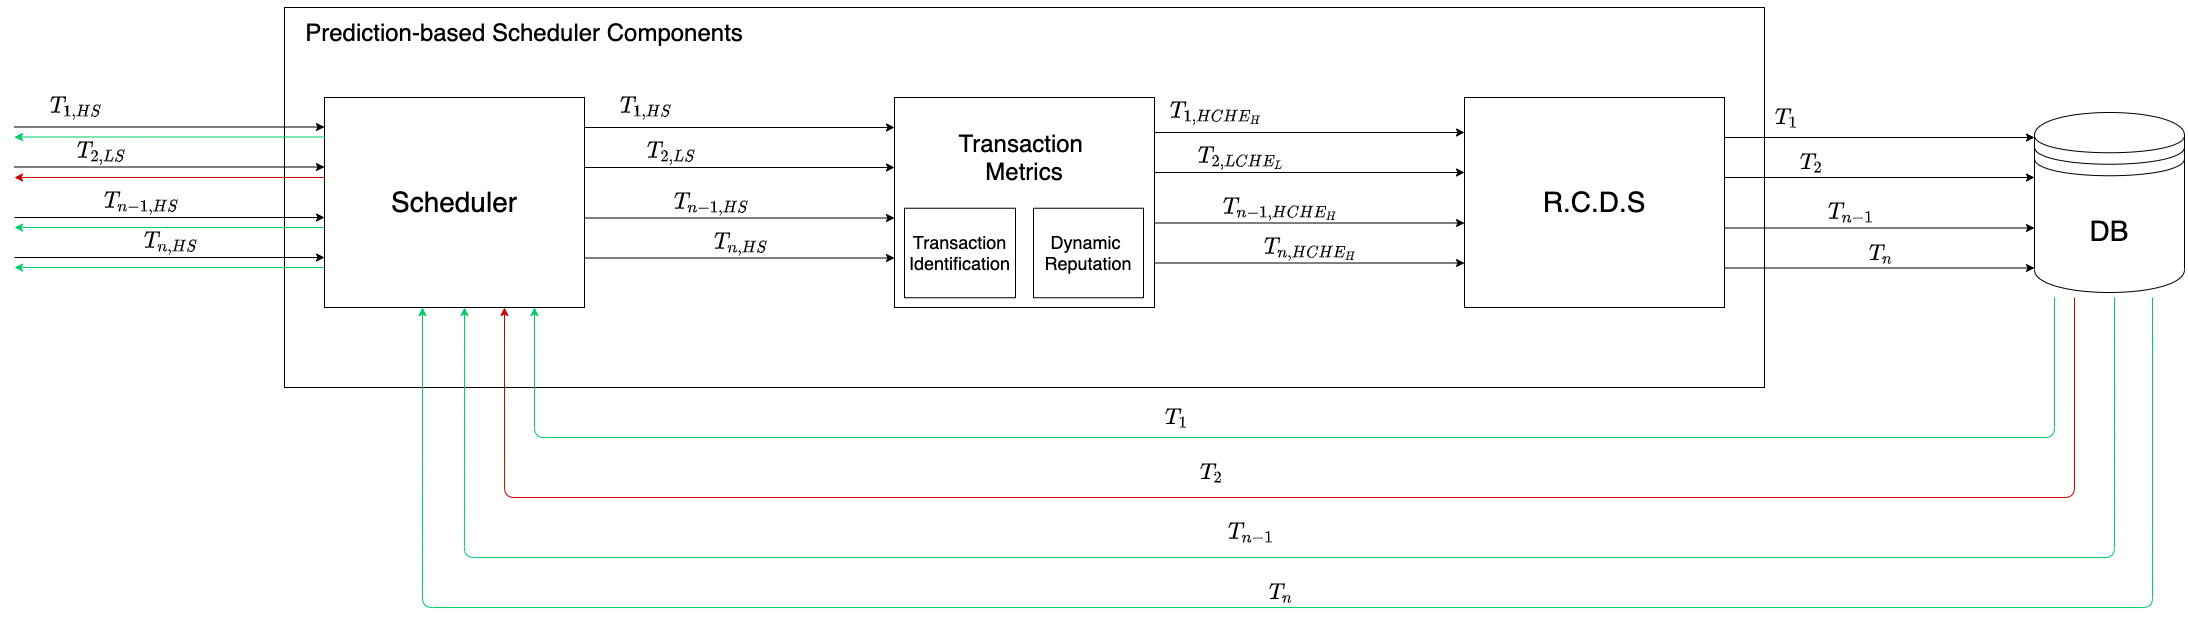
\includegraphics[width=\textwidth]{images/SystemModel_Overall}
\caption{Overall System Model of Prediction-based Scheduler}
\label{fig:system_model_overall}
\end{figure}

\subsection{Dynamic Reputation for Transactions}
In the previous section, the categorization of the transaction is assumed in order to continue forward with the decision model. This section of the dissertation involves the work needed to establish a dynamic reputation management system to allow for dynamic reputation. It involves building a reputation score for each transaction based on the transactions ranking of efficiency, commits, system aborts, and user aborts. Once a reputation score is provided we can then use dynamic reputation management to dynamically promote and demote transactions. This then allows the system to adapt to its environment dynamically. The work discussed in this area is documented in Chapter \ref{chap:dynamic_reputation}.

% Figure \ref{fig:system_model_overall} displays the system model for the work done for transactional correctness and building a dynamic reputation for transactions.
\section{Dissertation Outline}
The rest of this dissertation is organized as follows: Chapter \ref{chap:prediction_based_scheduler} outlines the research done in regards to transactional correctness while preserving concurrent operations within a web service environment. This work is published in \cite{ravan_ensuring_2020}. Chapter \ref{chap:dynamic_reputation} addresses the research done in order to build a reputation for a given transaction that is dynamic to its environment and its changing attributes. This work is submitted to ACM Transactions on Information Systems and awaiting response. Chapter \ref{chap:outline} contains the outline of the dissertation. Chapter \ref{chap:future_work} addresses the future work needed to adapt the prediction-based scheduler in Chapter \ref{chap:prediction_based_scheduler} and Chapter \ref{chap:dynamic_reputation} to a multi-level secure database and other possible solutions. Chapter \ref{chap:conclusion} contains the concluding remarks regarding all areas of research.
    %% Calls Introduction.tex
                          %% Honors theses are required to 
                          %% have an Introduction.  For
                          %% Honors theses, the file 
                          %% Introduction.tex should begin
                          %%
                          %% \chapter*{Introduction}
                          %% followed by the text of the 
                          %% introduction.
                          
\chapter{Prediction-Based Scheduler}\label{chap:prediction_based_scheduler}

\section{Overview}
\label{pbs:overview}
In this chapter, we provide the motivation and use case scenario for the work presented in this proposal. The problem defined here is the primary motivation for the current work and the anchor for the dissertation outline in Chapter \ref{chap:outline}. The work presented in Chapter \ref{chap:prediction_based_scheduler} is taken from \cite{ravan_ensuring_2020}.

\section{Introduction}
\label{pbs:introduction}
Consistency among multiple interleaved transactions in a web service context has always been an issue for researchers and database administrators. Isolation and atomicity are two of the four \ac{ACID}\footnote{The four traditional database properties are Atomicity, Consistency, Isolation, and Durability} properties that are often relaxed in order to prevent a performance bottleneck. However, when these properties are relaxed, the database can reach an inconsistent state when concurrent transactions interleave incorrectly. This causes data to become corrupted, expensive compensation transactions to be executed, and cascading rollbacks on multiple nodes to be completed before processing can continue. By looking at a practical use case we can more clearly see the issue and the need for a solution that ensures consistency. In Figures \ref{fig:e_com_ticket} \& \ref{fig:bp_env}, we see five web services executing on three different database instances. The first four web services  create a common business process created by the Business Process Execution Language (\ac{BPEL}) \cite{BPEL}. The web services are: $WS_{1}$ (decrement inventory by product ID), $WS_{2}$ (process payment), $WS_{3}$ (add order by user ID), and $WS_{4}$ (delete user payment info). The goal of the process is to allow a customer to purchase a product from an e-Commerce site. $WS_{5}$ (delete user payment info) and $WS_{3}$ execute within the same database instance. With the relaxed properties in the web service context, concurrent executions of $WS_{5}$ and $WS_{3}$ could cause an inconsistent state on $Node_{3}$. This would then cause a cascading rollback to execute and revert the committed operations of $WS_{1}$ and $WS_{2}$. Existing research shows that many solutions have been presented in the past to address this issue (e.g., \cite{Fekete_SnapshotIso}, \cite{Alrifai_Distributed_Managment}, \cite{Fekete_RAMP}, \cite{Fekete_IsolationSupport}, \cite{Jacobi_Locking}, and \cite{Fekete_Promises}). The most influential research that inspired the prediction-based solution was the Promises Model.

The Promises model presented by Alan Fekete et al. (e.g., \cite{Fekete_IsolationSupport} and \cite{Fekete_Promises}) is an elegant solution that "promises" a particular transaction that the requested resource will be available while allowing concurrent transactions to still execute on that resource. The Promises solution is robust in that it allows the "strengthening" or "weakening" of promises after they have already been made. This allows existing promises on resources to be modified without breaking the existing promise entirely. However, the solution introduces backwards compatibility issues along with a potential bottleneck at the occurrence of registering a promise for a particular transaction. 

Our prediction-based solution allows transactions to build a reputation linked to a category (categories are defined in Definition \ref{transaction_categories} \& \ref{cat_dominance}). The priorities associated with the category impact the transaction's scheduling in order to prevent cascading rollbacks. There are lock behaviors associated with the categories that enable preemptive scheduling in order to increase efficiency. The contributions in the prediction-based solution address the two issues of efficiency and consistency where existing research solutions fall short. Section \ref{pbs:problem_def} outlines the problem along with a use-case scenario. Section \ref{pbs:related_work} discusses the existing research that has already taken place in regards to the problem. Section \ref{pbs:system_model} outlines the system model for the solution. Section \ref{pbs:algorithms} discusses the algorithms needed for the solution and their psuedocode. Section \ref{pbs:analysis} provides the formal proofs for the given solution. Section \ref{pbs:experimentation} illustrates the simulation results gathered from the prototype.
\section{Problem Definition}
\label{pbs:problem_def}
Transactions in traditional database systems satisfy the four ACID  properties: Atomicity, Consistency, Isolation, and Durability. ACID transactions guarantee leaving the database in a consistent state. However, in a web service environment ACID properties and transactional concurrency cannot be fulfilled, due to performance issues. Common occurrences in web service environments involve the collaboration of multiple web services to fulfill a particular task without coupling all the needed operations in one service. Languages, such as BPEL (Business Process Execution Language) \cite{BPEL}, allow a large majority of these business processes to execute web services that must access the underlying database management systems (DBMS). These transactions may be required to relax the isolation property of the database in order to accommodate concurrent transactions.

In the event that a transaction fails (abort), and there are transactions depending on the successful execution of the failed transaction, a cascading rollback must occur, due to the inconsistency of the database. This occurs often in the web service environment due to the relaxed atomicity and isolation properties. The relaxation of the atomicity property allows operations within a transaction to commit any changes performed by the operation permanently before the entire transaction has been completed. The relaxation of the isolation property allows the interleaved execution of operations on a particular resource from concurrent transactions. This improves performance tremendously; however, in the event an operation fails, causing an abort to be issued, every transaction depending upon the failed operation must be aborted as well in order to restore consistency. These compensation transactions have become a standard practice in web service environments but sacrifice the consistency of the system. The next section will discuss a use-case scenario where this problem exists.

\subsection{Use-Case Scenario}
\label{subsec:use_case}
Assume that an e-commerce web site allows users to purchase products through an online interface. When a customer places an order a ticket is generated (see Figure \ref{fig:e_com_ticket}) containing information about the user and purchase. The ticket from the site is then handed off to a business process (starting at $WS_{1}$ in Figure \ref{fig:bp_env}) containing multiple web services, on multiple databases in a distributed context. Figure \ref{fig:bp_env} displays the architecture of the back-end business process in sequence.

\begin{figure}[h]
\captionsetup{justification=centering}
\centering % used for centering Figure

\begin{tikzpicture}
  \draw (0,0) -- (0,2.02) -- (1.6,2.02) -- (1.6,1.7) -- (1.9,1.7) -- (1.9,0) -- cycle;
  \draw (1.6,2.02) -- (1.9,1.7);
  \node[text width=1.5cm] at (.85,1.25) {$userID$};
  \node[text width=1.5cm] at (.85,.75) {$productID$};
  \node[text width=1.5cm] at (.85,.3) {$cardID$};
  \draw[thick,->] (2.25,1.25) -- (2.85,1.25);
  \draw[thick,->] (2.25,.75) -- (2.85,.75);
  \draw[thick,->] (2.25,.3) -- (2.85,.3);
  \node[text width=6cm] at (6,1.25) {"jravan"};
  \node[text width=6cm] at (6,.75) {"20lb-coffee"};
  \node[text width=6cm] at (6,.3) {"5258-9663-4625-1489"};
\end{tikzpicture}

\caption{e-Commerce Web Site Ticket Example} % title of the Figure
\label{fig:e_com_ticket} %% label to refer figure in text

\end{figure}

\begin{figure}[h]
\captionsetup{justification=centering}
\centering % used for centering Figure

\begin{tikzpicture}
    \node [webservice, anchor=north] (ws4) {$WS_{4}$};
    \node [webservice, above=2cm of ws4.north, anchor=north] (ws3) {$WS_{3}$};
    \node [webservice, above=2cm of ws3.north, anchor=north] (ws2) {$WS_{2}$};
    \node [webservice, above=2cm of ws2.north, anchor=north] (ws1) {$WS_{1}$};
    \node [draw, cylinder, shape border rotate=90, aspect=0.75, %
      minimum height=30, minimum width=30, anchor=north, left=.5cm of ws3] (data3) {DB};
    \node [draw, cylinder, shape border rotate=90, aspect=0.75, %
      minimum height=30, minimum width=30, above=2cm of data3.north, anchor=north] (data2) {DB};
    \node [draw, cylinder, shape border rotate=90, aspect=0.75, %
      minimum height=30, minimum width=30, above=2cm of data2.north, anchor=north] (data1) {DB};
    \node [webservice, left=4cm of ws3.north, anchor=north] (ws5) {$WS_{5}$};
    \path [line] (ws1) -- (data1);
    \path [line] (ws2) -- (data2);
    \path [line] (ws3) -- (data3);
    \path [line] (ws1) -- (ws2);
    \path [line] (ws2) -- (ws3);
    \path [line] (ws3) -- (ws4);
    \path [line] (ws5) -- (data3);
    \draw[dotted,blue] (-5.25,.35) rectangle (3,-1.55);
    \draw[dotted,red] (-5.25,2.35) rectangle (3,.45);
    \draw[dotted,black] (-5.25,4.35) rectangle (3,2.45);
    \draw[dotted,purple] (-5.25,6.35) rectangle (3,4.45);
    \node[text width=1cm] at (2,6) {$Node_{1}$};
    \node[text width=1cm] at (2,4) {$Node_{2}$};
    \node[text width=1cm] at (2,2) {$Node_{3}$};
    \node[text width=1cm] at (2,0) {$Node_{4}$};
    \node[text width=9cm] at (-.5,-2) {$WS_{1} = Decrement Inventory By Product ID$};
    \node[text width=7cm] at (-.5,-2.5) {$WS_{2} = Process Payment$};
    \node[text width=7cm] at (-.5,-3) {$WS_{3} = Get Order By User ID$};
    \node[text width=7cm] at (-.5,-3.5) {$WS_{4} = Generate Receipt$};
    \node[text width=7cm] at (-.5,-4) {$WS_{5} = Delete Order By User ID$};
\end{tikzpicture}

\caption{Business Process for e-Commerce Web Site} % title of the Figure
\label{fig:bp_env} % label to refer figure in text

\end{figure}

Each dotted rectangle within Figure \ref{fig:bp_env} represents a distributed node containing a public web service executing transactions on an underlying database. In order for a successful purchase to take place within the e-commerce environment, the business process containing the web service sequence $WS_{1}, WS_{2}, WS_{3},$ and $WS_{4}$ must execute successfully. $WS_{1}$ ($DecrementInventoryByProductID$) uses the $productID$ provided from the current ticket in order to query the database regarding the requested product. $WS_{2}$ ($ProcessPayment$) uses the payment information provided in the ticket to charge the user. $WS_{3}$ ($GetOrderByUserID$) is a service that takes the given $userID$ and $product ID$, and returns a record of purchase for the user. $WS_{4}$ ($GenerateReceipt$) simply generates a receipt from the ticket information and is returned to the user's interface. Once $WS_{4}$ has completed processing, and only when it is finished, a purchase is considered successful.

The issue is that multiple web services may be executed on a single database instance. Without concurrency control, interleaved executions, such as the case with $WS_{3},$ and $WS_{5}$, may cause inconsistencies. 

% \subsection{Use Case Transactions for $Node_{3}$}
% \label{sec:use_case_for_node_3}
% In Figure \ref{fig:webform}, we see the contents of the two transactions executing on $Node_{3}$. $T_{DeleteOrderByUserID}$ is a transaction generated by $W_{5}$. The responsibility of this web service is to determine if the user exists, and if they do exist, to delete the user's order information from the database by the provided \textit{userID}. The transaction generated by $WS_{3}$ ($T_{GetOrderByUserID}$, mentioned above from Figure \ref{fig:bp_env}) is responsible for getting an order from a user account. This transaction executes under the pretext that the \textit{userID} given exists in the database or the web service would not have been able to be executed. If $T_{GetOrderByUserID}$ fails within the business process outlined in Figure \ref{fig:bp_env}, then an abort must be issued, and all the previous operations committed from $WS_{1}$ and $WS_{2}$ must be rolled back. This includes operations that were executed from subsequent transactions that depended on the results of $WS_{1}$ and $WS_{2}$.

Assume $WS_{3}$ and $WS_{5}$ are $T_{GetOrderByUserID}$ and $T_{DeleteOrderByUserID}$. The deletion transaction contains four operations: $R_{2}(b)$, $W_{2}(b)$, $R_{2}(a)$, and $W_{2}(a)$. The transaction will first READ from the database to ensure the user exists and then WRITE out the order information if the order does exist\footnote{In this instance the WRITE operation executed would write a $NULL$ or empty record to the database in order to "delete" the record.}. The other transaction, $T_{GetOrderByUserID}$, contains a single $R_{1}(a)$ and $R_{1}(b)$. Each transaction contains a $C_{i}$ operation that represents the COMMIT operation that the database executes after all operations have completed. Figure \ref{fig:webform} shows the two transactions along with the operations contained within.

\begin{figure}[h]
\captionsetup{justification=centering}
\centering % used for centering Figure

\begin{picture}(50,40)
    \put(-80.5,25){$W_{3} = T_{GetOrderByUserID}$ = $R_{1}(a)R_{1}(b)C_{1}$}
    \put(-97,10){$W_{5} = T_{DeleteOrderByUserID}$ = $R_{2}(b)W_{2}(b)R_{2}(a)W_{2}(a)C_{2}$}
\end{picture}

\caption{e-Commerce Web Service Transaction Sequences} % title of the Figure
\label{fig:webform} % label to refer figure in text

\end{figure}

% \subsection{Use Case Transaction Metrics}
For the transactions listed above, we know the commit rate, number of transactions executed, and the average execution time. Commit rate is the percentage of successful commits over the total amount of attempted executions of that particular transaction (Definition \ref{cmt_rate}). Number of transactions represents the total number of executions attempted (commits and aborts combined) for that particular transaction. Efficiency rate represents the average efficiency of the particular transaction to reach a completion state; whether it is a failure or success (Definition \ref{eff_rate}). A transaction with a very long execution time will have an efficiency rate that is much lower than a transaction that executes and completes very quickly. The attribute data listed previously is consolidated into Table \ref{tbl:trans_metrics} below. 
\\
\begin{table}[h]
\captionsetup{justification=centering}
\centering
\begin{tabular}{|c|c|c|c|c|}
\hline
\multicolumn{4}{|c|}{\cellcolor[HTML]{EFEFEF}\textbf{Transaction Metrics}}                                                   \\ \hline
\textbf{Transactions} & \textbf{Commit Rate} & \textbf{\# of Trans.} & {\color[HTML]{000000} \textbf{Eff. Rate}} \\ \hline
$T_{DeleteOrderByUserID}$         & 98\%                  & 200                         & 98\%                                          \\ \hline
$T_{GetOrderByUserID}$          & 97\%                     & 520                           & 99\%                                              \\ \hline
\end{tabular}

\caption{Transaction Metrics} % title of the Figure
\label{tbl:trans_metrics} % label to refer figure in text

\end{table}

In a web service context, without the prediction-based solution, the isolation property will be relaxed and a serializable execution will be created. This serializable execution will be based on the conflicting operations of the two transactions. Figure \ref{fig:combined_history} displays an example of a generated serializable execution from $T_{GetOrderByUserID}$ and $T_{DeleteOrderByUserID}$.

\begin{figure}[h]
\captionsetup{justification=centering}
\centering % used for centering Figure

\begin{picture}(50,25)
    \put(-90,5){$T_{Schedule}$ = $R_{1}(a)R_{2}(b)R_{1}(b)W_{2}(b)R_{2}(a)W_{2}(a)$}
\end{picture}

\caption{Generated Schedule} % title of the Figure
\label{fig:combined_history} % label to refer figure in text

\end{figure}

The schedule listed in Figure \ref{fig:combined_history} is a well-formed serializable schedule. Between each operation within the schedule, a commit operation $C_{i}$ is executed. This shows how the Atomcity property of a database is relaxed during the execution of a schedule. Therefore, if $R_{2}(a)$ fails, a cascading rollback will be issued causing the operations of $T_{GetOrderByUserID}$ to be rolled back regardless of their successful execution. The operations of $T_{GetOrderByUserID}$ must be rolled back since they are a part of $T_{Schedule}$ and a COMMIT operation has been executed already. If $T_{GetOrderByUserID}$ was executed as a part of the business process outlined in the use case, then the operations of the previous web services ($WS_{1}$ and $WS_{2}$) must be rolled back.

Conversely, if the data in Table \ref{tbl:trans_metrics} were taken into consideration before generating the serializable execution, $T_{GetOrderByUserID}$ could be given a more restrictive concurrency control mechanism, such as locking. Table \ref{tbl:trans_metrics} contains data that proves instances of $T_{GetOrderByUserID}$ have a high rate of commit with a high percentage of efficiency throughout the system. Table \ref{tbl:trans_metrics} also displays that instances of $T_{DeleteOrderByUserID}$ could use locking techniques due to its history. Therefore, $T_{GetOrderByUserID}$ and $T_{DeleteOrderByUserID}$ could execute within the same schedule using traditional locking techniques, commit changes quickly and successfully, and prevent a cascading rollback from reverting the effects of $WS_{1}$ and $WS_{2}$ by using the reputation provided by the separate transactions. In the proposed solution, we aim to provide concurrency control that is based on the metadata of the transactions. Our hypothesis is that if transactions could be treated differently based on their history, stronger concurrency control techniques could be leveraged, such as locking, which ensures the consistency property for web service transactions. Section \ref{pbs:analysis} walks through this exact use-case scenario with two-phase locking and the proposed prediction-based solution. The next section will discuss the existing research that has taken place to remediate this problem without the current knowledge of transaction metrics.
\section{Related Work}
\label{pbs:related_work}

Ensuring successful concurrency control in web service transactions has been studied in depth for some time (e.g., \cite{Fekete_Promises}, \cite{Fekete_IsolationSupport}, \cite{Alrifai_Distributed_Managment}, \cite{dai_qos-driven_2009}, \cite{zhengdong_gao_combining_2005}, \cite{ferreira_transactional_2012}, \cite{kang-woo_lee_consistency_2000}, and \cite{olmsted_long_2015}). The Promises model presented by Alan Fekete et al. (e.g., \cite{Fekete_Promises} and \cite{Fekete_IsolationSupport}) is an elegant solution that "promises" a particular transaction that the requested resource will be available while allowing concurrent transactions to still execute on that resource. Alomari et al. present a solution involving an External Lock Manager (\gls{elm}) that resides outside of the \gls{dbms} \cite{Fekete_SnapshotIso}. This allows a layer of separation between the application and the \gls{dbms} in order to schedule transactions using special business logic according to the environment. In the solution presented by Alrifai et al. \cite{Alrifai_Distributed_Managment}, an edge chasing solution using dependency graphs is incorporated in order to detect dependencies between globally scheduled transactions. The solution was tested parallel to the well known 2-Phase Locking Protocol (\gls{2pl}) and provided promising results regarding efficiency. However, the Alrifai et al. solution becomes less efficient when the number of dependency cycles are detected. The model of the different lock types comes from Christian Jacobi et al. \cite{Jacobi_Locking} with research in concurrent locking with parallel database systems. The researchers extended the use of the native lock types in the existing database structure in order to speed up thread processing on multi-processor machines. Prediction-based concurrency control has been proposed by Eunhee Lee et al. \cite{Eunhee_PredictionBasedCC} with the entity-radius solution. This solution uses the concept of multiple entity radii that attempts to predict the next user based on their location. The prediction is generated from the location within a radius of the replicated site and their navigation speed. The solution provided is elegant with excellent experimental results but no formal proof or analysis of the algorithm is provided. Other solutions to prevent business process cancellation or rollback when participants of the process do not behave correctly involve global views of the process \cite{Fekete_RAMP}, \cite{Riegen_RuleBased}. Support for these types of solutions are based on the well-known Oasis specifications of WS-Coordination, WS-AtomicTransaction, and WS-BusinessActivity \cite{WSCO}, \cite{WSAT}, \cite{WSBA}. These solutions are well-designed; however, they require the presence of a global coordinator throughout the entire business process. In the next section, we will discuss the prediction-based solution's system model generated from the current available work in the research community.

%%%%%% BEGINNING OF SYSTEM MODEL SECTION %%%%%%%
\section{System Model}
\label{pbs:system_model}
This section outlines the system model on which the solution is built. Definitions for new concepts are introduced first, considering they will be used to describe the different components that consist of the system model. Later subsections explain in detail the different components and processes required for the prediction-based solution. We assume that all the transactions are well-formed and the scheduler is legal.

\subsection{Definitions}
\label{pbs:definitions}

\defCommitRate{cmt_rate}
\defEfficiencyRate{eff_rate}

\begin{definition}
\label{cat_bounds}
 (Categorization Thresholds) - categorization thresholds are upper and lower limits of both commit rate and efficiency rate that are used when categorizing transactions\footnote{The categorization bounds are static values that do not change throughout the system execution. Both the efficiency rate and the commit rate bounds are currently at 50\% creating full coverage of all transactions.}.
\end{definition}

% \begin{definition}
% \label{cat_threshold}
%  (Categorization Thresholds) - categorization thresholds are calculated within the categorization bounds (see Definition \ref{cat_bounds}) by using the Transaction Concentration Ratio (see Section \ref{sec:TCR}). The threshold values are dynamic and change depending on the execution environment but will not exceed the categorization bounds placed on that particular category. Categorization thresholds enforce the most accurate thresholds for the execution environment while allowing flexibility.
% \end{definition}

\begin{definition}
\label{transaction_categories}
(Transaction Categories) - Let $T$ = \{$T_{1}$, ... , $T_{n}$\} be a set of transactions and $C$ = \{$HCHE$, $HCLE$, $LCHE$, $LCLE$\} a set of category names. The mapping $\tau$ associates a category name with each transaction as follows:

\[ 
\tau : \textrm{$T_{i}$}\rightarrow
\left \{
  \begin{tabular}{cc}
  HCHE & if $C_{r}(T_{i}) > 0.5$ and $E_{r}(T_{i}) > 1$ \\
  HCLE & if $C_{r}(T_{i}) > 0.5$ and $E_{r}(T_{i}) \le 0.5$ \\
  LCHE & if $C_{r}(T_{i}) \le 0.5$ and $E_{r}(T_{i}) > 1$ \\
  LCLE & if $C_{r}(T_{i}) \le 0.5$ and $E_{r}(T_{i}) \le 0.5$
  \end{tabular}
\right \}
\]

{\normalfont In order to ensure correct lock techniques are selected, transactions cannot be simply characterized as good or bad based on their metrics. For example, a transaction $T_{1}$ may have a 100\% commit rate, but it may have a long execution time. A transaction with these characteristics should not be penalized when, in fact, it is a well behaving transaction. On the other hand, a transaction $T_{2}$ that has a 100\% commit rate and has an extremely short execution time should not be treated with the same priority as $T_{1}$. This is where certain of levels must be established to ensure the most appropriate selection is made.

In order to establish levels, a system of categories was put in place base on the metrics mentioned previously. The first categorization is based solely on the efficiency of the transaction. In this categorization, there are two attributes: \textit{high efficiency (HE)} and \textit{low efficiency (LE)}. A transaction that has been labeled as \textit{HE} is considered to execute with an efficiency in the upper 50\% of all transactions executed within the system\footnote{See Section \ref{pbs:cat_graph} and Section \ref{pbs:definitions} for more clarification}. The second attribute, \textit{LE}, is any transaction where its efficiency rate is in the lower 50\% of all transactions executed.

The second categorization that the levels are built on is based solely on the outcome of the transaction. These attributes are \textit{high commit (HC)} and \textit{low commit (LC)}, which are much more simple to define. A transaction with a \textit{HC} attribute has committed successfully over 50\% of executions (upper 50\% of all transactions). A transaction with an \textit{LC} attribute has failed over 50\% of its executions (lower 50\% of all transactions). This categorization correlates directly with the commit rate defined (see Definition \ref{cmt_rate}).

With these two categorizations and two attributes, a four-level system was devised in order to select appropriate lock types. The four categories devised are \textit{high commit-high efficiency (HCHE)}, \textit{high commit-low efficiency (HCLE)}, \textit{low commit-high efficiency (LCHE)}, and \textit{low commit-low efficiency (LCLE)}. Depending on the level in which the transaction has been placed, different lock types will be granted in order to perform concurrency control.}

\end{definition}

\begin{definition}
\label{cat_dominance}
(Transaction Category Dominance) - The Transaction Category Dominance is a pair, denoted as $C_{D} = (C,L)$, where $C$ is the set of transaction categories, and $L$ is a partial order of the categories such that:
 
\[\textrm{$HCHE > HCLE > LCLE$}\]
\[\textrm{$HCHE > LCHE > LCLE$} \]

\begin{figure}[h]
\captionsetup{justification=centering}
\centering % used for centering Figure

\begin{tikzpicture}
    % [list/.style={rectangle split, rectangle split parts=3,
    % draw, rectangle split horizontal}, >=stealth, start chain]
  \node[text width=1.5cm] at (3.8,5) {$HCHE$};
  \node[text width=1.5cm] at (2.8,4) {$HCLE$};
  \node[text width=1.5cm] at (4.8,4) {$LCHE$};
  \node[text width=1.5cm] at (3.8,3) {$LCLE$};
  \draw (3.55,4.8) -- (2.7,4.2);
  \draw (3.75,4.8) -- (4.7,4.2);
  \draw (3.55,3.2) -- (2.7,3.8);
  \draw (3.75,3.2) -- (4.7,3.8);
  
\end{tikzpicture}

% \caption{Web Service Environment with Scheduler} % title of the Figure
\label{fig:category_lattice} % label to refer figure in text

\end{figure}

{\normalfont Note that the categories $HCLE$ and $LCHE$ are not comparable. That is, we cannot establish a dominance relation between transactions in $HCLE$ and $LCHE$ categories.

However, in our model, we focus on reducing the need of compensation for aborted transactions. Therefore, we prioritize the commit property over the efficiency property. We introduce the dominance relation below in Table \ref{tbl:priority}.}

\[\textrm{$HCLE > LCHE$} \]
 
\begin{table}[h]
\captionsetup{justification=centering}
\centering
\begin{tabular}{l|c|}
\cline{2-2}
                                          & \multicolumn{1}{l|}{\textbf{Priority}} \\ \hline
\multicolumn{1}{|l|}{\textbf{HCHE}}  & I                                      \\ \hline
\multicolumn{1}{|l|}{\textbf{HCLE}}  & II                                     \\ \hline
\multicolumn{1}{|l|}{\textbf{LCHE}} & III                                     \\ \hline
\multicolumn{1}{|l|}{\textbf{LCLE}} & IV                                      \\ \hline
\end{tabular}

\caption{Category Priorities} % title of the Figure
\label{tbl:priority} % label to refer figure in text

\end{table} 

\end{definition}

% \begin{definition}
% \label{min_commit}
% (HCHE) - HCHE, acronym for High Commit High Efficiency, is a transaction categorization with categorization bounds (see Definition \ref{cat_bounds}) that involve a commit rate of 50\% and higher and a efficiency rate in the upper 50\% and higher as well (see Definitions \ref{cmt_rate} and \ref{eff_rate}). Table \ref{tbl:default_tmetrics} outlines all transaction categories.
% \end{definition}

% \begin{definition}
% \label{min_abrt}
% (LCHE) - LCHE, acronym for Low Commit High Efficiency, is a transaction categorization with categorization bounds (see Definition \ref{cat_bounds}) that involve a commit rate of 50\% and lower and a efficiency rate in the upper 50\% and higher (see Definitions \ref{cmt_rate} and \ref{eff_rate}). Table \ref{tbl:default_tmetrics} outlines all transaction categories.
% \end{definition}

% \begin{definition}
% \label{ext_commit}
% (HCLE) - HCLE, acronym for High Commit Low Efficiency, is a transaction categorization with categorization bounds (see Definition \ref{cat_bounds}) that involve a commit rate of 50\% and higher and a efficiency rate in the bottom 50\% and lower (see Definitions \ref{cmt_rate} and \ref{eff_rate}). Table \ref{tbl:default_tmetrics} outlines all transaction categories.
% \end{definition}

% \begin{definition}
% \label{ext_abrt}
% (LCLE) - LCLE, acronym for Low Commit Low Efficiency, is a transaction categorization with categorization bounds (see Definition \ref{cat_bounds}) that involve a commit rate of 50\% and lower and a efficiency rate in the bottom 50\% and lower as well (see Definitions \ref{cmt_rate} and \ref{eff_rate}). Table \ref{tbl:default_tmetrics} outlines all transaction categories.
% \end{definition}

%\begin{definition}
%\label{no_trend}
%(NO\_TREND) - NO\_TREND is a transaction categorization with categorization bounds (see Definition \ref{cat_bounds}) that include all %the outlining space that the previous four categories do not include. If the efficiency rate is less than or equal to 25\% then the %commit rate must be between 25\% and 75\% (see Definitions \ref{cmt_rate} and \ref{eff_rate}). If the efficiency rate is between 25\% %and 75\% then the commit rate includes all values ranging from 0\% to 100\%. Finally, if the efficiency rate is greater than or equal %to 75\% then the commit rate must be between 25\% and 75\%. Table \ref{tbl:default_tmetrics} outlines all transaction categories.
%\end{definition}

%\[
%\left \{
%  \begin{tabular}{ll}
%  
%  $E_{r}\le25\%$, & $25\%<C_{r}<75\%$ \\
%  $25\%<E_{r}<75\%$, & $0\%\le C_{r}\le100\%$ \\
%  $E_{r}\ge75\%$, & $25\%<C_{r}<75\%$
%  
%  \end{tabular}
%\right \}
%\]

\begin{definition}
\label{conflict_ops}
 (Conflicting Operations) - two operations are conflicting:

 \begin{enumerate}
   \item they are contained within two different transactions,
   \item both operations are operating on the same data item, and
   \item at least one of the operations is a WRITE
 \end{enumerate}

 \begin{example}
 \label{ex_conflict_ops}
  Let $o_{1}$ be a READ operation on data item $User ID$ in transaction $T_{1}$ and let $o_{2}$ be a WRITE operation on $User ID$ in $T_{2}$. These two operations are conflicting.
 \end{example}
\end{definition}

% \begin{definition}
% \label{conflict_trans}
%  (Conflicting Transactions) - two transactions are considered conflicting if they contain all of the following attributes:
 
%  \begin{enumerate}
%  \item both transactions contain conflicting operations (see Definition \ref{conflict_ops})
%  \item both transactions are contained within the same serializable schedule
%  \item and at least one of the transactions is categorized to abort
%  \end{enumerate}
 
%  \begin{example}
%  \label{ex_conflict_trans}
%   Using the transactions mentioned in Example \ref{ex_conflict_ops} let's say the serializable schedule $S_{1}$ contains   an interleaved execution of $T_{1}$ and $T_{2}$. These transactions are now considered conflicting.
%  \end{example}
% \end{definition}

% \begin{definition}
% \label{conflict_cat}
%   (Conflicting Categories) - conflicting categories are very much related to conflicting transactions (see Definition \ref{conflict_trans}) however this definition is concerned with the categories the transactions have been placed in rather than the transactions themselves. Two categories are said to be conflicting if they contain all of the following attributes:
  
%   \begin{enumerate}
%   \item both are contained within the same serializable schedule
%   \item and at least one of the categories is predicted to abort
%   \end{enumerate}
  
% Transactions of conflicting categories are not allowed within the same schedule within this solution.  
  
%   \begin{example}
%   For example, let's say we have transaction $T_{1}$ that has been placed in the category HCHE and transaction $T_{2}$ that has been placed in the category LCLE. These two categories are considered conflicting even if $T_{1}$ and $T_{2}$ are not considered to be conflicting transactions themselves.
%   \end{example}
  
% \end{definition}

% \begin{definition}
% \label{serial_sched}
%  (Serializable Schedule) - a serializable schedule is a non-serial schedule that can be converted to a serial schedule by interchanging non-conflicting operations (see Definition \ref{conflict_ops})

% \end{definition}

% \begin{definition}
% \label{casc_rollback}
%  (Cascading Rollback) - a cascading rollback occurs when two conflicting transactions (see Definition                     \ref{conflict_trans}) are interleaved within the same serializable schedule. The abort is cascading in the sense that an  abort must be issued for each transaction within the schedule that was dependant upon the transaction that issued the abort. This is needed to ensure a consistent state within the database.
 
%  \begin{example}
%  \label{ex_casc_rollback}
%   Using the serializable schedule generated in Example \ref{ex_conflict_trans}, if transaction $T_{2}$ issues an abort then  transaction $T_{1}$ must also be aborted since $T_{1}$ is dependant upon $T_{2}$.
%  \end{example}
 
% \end{definition}

\begin{definition}
\label{compatibility}
(Compatibility) - a data item is locked in a non-compatible mode if:

\begin{enumerate}
  \item the data item is locked by write-lock, or
  \item the data item requesting the lock is categorized with a lower priority
\end{enumerate}
\end{definition}

\begin{definition}
\label{legal_scheduler}
 (Legal Scheduler) - a prediction-based scheduler is legal if:
 
 \begin{enumerate}
    \item \textbf{Grant:} (denoted as the addition symbol, +) a transaction is permitted to lock a data item if the data item is not already locked in a non-compatible mode (see Definition \ref{compatibility}) by an other transaction\footnote{In the event that a lock is requested of a resource that has not issued any locks, then the lock will be automatically granted. There is no conflict, and therefore, the compatibility matrices do not apply.}.
    \item \textbf{Decline:} (denoted as the subtraction symbol, -) a transaction $T_{i}$ is denied to lock a data item if the data item is already locked in a non-compatible mode (see Definition \ref{compatibility}) by another transaction $T_{j}$ where $\tau(T_{i}) \le \tau(T_{j})$
    \item \textbf{Elevate:} (denoted as lowercase delta, $\delta$) a transaction $T_{i}$ is permitted to lock a data item if all the non-compatible locks (see Definition \ref{compatibility}) on the data item are being held by transactions $T_{1}, ... , T_{k}$ such that $\tau(T_{j}) < \tau(T_{i})$ for all $j = 1, ..., k$ in this case $T_{1}, ... , T_{k}$ must first release the locks on the data item before $T_{i}$ is permitted to lock the data item.
 \end{enumerate}

% \begin{definition}
% \label{grant_action}
%  (Grant Action) - the grant action is one of the three possible actions that can take place within the two lock compatibility matrices (Table \ref{tbl:read_lock_compatibility} \& Table \ref{tbl:write_lock_compatibility}). This action is represented by the plus sign (+) which signifies that there is not a conflict between the granted and requesting transactions and the lock can be granted to the transaction that is requesting access to the resource.
 
 \begin{example}
 \label{ex_grant_action}
  A read-lock for a data item $R$ has been granted to transaction $T_{1}$ within the $HCHE$ transactional category. Transaction $T_{2}$ within the $HCLE$ is also requesting a read-lock on data item $R$. This does not cause a conflict and therefore the grant action will be taken and the requested lock will be issued to $T_{2}$.
 \end{example}
 
% \end{definition}

% \begin{definition}
% \label{decline_action}
%  (Decline Action) - the decline action is one of the three possible actions that can take place within the two lock compatibility matrices (Table \ref{tbl:read_lock_compatibility} \& Table \ref{tbl:write_lock_compatibility}). This action is represented by the minus sign (-) which signifies that there is a conflict between the granted and requesting transactions and the lock can not be granted to the transaction that is requesting access to the resource.
 
 \begin{example}
 \label{ex_decline_action}
  A write-lock for a data item $R$ has been granted to transaction $T_{1}$ within the $HCHE$ transactional category. Transaction $T_{2}$ within the $HCLE$ is requesting a write-lock to data item $R$. This causes a conflict and therefore the decline action will be taken and the requested lock will not be issued to $T_{2}$.
 \end{example}
 
% \end{definition}

% \begin{definition}
% \label{elevate_action}
%  (Elevate Action) - the elevate action is one of the three possible actions that can take place within the two lock compatibility matrices (Table \ref{tbl:read_lock_compatibility} \& Table \ref{tbl:write_lock_compatibility}). This action is represented by the delta symbol ($\delta$) which signifies that the transaction requesting access to the resource is in a category that contains a higher prioritization (see Table \ref{tbl:priority}) than the transactions that currently hold locks to the resource. In this situation all locks held by transactions of lower priority will be preemptively dropped so the transaction with the higher priority can obtain the needed lock.
 
 \begin{example}
 \label{ex_elevate_action}
  A read-lock for a data item $R$ has been granted to transaction $T_{1}$ within the $LCLE$ transactional category. Transaction $T_{2}$ within the $HCHE$ is requesting a write-lock to data item $R$. However, this causes a conflict; since $T_{2}$ contains a higher priority than $T_{1}$; the elevate action will be taken and the requested lock will be issued to $T_{2}$.
 \end{example}
 
\end{definition}
\subsection{Environment}
\label{pbs:environment}
In a web services environment, multiple web services can submit transactions to a database to be executed. As mentioned before, if only one transaction can be executed at any given time, then other concurrent transactions from other web services must wait. This causes a significant performance degradation; therefore, concurrent transactions from multiple web services must be handled. This is where the Database Management System's (\ac{DBMS}) scheduler plays an important role in ensuring concurrent transactions preserve consistency within the database. The scheduler receives transactions that are submitted from web services and generates a serializable schedule based on the conflicting operations contained within the transactions. 

After receiving the concurrent transactions (e.g., $T_{1}$, $T_{2}$, ... , $T_{N}$) the scheduler is responsible for analyzing the conflicting operations within the transactions and generating a serializable schedule that will then be executed on the database itself (e.g., $T_{Sched}$). This serializable execution is guaranteed to leave the database in a consistent state after a successful execution due to the analysis performed by the scheduler and the ordering of the operations within the transaction. Figure \ref{fig:Tsched} displays the generation of $T_{Sched}$ from multiple web service transactions. Figure \ref{fig:ws_env} displays a diagram of the database scheduler in a web service context.

\begin{figure}[h]
\captionsetup{justification=centering}
\centering % used for centering Figure

\begin{picture}(55,100)
    \put(-93,80){$T_{1}$ = \{ $W_{1}(r_{1})R_{1}(r_{1})W_{1}(r_{2})R_{1}(r_{2})$ ... $W_{1}(r_{n})R_{1}(r_{n})C_{1}$ \}}
    \put(-93,65){$T_{2}$ = \{ $W_{2}(r_{1})R_{2}(r_{1})W_{2}(r_{2})R_{2}(r_{2})$ ... $W_{2}(r_{n})R_{2}(r_{n})C_{2}$ \}}
    \put(-58,50){.}
    \put(-58,45){.}
    \put(-58,40){.}
    \put(-100,23){$T_{N}$ = \{ $W_{n}(r_{1})R_{n}(r_{1})W_{n}(r_{2})R_{n}(r_{2})$ ... $W_{n}(r_{n})R_{n}(r_{n})C_{N}$ \}}
    \put(-165,18){\makebox[\linewidth]{\rule{10.65cm}{0.4pt}}}
    \put(-90,5){$T_{Sched}$ = \{ $T_{1}T_{2}$ ... $T_{N}$ \}}
\end{picture}

\caption{Generation of $T_{Sched}$ from Concurrent Web Service Transactions} % title of the Figure
\label{fig:Tsched} % label to refer figure in text

\end{figure}

\begin{figure}[h]
\captionsetup{justification=centering}
\centering % used for centering Figure

\begin{tikzpicture}
    \node [draw, cylinder, shape border rotate=90, aspect=0.75, %
      minimum height=30, minimum width=50] (data) {DB};
    \node [block, above=2cm of data.south,anchor=south] (sched) {Scheduler};
    \node [webservice, above=2cm of sched] (ws1) {$WS_{1}$};
    \node [webservice, right=of ws1] (ws2) {$WS_{2}$};
    \node [webservice, right=of ws2] (wsN) {$WS_{N}$};
    \path [line] (sched) -- (data);
    \path [line] (data) -- (sched);
    \path [line] (ws1) -- (sched);
    \path [line] (ws2) -- (sched);
    \path [line] (wsN) -- (sched);
    \put(5,105){$T_{1}$}
    \put(50,105){$T_{2}$}
    \put(95,105){$T_{N}$}
    \put(5,30){$T_{Sched}$}
\end{tikzpicture}

\caption{Web Service Environment with Scheduler} % title of the Figure
\label{fig:ws_env} % label to refer figure in text

\end{figure}

The architecture shown in Figure \ref{fig:ws_env} is a typical web service environment that currently exists. The existing web service environment treats all transactions equally. Every transaction submitted to the \ac{DBMS} scheduler is compiled into a schedule and submitted to the database. The drawback of this type of architecture is the case of a cascading rollback. In the event of a cascading rollback, operations that have successfully completed must be reverted, due to the failure of a dependant operation in a separate transaction. The prediction-based architecture used in the presented solution adds a new logical component (transaction metrics). This component is added at the scheduling level to analyze certain metadata about transactions submitted to the scheduler. Table \ref{tbl:trans_metrics} displays the type of data that will be calculated in order to make an accurate prediction on the likelihood that a transaction will either commit or abort. Once implemented, transactions will build a history, or a reputation, based on commit rate and efficiency rate. Figure \ref{fig:ws_env_with_metrics} displays the addition to the existing architecture in the prediction-based solution.
\subsection{Transaction Metrics}
\label{pbs:transaction_metrics}
The transaction metrics logical unit will contain all processing logic to accurately categorize the transactions submitted to the database. When a transaction is submitted to the scheduler to be added to a serializable schedule, the scheduler will look to the transaction metrics to determine the locking action that should be used for that particular transaction. All transaction metrics will be computed within the component before the scheduler issues a query so that the maximum time required for a response will be of complexity \textit{O(1)}. These metrics are updated as the execution environment matures and the Transaction Categorization Graph (see Section \ref{pbs:cat_graph}) becomes more densely populated. 

\begin{figure}[ht]  
\captionsetup{justification=centering}
\centering % used for centering Figure

\begin{tikzpicture}
    \node [draw, cylinder, shape border rotate=90, aspect=0.75, %
      minimum height=30, minimum width=50] (data) {DB};
    \node [block, above=2cm of data.south,anchor=south] (sched) {Scheduler};
    \node [block, right=3cm of sched.south,anchor=south, minimum width=70] (trans_met) {Transaction Metrics};
    \node [webservice, above=2cm of sched] (ws1) {$WS_{1}$};
    \node [webservice, right=of ws1] (ws2) {$WS_{2}$};
    \node [webservice, right=of ws2] (wsN) {$WS_{N}$};
    \path [line] (sched) -- (data);
    \path [line] (data) -- (sched);
    \path [line] (ws1) -- (sched);
    \path [line] (ws2) -- (sched);
    \path [line] (wsN) -- (sched);
    \path [line] (trans_met) -- (sched);
    \path [line] (sched) -- (trans_met);
    \path [line] (trans_met) -- (data);
    \put(5,105){$T_{1}$}
    \put(50,105){$T_{2}$}
    \put(95,105){$T_{N}$}
    \put(5,30){$T_{Sched}$}
    \put(55,30){$T_{Metrics}$}
\end{tikzpicture}

\caption{Web Service Environment with Transaction Metrics at Scheduling Level} % title of the Figure
\label{fig:ws_env_with_metrics} % label to refer figure in text

\end{figure}
\subsection{Lock Compatibility Among Transaction Categories}
\label{pbs:lock_compatibility}
There are two main lock types in a \ac{DBMS}: shared read-locks and exclusive write-locks. Shared read-locks allow read access to \textit{R}, to be accessed by multiple parties. Resource \textit{R} can be a relation, tuple, or even an individual cell in a database, depending on the lock granularity set by the system. Exclusive write-locks only allow write access to the particular resource for the transaction that holds the lock. At any point in time, in the execution of multiple concurrent transactions, there is only one exclusive write-lock per resource, and only the lock holder can manipulate the data.

%Based on Fekete's pre-emptive priority scheduling
To improve the performance of the system during the execution of concurrent transactions, we force lower priority transactional categories to release locks to higher priority categories. The system leverages the existing two-phase locking (\ac{2PL}) protocol in order to obtain locks with the addition of prediction-based metrics. This allows transactions with a better reputation to execute more quickly, while transactions with a poor reputation do not create a bottleneck for later transactions. In order to successfully prioritize transactions, an objective priority was placed on each of the four transactional categories mentioned above. Definition \ref{cat_dominance} and Table \ref{tbl:priority} displays the transaction category dominance.

\begin{table}[h]
\caption{Read-Lock Compatibility} % title of the Figure
\captionsetup{justification=centering,position=above}
\centering
\begin{tabular}{l|c|c|c|c|c|c|}

\cline{2-5} & 
\multicolumn{4}{c|}{\textbf{already granted lock}} \\

\cline{2-5} \hline

\multicolumn{1}{|l|}{\begin{tabular}[c]{@{}c@{}}\textbf{requested}\\\textbf{lock}\end{tabular}} &\textbf{$HCHE_{r}$}    & \textbf{$HCLE_{r}$}    & \textbf{$LCHE_{r}$}     & \textbf{$LCLE_{r}$}    \\ \hhline{=#====}
\multicolumn{1}{|l||}{\textbf{$HCHE_{r}$}} &\textbf{+}    & \textbf{+}    & \textbf{+}     & \textbf{+}    \\ \hline
\multicolumn{1}{|l||}{\textbf{$HCLE_{r}$}} &\textbf{+}    & \textbf{+}    & \textbf{+}     & \textbf{+}    \\ \hline
\multicolumn{1}{|l||}{\textbf{$LCHE_{r}$}} &\textbf{+}    & \textbf{+}    & \textbf{+}     & \textbf{+}    \\ \hline
\multicolumn{1}{|l||}{\textbf{$LCLE_{r}$}} &\textbf{+}    & \textbf{+}    & \textbf{+}     & \textbf{+}    \\ \hline
\multicolumn{1}{|l||}{\textbf{$HCHE_{w}$}} &\textbf{-}    & $\delta$      & $\delta$       & $\delta$        \\ \hline
\multicolumn{1}{|l||}{\textbf{$HCLE_{w}$}} &\textbf{-}    & \textbf{-}    & $\delta$       & $\delta$        \\ \hline
\multicolumn{1}{|l||}{\textbf{$LCHE_{w}$}} &\textbf{-}    & \textbf{-}    & \textbf{-}     & $\delta$        \\ \hline
\multicolumn{1}{|l||}{\textbf{$LCLE_{w}$}} &\textbf{-}    & \textbf{-}    & \textbf{-}     & \textbf{-}    \\ \hline           
\end{tabular}


\label{tbl:read_lock_compatibility} % label to refer figure in text

\end{table}


\begin{table}[h]
\caption{Write-Lock Compatibility} % title of the Figure
\captionsetup{justification=centering}
\centering
\begin{tabular}{l|c|c|c|c|c|c|}

\cline{2-5} & 
\multicolumn{4}{c|}{\textbf{already granted lock}} \\

\cline{2-5} \hline

\multicolumn{1}{|l|}{\begin{tabular}[c]{@{}c@{}}\textbf{requested}\\\textbf{lock}\end{tabular}} &\textbf{$HCHE_{w}$}    & \textbf{$HCLE_{w}$}    & \textbf{$LCHE_{w}$}     & \textbf{$LCLE_{w}$}    \\ \hhline{=#====}
\multicolumn{1}{|l||}{\textbf{$HCHE_{r}$}} &\textbf{-}    & $\delta$    & $\delta$     & $\delta$    \\ \hline
\multicolumn{1}{|l||}{\textbf{$HCLE_{r}$}} &\textbf{-}    & \textbf{-}    & $\delta$    & $\delta$    \\ \hline
\multicolumn{1}{|l||}{\textbf{$LCHE_{r}$}} &\textbf{-}    & \textbf{-}    & \textbf{-}     & $\delta$    \\ \hline
\multicolumn{1}{|l||}{\textbf{$LCLE_{r}$}} &\textbf{-}    & \textbf{-}    & \textbf{-}     & \textbf{-}    \\ \hline
\multicolumn{1}{|l||}{\textbf{$HCHE_{w}$}} &\textbf{-}    & $\delta$      & $\delta$       & $\delta$        \\ \hline
\multicolumn{1}{|l||}{\textbf{$HCLE_{w}$}} &\textbf{-}    & \textbf{-}    & $\delta$       & $\delta$        \\ \hline
\multicolumn{1}{|l||}{\textbf{$LCHE_{w}$}} &\textbf{-}    & \textbf{-}    & \textbf{-}     & $\delta$        \\ \hline
\multicolumn{1}{|l||}{\textbf{$LCLE_{w}$}} &\textbf{-}    & \textbf{-}    & \textbf{-}     & \textbf{-}    \\ \hline           
\end{tabular}

\label{tbl:write_lock_compatibility} % label to refer figure in text

\end{table}

There are two compatibility matrices that were created as a result of the four transactional categories and two lock types. These matrices explicitly define the actions that should be taken when transactional categories request locks to the resources already granted locks. The actions defined within the matrices are derived based on the category prioritization made in Definition \ref{cat_dominance} and Table \ref{tbl:priority}. Table \ref{tbl:read_lock_compatibility} displays the lock compatibility for all transactional categories where a read-lock has already been granted. Table \ref{tbl:write_lock_compatibility} displays the lock compatibility for all transactional categories where a write-lock has already been granted. There are three actions that can be taken in regards to the lock compatibility matrix: \textit{grant action}, \textit{decline action}, and \textit{elevate action} (see Definition \ref{legal_scheduler}). The next section will address the issue of multiple locks that are granted for a single resource.
\subsection{Resource Category Data Structure}
\label{pbs:RCDS}

In Table \ref{tbl:read_lock_compatibility}, there are multiple \textit{grant actions} (see Definition \ref{legal_scheduler}) that could potentially cause multiple read-locks to be granted for a single resource. It is appropriate for a resource to grant multiple read-locks; however, in order to properly handle the \textit{elevate actions}, the comparison must be made with the granted lock of the highest priority. For example, a resource $R_{a}$ has granted two read-locks to transactions $T_{1}$ and $T_{2}$ with categories $HCLE_{r}$ and $LCLE_{r}$ respectively, while these two locks are still granted, a transaction $T_{3}$ categorized as $HCLE$ requests a write-lock $HCLE_{w}$ to $R_{a}$. If the evaluation based on Table \ref{tbl:read_lock_compatibility} is completed by using the read-lock granted to $T_{2}$, then an \textit{elevate action} would be issued, since the requesting lock contains a higher priority than the granted lock. However, if the evaluation is completed by using the read-lock granted to $T_{1}$, then a \textit{decline action} would be issued, since the requesting lock contains a priority of equal standing with the granted lock.

When situations such as this arise in the system, the evaluation completed in the compatibility matrix should be completed against the granted lock with the highest priority. By evaluating against the granted lock whose transaction has been categorized with the highest priority, this prevents starvation of transactions with categorizations of lower priority. Using the example illustrated above, if the comparison was completed with transaction $T_{2}$ instead, then an \textit{elevate action} would be issued and the locks of transaction $T_{2}$ would be preemptively dropped and, therefore, cause $T_{2}$ to compete for the lock again. If transactions are continually submitted to the system that are categorized with a higher priority than $T_{2}$, then locks obtained by $T_{2}$ will continually be dropped and will never successfully complete.

In order to ensure that Table \ref{tbl:read_lock_compatibility} is used with the transaction categorized with the highest priority, a new data structure is introduced. This data structure is used in order to maintain knowledge of all granted locks for a particular resource. It also allows efficient access to the lock with the highest priority for comparisons. The data structure is a combination of two established data structures used throughout computer science: linked list and min-heap (min-priority queue). The first part of the data structure, the linked list, contains all resources in the system that have a read-lock granted. It is a linear singly-linked list to allow processing in one direction. Each node in the linked list has a single reference to the root node of a min-heap. The min-heap contains all granted locks for the resource that has a reference to the min-heap root node. The min-heap property is calculated by the category priority of the locks that are granted. Since the highest priority, as shown in Table \ref{tbl:priority}, is represented by the lowest integer value, then the lock with the highest priority will make its way to the root node of the min-heap by nature of min-heap properties \cite[p.162]{Cormen_Algorithms}. This accommodates efficient processing for accessing the highest priority of all locks granted to a particular resource. More details of how the Resource Category Data Structure is used are outlined in Section \ref{pbs:algorithms}. Figure \ref{fig:resource_cat_structure} displays a graphical representation of the Resource Category Data Structure.

\begin{figure}[ht]  
\captionsetup{justification=centering}
\centering % used for centering Figure

\begin{tikzpicture}
    [list/.style={rectangle split, rectangle split parts=3,
    draw, rectangle split horizontal}, >=stealth, start chain]

  \node[list,on chain] (A) {$a$};
  \node[list,on chain] (B) {$b$};
  \node[list,on chain] (C) {$c$};
  \node[rectangle, draw, below=.5cm of A] (HCHE1){$HCHE$};
  \node[rectangle, draw, below=.7cm of HCHE1.west] (HCHE2){$HCHE$};
  \node[rectangle, draw, below=.7cm of HCHE1.east] (LCLE1){$LCLE$};
  \node[rectangle, draw, below=.7cm of HCHE2.west] (LCHE1){$LCHE$};
  \node[rectangle, draw, below=.5cm of B] (LCHE2){$LCHE$};
  \node[rectangle, draw, below=.5cm of C] (LCLE2){$LCLE$};
  \node[rectangle, draw, below=.7cm of LCLE2.west] (LCLE3){$LCLE$};
  \node[on chain,draw,inner sep=6pt] (D) {};
  \draw (D.north east) -- (D.south west);
  \draw (D.north west) -- (D.south east);
  \draw[*->] let \p1 = (A.two), \p2 = (A.center) in (\x1 + 2,\y2 + 2) -- (HCHE1);
  \draw[*->] let \p1 = (B.two), \p2 = (B.center) in (\x1 + 2,\y2 + 2) -- (LCHE2);
  \draw[*->] let \p1 = (C.two), \p2 = (C.center) in (\x1 + 2,\y2 + 2) -- (LCLE2);
  \draw[*->] let \p1 = (A.three), \p2 = (A.center) in (\x1,\y2) -- (B);
  \draw[*->] let \p1 = (B.three), \p2 = (B.center) in (\x1,\y2) -- (C);
  \draw[*->] let \p1 = (C.three), \p2 = (C.center) in (\x1,\y2) -- (D);
  \path [line] (HCHE1) -- (HCHE2);
  \path [line] (HCHE1) -- (LCLE1);
  \path [line] (HCHE2) -- (LCHE1);
  \path [line] (LCLE2) -- (LCLE3);
  
\end{tikzpicture}

\caption{Resource Category Data Structure} % title of the Figure
\label{fig:resource_cat_structure} % label to refer figure in text

\end{figure}
\subsection{Categorization Graph}
\label{pbs:cat_graph}

% The objective bounds that the system can be measured against must be set for commit and abort rate percentages and also for the upper and lower bounds for rate of efficiency. A static value could be used for these bounds but then the solution would not be flexible for different environments. Another considered solution could store the category bounds in a relation within the local database but then this approach places the responsibility on the database administrator to ensure the bounds are appropriate for the execution environment. In order to allow the categorization bounds to flex within the execution environment while also allowing the flexibility without the aid of an administrator, we created the categorization graph.

The categorization graph is a graphical representation of the transaction metrics. It is grouped into four sections where each section represents a category that a transaction can be placed. Categorization bounds (see Definition \ref{cat_bounds}) separate the graph into four sections and determine what category the transaction will receive once placed. Transactions are categorized based on the percentages of their previous execution metrics in comparison to the other transactions executing on the same system. This allows the system to flex accordingly with different environments. Depending on the metrics that each transaction possesses, the transactions will be categorized into the previous four categories listed above: $LCLE$, $HCLE$, $HCHE$, and $LCHE$. Transactions categorized as $LCLE$ must have an efficiency rate that is in the 50 percentile or lower where the commit rate is also in the 50 percentile or lower. Transactions categorized as $HCLE$ must have an efficiency rate that is also in the 50 percentile or lower, however, the commit rate must be in the 50 percentile or higher. $LCHE$ transactions must have an efficiency rate that is in the 50 percentile or higher where the commit rate is in the 50 percentile or lower. Transactions categorized as $HCHE$ must have an efficiency rate that is in the 50 percentile or higher where the commit rate is also in the 50 percentile or higher. Figure \ref{graph:cat_graph} and Definition \ref{transaction_categories} show the categorizations described above. The next section outlines the required algorithms for the prediction-based solution.

\createCategorizationGraph{graph:cat_graph}{Categorization Graph}

%%%%%% BEGINNING OF ALGORITHM SECTION %%%%%%%
\section{Algorithms}
\label{pbs:algorithms}
% In a web service environment, the scheduler is the first stage of the system where the transactions are submitted for processing. At this point, serializable schedules are created from the submitted transactions and executed on the database for processing. Here is where locking techniques, that the prediction-based solution provides, are leveraged to prevent any inconsistent database state. 
There are two algorithms needed in order to accomplish the goals of the prediction-based solution. The first algorithm determines the proper action required for a given operation. This is outlined in Algorithm \ref{alg:determine_sched_action}. The second algorithm uses the functionality of the first algorithm in order to perform this action and execute the operations accordingly. This is outlined in Algorithm \ref{alg:exec_sched}. The next section explains the functionality of the algorithms and their complexity.
\subsection{Determine Scheduler's Action for each Operation}
\label{pbs:determine_sched_actions}
The first algorithm needed for our solution (outlined in Algorithm \ref{alg:determine_sched_action}) determines the action that our prediction-based solution is required to perform for a given operation. The algorithm's input parameters are the transaction being executed ($T_{i}$), two instances of the proposed \ac{RCDS} (outlined in Section \ref{pbs:RCDS}) for both READ and WRITE operations, the requesting lock for the given operation \textit{o}, and the data item \textit{d} that is is operating on ($l_{req} = (o,d)$). The algorithm's output after successful execution will be the matrix intersection of either the Read-Compatibility Matrix or the Write-Compatibility Matrix (outlined in Table \ref{tbl:read_lock_compatibility} and Table \ref{tbl:write_lock_compatibility}), depending on the operation type. This intersection will be an action. There are three different actions the prediction-based solution leverages: \textit{grant action}, \textit{decline action}, and \textit{elevate action}. These actions are defined in Definition \ref{legal_scheduler}.

The logic for determining the proper action for a particular operation begins by determining the type of operation requesting a lock on a particular data item (l. \ref{l1}). From there we determine if the the \ac{RCDS} for WRITE operations has a lock granted for the particular data item that the operation is requesting a lock for (l. \ref{l2}). From this point, the logic depends on whether or not a READ or WRITE operation is requesting a lock. For the sake of covering the most complex branch of logic, we will discuss if the operation is a WRITE operation. After checking the \ac{RCDS} for WRITE operations, we are then checking the \ac{RCDS} for READ operations (l. \ref{l3}). If both are empty, we update the \ac{RCDS} and return a grant action to be taken (l. \ref{l4}). When we update the \ac{RCDS}, we make an entry in the the \ac{RCDS} of the operation type with the data item that the lock is granted for and the category of $T_{i}$. This continual update ensures that the granted lock with the highest category is always referenced when making comparisons. Continuing in the logic of the algorithm, if the \ac{RCDS} for read operations is not empty then we compare the top category of the transaction that the operation is in (l. \ref{l5}). If the operation's transaction has a category with a higher priority than the highest category of the granted lock then we update the \ac{RCDS} as mentioned above and then return an elevate action (l. \ref{l6}). Otherwise we return a decline action (l. \ref{l7}). Throughout, the logic of the algorithm more comparisons much like the ones outlined above are executed in order to make sure the correct action is returned for processing. After successful execution of Algorithm \ref{alg:determine_sched_action} one of the three given actions will be returned for the scheduler to perform. The next algorithm outlines how that action is performed in the prediction-based scheduler.


\begin{algorithm}
\caption{Determine Scheduler's Action}
\label{alg:determine_sched_action}
\begin{algorithmic}[1]
\Require $T_{i}, RCDS_{read}, RCDS_{write}, l_{req} = (o,d)$
\Ensure $RM(x,y)$ or $WM(x,y)$ \textit{(intersection in matrices equates to an action)}
\Function{determine\_scheduler\_action}{}
    \If{\textit{o is a WRITE}}\label{l1}
        \If{\textit{$RCDS_{write}(d)$ is empty}}\label{l2}
            \If{\textit{$RCDS_{read}(d)$ is empty}}\label{l3}
                \State \textit{Update $RCDS_{write}$} 
                \State \textit{return grant action (+)}\label{l4}
            \ElsIf{$RCDS_{read}(top) < T_{i}$}\label{l5}
                \State \textit{Update $RCDS_{write}$} 
                \State \textit{return elevate action ($\delta$)}\label{l6}
            \Else
                \State \textit{return decline action (-)}\label{l7}
            \EndIf
        \Else
            \If{$RCDS_{write}(top) \geq T_{i}$}
                \State \textit{return decline action (-)}
            \Else
                \If{\textit{$RCDS_{read}(d)$ is empty}}
                    \State \textit{Update $RCDS_{write}$} 
                    \State \textit{return elevate action ($\delta$)}
                \ElsIf{$RCDS_{read}(top) < T_{i}$}
                    \State \textit{Update $RCDS_{write}$} 
                    \State \textit{return elevate action ($\delta$)}
                \Else
                    \State \textit{return decline action (-)}
                \EndIf
            \EndIf
        \EndIf
    \Else 
        \If{\textit{$RCDS_{write}(d)$ is empty}}
            \State \textit{Update $RCDS_{read}$}
            \State \textit{return grant action (+)}
        \Else 
            \If{$RCDS_{write}(top) \geq T_{i}$}
                \State \textit{return decline action (-)}
            \Else
                \State \textit{Update $RCDS_{read}$} 
                \State \textit{return elevate action ($\delta$)}
            \EndIf
        \EndIf
    \EndIf
\EndFunction

\end{algorithmic}
\end{algorithm}
\begin{algorithm}
\caption{Execute Schedule}
\label{alg:exec_sched}
\begin{algorithmic}[1]
\Require $Transaction$ $T$
\Ensure N/A
\Procedure{execute\_schedule}{}
    \ForAll{\textit{operations in T}}
        \State \textit{Obtain required action returned}
        \State \textit{from (Algorithm \ref{alg:determine_sched_action})} \label{alg2:get_action}
        \\
        \If{\textit{action is a decline (-) action}} \label{alg2:decline_action}
            \State \textit{Wait until all locks are released.}
            \State \textit{Then execute operation.}
        \ElsIf{\textit{action is an elevate ($\delta$) action}}\label{alg2:elev_action}
            \State \textit{Drop locks of lower priority }
            \State \textit{transactions and execute operation}
        \Else{ \textit{action is grant (+) action}}\label{alg2:grant_action}
            \State \textit{Execute operation}
        \EndIf
        \\
        \State \textit{Release operation's locks and update RCDS}
    \EndFor
    \\
    \State \textit{Update Transaction Metrics}\label{alg2:update_metrics}
    \\
    \State \textit{Send aborted transactions back to}
    \State \textit{scheduler to be rescheduled}\label{alg2:abort}
\EndProcedure

\end{algorithmic}
\end{algorithm}

\subsection{Execute Schedules}
\label{pbs:exec_schedules}
% Each execution of this procedure will be concurrent with other executions. This is what designates the need for the Resource Category Data Structure (RCDS) (Section \ref{RCDS}). Although there may be single scheduler organizing and submitting transactions, there can be multiple concurrent executions going on with varying execution times. The RCDS keeps track of the multiple read-locks that are granted for a resource so the correct comparison can be made between executions.

The next algorithm (outlined in Algorithm \ref{alg:exec_sched}) is responsible for executing the operation on the database, but before the operation can be performed, there are numerous conditions to be taken into consideration. This procedure begins by iterating through each operation contained within a serializable schedule. Before the operation can be executed, the action must be obtained. This is accomplished from the previous algorithm outlined in Algorithm \ref{alg:determine_sched_action} (l. \ref{alg2:get_action}).

If the action obtained is a \textit{decline action} (l. \ref{alg2:decline_action}), then by definition, the operation would wait until all locks were released, and then it would perform the operation. If the action obtained is an \textit{elevate action} (l. \ref{alg2:elev_action}), then all current locks granted for the operations resource would be dropped and then the operation would be executed. The final action, \textit{grant action} (l. \ref{alg2:grant_action}) requires no additional logic and the operation can be executed immediately. 

% In each of the three action cases, if the operation requesting a lock is a read operation then an entry in the RCDS is added. This ensures that other executions that are occurring concurrently obtain the most accurate information for comparisons within the compatibility matrices. After the operation has completed processing from the DBMS, the entry in the RCDS is removed.

Before each execution of any operation, an entry will be inserted into the RCDS with the resource and the category of the transaction. After each execution, the corresponding entry will be removed from the RCDS. This ensures the most appropriate action is always performed.

After all operations have completed processing, the transactional metadata for all operation executions is retained. This information is then used to populate the Transactional Metrics (l. \ref{alg2:update_metrics}). 

% This step ensures that the data pulled for Algorithm \ref{alg:cat_for_trans} is always up to date and the correct categorization is always used.

The final step in the execution process is to reschedule any transactions that were preemptively aborted due to the \textit{elevate action}. These transactions are entered back into the scheduler for rescheduling. This prevents any starvation that could potentially occur from preemptive transactional aborts (l. \ref{alg2:abort}).
\subsection{Complexity Analysis}
\label{pbs:complexity_analysis}
Analyzing the algorithms used within the prediction-based solution ensures that the solution is feasible with the added overhead. The complexity analysis presented uses Big O notation for an upper bound of the algorithm's worst case scenario.

% \subsubsection{Algorithm \ref{alg:top_level}: Top Level Scheduler Algorithm}
% This algorithm is used to emulate the database scheduler which will continuously obtain transactions needed for scheduling. It contains a \verb|while true| that does not provide a way for any user input to exit the infinite loop. Since there is no way to exit the execution of the scheduler, then the complexity is $O(\infty)$. However, we can analyze the inner functionality contained within the \verb|while true|.

% The more important analysis for this algorithm is the time complexity before more transactions are scheduled and executed. If we analyze the complexity of the operations within the infinite loop we see a total of six operations however only three contribute to the time complexity\footnote{The fourth operation within the loop is executed within a dedicated thread to prevent any unneeded blocking.}. The first two function calls, \verb|GETABORTEDTRANS| and \verb|GETSCHEDTRANS|, are simple lookup operations responsible for getting the current transactions needed for scheduling. This executes in constant time (e.g. $O(1)$) and does not affect the total complexity. The second function call, \verb|GENERATE_SCHEDULES|, (see Section \ref{alg_complex:gen_sched}) executes with a complexity of $O(n)$. The third function call, \verb|ORDER_SCHEDULES|, (see Section \ref{alg_complexity:order_alg}) executes with a complexity of $O(n\log n)$. The final operation that impacts the overall complexity within the loop is a nested \verb|for| loop. This loop iterates over $n$ elements where $n$ is equal to the number of serializable schedules generated. The operation within this loop, the procedure call \verb|EXECUTE_SCHED| (see Section\ref{alg_complexity:exec_sched}), executes within a dedicated thread for each execution to allow concurrency of transactions. Therefore if there are $n$ schedules needing execution and each execution executes with a complexity of $O(1)$, the total complexity of the final \verb|for| is $O(n)$. With all components analyzed we see that out of the three major contributing functions that $O(n\log n)$ consumes the other two complexities and we can conclude that the total complexity within the infinite execution is an asymptotic upper bound of $O(n\log n)$.

% \subsubsection{Algorithm \ref{alg:generate_sched}: DBMS Scheduler Generation Algorithm}
% \label{alg_complex:gen_sched}
% The \verb|GENERATE_SCHEDULES| algorithm uses the existing logic of the scheduler along with categorization data from the prediction-based solution to generate serializable schedules. There are two non-nested iterations of $n$ items where the operations in each iteration are constant. This brings the total complexity analysis of the entire algorithm to $O(2n)$ which inherently translates to an asymptotic upper bound of $O(n)$.

% \subsubsection{Algorithm \ref{alg:cat_for_trans}: T.M. Category Determination Algorithm}
% In this algorithm lies the responsibility of determining the category in which a transaction is placed depending on its metrics. This algorithm is designed to specifically execute in constant time so that a bottleneck is not created. A bottleneck would cause a significant performance degradation in the prediction-based solution. There are only \verb|if| comparisons within the processing logic and no \verb|for| or \verb|while| loops causing $n$ number of comparisons. Therefore, the overall complexity for the entire function is an an asymptotic upper bound of $O(1)$. 

% \subsubsection{Algorithm \ref{alg:calc_threshold}: Calculate Categorization Threshold}
% Out of all the algorithms presented in this solution, this algorithm contains most computational expensive operations. The entire algorithm is contained within a \verb|for| loop iterating through each category available. Nested within this loop is another \verb|for| loop iterating through every x-value that could be possible for that particular category (see Figure \ref{graph:cat_graph}). Within this nested loop is yet another \verb|for| loop iterating through every possible y-value for that category. At this point, every operation within the last nested loop executes in constant time and is not a factor. At this point with the three nested loops we have a complexity of $O(n^{3})$. Even though this algorithm will execute within its own dedicated thread to prevent any blocking of calling functions, this not ideal. Taking the analysis a step further we see that the first \verb|for| loop iterates through all possible categories. This is a finite number with a max of 4\footnote{There is no need to calculate thresholds for the NO\_TREND category since it will be the default case; therefore only 4 out of the 5 total categories need thresholds calculated}. The second and third \verb|for| loops are also constrained to finite number of 25 due to the categorization bounds placed on categories (see Definition \ref{cat_bounds}). With these finite bounds taken into consideration we see that the complexity is much more efficient with an upper bound of $O(4*25*25) = O(2500)$. This translates to an asymptotic upper bound of $O(1)$ or $\Theta(1)$ since we know this is a tight bound.

% \subsubsection{Algorithm \ref{alg:priority_algorithm}: Priority Ordering Algorithm}
% \label{alg_complexity:order_alg}
% The \verb|ORDER_SCHEDULES| function orders a collection argument of serializable schedules by averaging the priorities across all transactions within that schedule. Once an average priority has been obtained for each schedule, the schedules are sorted by their average priority in ascending order. Within this algorithm, there is a single \verb|for| loop that iterates over $n$ elements. After this iteration, a collection of $n$ elements is sorted using the language's built-in sorting function. If we assume this is an optimized language we can assume the sorting will have an asymptotic tight bound of $\Theta(n\log n)$. By adding the two complex operations of the function we have a time complexity of $O(2n\log n)$ which translates to an asymptotic upper bound of $O(n\log n)$.

\subsection{Algorithm \ref{alg:determine_sched_action}: Determine Action for Operation}
\label{alg_complexity:get_action}
All operations within this algorithm execute in constant time, $O(1)$, and therefore, the overall complexity analysis of the entire algorithm will equate to $O(n)$.

\subsection{Algorithm \ref{alg:exec_sched}: DBMS Execute Schedule Algorithm}
\label{alg_complexity:exec_sched}
Algorithm \ref{alg:exec_sched} uses the logic from Algorithm \ref{alg:determine_sched_action} within its processing, and from the previous complexity analysis, we see that Algorithm \ref{alg:determine_sched_action} has a complexity of $O(n)$. Algorithm \ref{alg:exec_sched} also contains an overarching \verb|for| that steps through each operation within the schedule provided to execute. There are no nested iterations within the overarching \verb|for| which equates to $O(n)$ complexity in operations. Outside of the \verb|for| there is an additional iteration for each data item recorded from the previous executions. With these two complexities combined the final complexity analysis is $O(n^2)$. Although the complexity is polynomial, any calling components will see the execution behave in constant time. This is made possible by concurrent execution of \verb|EXECUTE_SCHED|. 

\subsection{Primary Contributor to Performance}
\label{alg_complexity:primary_contributor}
After analyzing the algorithms used within the prediction-based solution, we see the overhead associated with the new solution is minimal. This is worth noting that the largest contributor to the overhead of the solution is not the added algorithmic complexity, but the waiting associated with restrictive concurrency control that this solution provides. As stated throughout the presented solution, locking ensures consistency but can drastically degrade performance. In the next section we analyze the formal correctness of the algorithms used within the Prediction-based solution. 

%%%%%% BEGINNING OF ANALYSIS SECTION %%%%%%%
\section{Analysis}
\label{pbs:analysis}
In this section, we analyze the benefits of adding the prediction-based solution to the industry accepted solution of two-phase locking (2PL, \cite[pp. 53-56]{Bernstein_1986:CCR:17299}). This analysis formally displays the correctness and feasibility of the prediction-based solution. This is accomplished by a step-by-step comparison of both solutions with the use case example outlined in Section \ref{subsec:use_case}.

From the use case example, let us say that $T_{GetOrderByUserID}$ is $T_{1}$ and $T_{DeleteOrderByUserID}$ is $T_{2}$. Figure \ref{fig:analysis_transactions} displays these transactions.

\begin{figure}[h]
\captionsetup{justification=centering}
\centering % used for centering Figure

\begin{picture}(50,40)
    \put(-45.5,25){$T_{1}$ = $R_{1}(a)R_{1}(b)C_{1}$}
    \put(-45,10){$T_{2}$ = $R_{2}(b)W_{2}(b)R_{2}(a)W_{2}(a)C_{2}$}
\end{picture}

\caption{Example Transactions $T_{1}$ and $T_{2}$} % title of the Figure
\label{fig:analysis_transactions} % label to refer figure in text
\end{figure}

From transactions $T_{1}$ and $T_{2}$ a schedule is generated to execute the two transactions concurrently. The schedule generated is legal and abides by all scheduling rules. To analyze the difference of a 2PL scheduler versus a 2PL scheduler with prediction-based metrics, we will assume the schedule generated is non-serializable. Figure \ref{fig:analysis_schedule} displays the generated schedule from the use case scenario outlined in Section \ref{subsec:use_case}.

\begin{figure}[h]
\captionsetup{justification=centering}
\centering % used for centering Figure

\begin{picture}(50,25)
    \put(-90,5){$T_{Schedule}$ = $R_{1}(a)R_{2}(b)W_{2}(b)R_{1}(b)R_{2}(a)W_{2}(a)C_{2}C_{1}$}
\end{picture}

\caption{Generated Non-Serializable Schedule} % title of the Figure
\label{fig:analysis_schedule} % label to refer figure in text
\end{figure}

We outline the sequence of actions below when $T_{Schedule}$ executes only using 2PL. We will use this sequence as our base for comparison with our prediction-based solution. There are three cases that we will analyze; $T_{1}$ has a higher classification than $T_{2}$, $T_{1}$ has a lower classification than $T_{2}$, and $T_{1}$ has an equal classification $T_{2}$.

\begin{enumerate}
  \item $T_{1}$ obtains a shared read-lock to resource $a$
  \item $T_{2}$ obtains a shared read-lock to resource $b$
  \item $T_{2}$ obtains an exclusive write-lock on resource $b$
  \item $T_{1}$ waits for $T_{2}$ to release exclusive write-lock on resource $b$
  \item $T_{2}$ obtains a shared read-lock to resource $a$
  \item $T_{2}$ waits for $T_{1}$ to release shared read-lock on resource $a$
  \item Deadlock!
\end{enumerate}

\subsection{\texorpdfstring{$T_{1}$ with Higher Priority than $T_{2}$}{}}
\label{sec:t1_higher_than_t2}
The first case we will analyze is the case of $T_{1}$ having a higher classification than $T_{2}$. Let's suppose that $T_{1}$ has a category classification of $HCHE$ and $T_{2}$ has a category classification of $LCLE$. As you can see from the sequence above, using only 2PL with the given schedule ends in deadlock. This is caused by $T_{1}$ waiting for a lock that $T_{2}$ holds on resource $b$ and $T_{2}$ waiting for a lock that $T_{1}$ holds on resource $a$. Neither can release their locks until they have obtained all the locks required for their transaction to complete. This, therefore, causes the schedule to halt in deadlock. However, if we were to add the prediction-based metrics to the existing 2PL protocol, we would get the following procedure instead:

\begin{enumerate}
  \item $T_{1}$ obtains a shared read-lock to resource $a$
  \item $T_{2}$ obtains a shared read-lock to resource $b$
  \item $T_{2}$ obtains an exclusive write-lock on resource $b$
  \item $T_{1}$ attempts to obtain shared read-lock on resource $b$:
    \begin{itemize}
        \item The system gets the transaction with the highest category from the RCDS
        \item The system compares the category of the requesting transaction, $T_{1}$, with the category of the top of RCDS which is $T_{2}$
        \item $T_{1}$ contains the highest category, therefore, transactions with locks on resource $b$, $T_{2}$, will be dropped
        \item $T_{1}$ obtains a shared read-lock to resource $b$
    \end{itemize}
  \item $T_{1}$ growing phase is complete
  \item $T_{1}$ executes successfully
  \item $T_{1}$ releases all locks
  \item $T_{1}$ shrinking phase is complete
  \item $T_{2}$ is sent to scheduler for rescheduling
  \item Execution complete!
\end{enumerate}

The sequence of operations above prevents deadlock by removing the indefinite wait for resource $b$ by $T_{1}$. Instead of a circular wait between transactions $T_{1}$ and $T_{2}$, we can use the prediction-based metrics to give precedence to the transaction of the higher category. This forces the transaction with a lower priority, $T_{2}$, to drop its locks and allows $T_{1}$ to finish successfully, therefore, preventing deadlock.

\subsection{\texorpdfstring{$T_{1}$ with Lower Priority than $T_{2}$}{}}
\label{sec:t1_lower_than_t2}
The second case we will analyze is the case of $T_{1}$ having a lower classification than $T_{2}$. Let's reverse the categories from the previous situation, and suppose that $T_{1}$ has a category classification of $LCLE$ and $T_{2}$ has a category classification of $HCHE$. In this case we get the following sequence:

\begin{enumerate}
  \item $T_{1}$ obtains a shared read-lock to resource $a$
  \item $T_{2}$ obtains a shared read-lock to resource $b$
  \item $T_{2}$ obtains an exclusive write-lock on resource $b$
  \item $T_{1}$ attempts to obtain shared read-lock on resource $b$:
    \begin{itemize}
        \item The system gets the transaction with the highest category from the RCDS
        \item The system compares the category of the requesting transaction, $T_{1}$, with the category of the top of RCDS, which is $T_{2}$
        \item $T_{2}$ contains the highest category, therefore, $T_{1}$ will wait until the lock is released
    \end{itemize}
  \item $T_{2}$ obtains a shared read-lock to resource $a$
  \item $T_{2}$ attempts to obtain an exclusive write-lock on resource $a$:
    \begin{itemize}
        \item The system gets the transaction with the highest category from the RCDS
        \item The system compares the category of the requesting transaction, $T_{2}$, with the category of the top of RCDS which is $T_{1}$
        \item $T_{2}$ contains the highest category, therefore, transactions with locks on resource $a$, $T_{1}$, will be dropped
        \item $T_{2}$ obtains a shared read-lock to resource $a$
    \end{itemize}    
  \item $T_{2}$ growing phase is complete
  \item $T_{2}$ executes successfully
  \item $T_{2}$ releases all locks
  \item $T_{2}$ shrinking phase is complete
  \item $T_{1}$ is sent to scheduler for rescheduling
  \item Execution complete!
\end{enumerate}

In this case, the prediction-based solution prevents deadlock by elevating the lock precedence in $T_{2}$ and dropping the locks of $T_{1}$. This allows $T_{2}$ to execute successfully while $T_{1}$ is sent back to the scheduler to be rescheduled into another schedule.

\subsection{\texorpdfstring{$T_{1}$ with Equal Priority to $T_{2}$}{}}
\label{sec:t1_equal_to_t2}
The last and final case we will address is the case of $T_{1}$ having an equal classification of $T_{2}$. Although the classification holds no bearing in this case, we'll say that both $T_{1}$ and $T_{2}$ have a category of $HCHE$. The following sequence shows the actions taken in this case:

\begin{enumerate}
  \item $T_{1}$ obtains a shared read-lock to resource $a$
  \item $T_{2}$ obtains a shared read-lock to resource $b$
  \item $T_{2}$ obtains an exclusive write-lock on resource $b$
  \item $T_{1}$ attempts to obtain shared read-lock on resource $b$:
    \begin{itemize}
        \item The system gets the transaction with the highest category from the RCDS
        \item The system compares the category of the requesting transaction, $T_{1}$, with the category from the RCDS, $T_{2}$
        \item $T_{2}$ contains an equal category therefore $T_{1}$ will wait until the lock is released
    \end{itemize}
  \item $T_{2}$ obtains a shared read-lock to resource $a$
  \item $T_{2}$ attempts to obtain an exclusive write-lock on resource $a$:
    \begin{itemize}
        \item The system gets the transaction with the highest category from the RCDS
        \item The system compares the category of the requesting transaction, $T_{2}$, with the category from the RCDS, $T_{1}$
        \item $T_{1}$ contains an equal category therefore $T_{2}$ will wait until the lock is released
    \end{itemize}    
  \item Deadlock!
\end{enumerate}

In this case we see that the prediction-based solution provides no added benefit that 2PL does not already address. However, the prediction-based solution performs exactly the same as 2PL would in this case.

%%%%%%%%% OLD SIMULATION TEXT - BEGIN %%%%%%%%%%%%%%%%%%%%%%%%%%%
%\input{sections/analysis/old_simulation}
\subsection{Theoretical Contribution}
\label{pbs:theoretical_contribution}
% In this section we formally analyze the prediction-based solution and provide the associated theoretical contribution: assurance of consistency for all transactions while preserving an acceptable state of efficiency.
In this section, we formally analyze the prediction-based solution and provide the associated theoretical contribution: assurance of consistency for all transactions while preserving an acceptable state of efficiency. The outline of the analysis is based very closely to the proof of correctness for two-phase locking (2PL) presented by Phil Bernstein \cite[pp. 53-56]{Bernstein_1986:CCR:17299}. 

In order to prove the correctness of the prediction-based solution we prove that each history generated by the prediction-based solution is serializable. However, before we can do that we must characterize the actions involved within the analysis. We say that $T_{1} \rightarrow T_{2}$ ($T_{1}$ \textit{precedes} $T_{2}$) if there are conflicting operations between the two serializable histories contained in $C(H)$. $C(H)$ is the set of all conflicting operations in a serializable history $H$. A \textit{cycle} is present in the serializability graph $SG(H)$ if there exists a path $T_{1} \rightarrow T_{2} \rightarrow ... \rightarrow T_{n} \rightarrow T_{1}$ within the schedule where $n > 1$. By showing that a cycle will never exist within $SG(H)$ we can show that the scheduler used within the prediction-based solution will always produce serializable histories with no cycles, and therefore, preserve consistency.

The prediction-based solution consists of three actions: grant action, decline action, and the elevate action (See Definition \ref{legal_scheduler}). We will analyze the actions involved in the situations described in Sections \ref{sec:t1_higher_than_t2}, \ref{sec:t1_lower_than_t2}, and \ref{sec:t1_equal_to_t2}.

\begin{proposition}
\label{prop:grant}
Let $H$ be a history produced by a prediction-based scheduler. If $o_{i}[x]$ requires a grant action (+) (outlined in Table \ref{tbl:read_lock_compatibility} \& Table \ref{tbl:write_lock_compatibility}) then $o_{i}[x]$ $\notin$ $C(H)$
\end{proposition}

The grant action for an operation $o_{i}[x]$, according to Table \ref{tbl:read_lock_compatibility} \& Table \ref{tbl:write_lock_compatibility}, will only be required when the only locks granted and requested are read-locks. Therefore, there is no conflict and no operations contained within $C(H)$.

In the event that a decline action is required of an operation $p_{i}[x]$, then there exists one or many conflicting operations $q_{j}[x]$ that holds a lock to the required resource $x$. As mentioned in Algorithm \ref{alg:exec_sched}, the scheduler will wait for all unlock operations $qu_{j}[x]$ before granting a lock operation $pl_{i}[x]$.

\begin{proposition}
\label{prop:decline}
Let $H$ be a history produced by  a prediction-based scheduler. If $p_{i}[x]$ requires a decline action (-) (outlined in Table \ref{tbl:read_lock_compatibility} \& Table \ref{tbl:write_lock_compatibility}), then there exists an operation $q_{j}[x]$ $(i \neq j)$ and $p_{i}[x]$ $\in$ $C(H)$ and $q_{j}[x]$ $\in$ $C(H)$. Therefore, $qu_{j}[x] < pl_{i}[x] < p_{i}[x] < pu_{i}[x]$.
\end{proposition}

The final two actions that could potentially be required for database operations are the \textit{elevate action} and the \textit{decline action}. These actions behave very similarly; however, the \textit{elevate action} premptively drops the conflicting locks, so the new operation can obtain a lock to the resource, while the \textit{decline action} waits for all conflicting locks to drop before locking the resource. Therefore, before an operation $p_{1}[x]$ can issue a lock operation $pl_{1}[x]$, all operations within the set $\{Q:q_{1}[x],q_{2}[x],..,q_{n}[x]\}$ must drop their locks. This causes all unlock operations $qu_{i}[x] < pl_{1}[x]$. Although these actions are different, in regards to serializability, they are identical, and therefore, they are combined into one proposition. 

\begin{proposition}
\label{prop:elevate_decline}
Let $H$ be a history produced by a prediction-based scheduler. If $p_{1}[x]$ requires an eleveate action ($\delta$) or a decline action (-) (outlined in Table \ref{tbl:read_lock_compatibility} \& Table \ref{tbl:write_lock_compatibility}) then there exists one or many $q_{i}[x]$ where $q_{i}[x]$ $\in$ $\{Q:q_{1}[x],q_{2}[x],..,q_{n}[x]\}$ and $Q$ $\in$ $C(H)$. Therefore, $\forall$ $q_{i}[x]$ in $Q$ then $qu_{i}[x] < pl_{1}[x] < p_{i}[x] < pu_{i}[x]$.
\end{proposition}

Now that we have formal propositions for each operation within the scheduler, we can formally prove serializability of the prediction-based solution. This proof is done in three steps. First, we show that if $T_{1} \rightarrow T_{2}$ is in $SG(H)$, then there exists a conflicting operation on a resource $x$ where $T_{1}$ must have released its lock on $x$ \textit{before} $T_{2}$ was able to obtain a lock on $x$. The second step shows that for any path $T_{1} \rightarrow T_{2} \rightarrow ... \rightarrow T_{n}$ in $SG(H)$ we can show by transitivity that every $T_{i}$ must release locks for conflicting operations before each $T_{i+1}$. The third and final step uses contradiction to assume that $SG(H)$ contains a cycle $T_{1} \rightarrow T_{2} \rightarrow ... \rightarrow T_{n} \rightarrow T_{1}$. This contradiction shows that it is impossible for a cycle to occur because then $T_{1}$ would have performed an unlock operation before a lock operation. The following lemmas and theorem formalize these three steps.

\begin{lemma}
\label{lemma1}
Let $H$ be a prediction-based history, and suppose $T_{1} \rightarrow T_{2}$ is in $SG(H)$. Then, for some resource $x$ and some conflicting operations $p_{1}[x]$ and $q_{2}[x]$ in $H$, $pu_{1}[x] < ql_{2}[x]$.
\end{lemma}

\textit{Proof:} By having $T_{1} \rightarrow T_{2}$, there must exist conflicting operations $p_{1}[x]$ and $q_{2}[x]$ contained in $C(H)$ where $p_{1}[x] < q_{2}[x]$. Proposition \ref{prop:grant} does not conflict in this case since there are conflicting operations. By looking at Proposition \ref{prop:elevate_decline} we see,

\begin{enumerate}
  \item $pl_{1}[x] < p_{1}[x] < pu_{1}[x]$
  \item $ql_{2}[x] < q_{2}[x] < qu_{2}[x]$
\end{enumerate}

Since the lemma states that $T_{1} \rightarrow T_{2}$ we then have the operation sequence $pl_{1}[x] < p_{1}[x] < pu_{1}[x] < ql_{2}[x] < q_{2}[x] < qu_{2}[x]$, therefore, proving that $pu_{1}[x] < ql_{2}[x]$.\qed

\begin{lemma}
\label{lemma2}
Let $H$ be a prediction-based history, and let $T_{1} \rightarrow T_{2} \rightarrow ... \rightarrow T_{n}$ be a path in $SG(H)$, where $n > 1$. Then, for some resources $x$ and $y$, and some operations $p_{1}[x]$ and $q_{n}[y]$ in $H$, $pu_{1}[x] < ql_{n}[y]$.
\end{lemma}

\textit{Proof:} Rather than the previous proof by contradiction, we will now prove by induction. The base step, where $n = 2$, is proven in Lemma \ref{lemma1}. We begin by supposing the lemma will hold true for $n = k$ where $k \geq 2$ and $n = k + 1$. By induction we see the path $T_{1} \rightarrow T_{2} \rightarrow ... \rightarrow T_{k}$. Induction on the lemma shows that there exists resources $x$ and $z$ and operations $p_{1}[x]$ and $o_{k}[z]$ in $H$ where $pu_{1}[x] < ol_{k}[z]$. To prove for $k + 1$ we use Lemma \ref{lemma1} for $T_{k} \rightarrow T_{k+1}$. Therefore, $\exists$ resource $y$ and conflicting operations $o'_{k}[y]$ and $q_{k+1}[y]$ in $H$ where $o'u_{k}[y] < ql_{k+1}[y]$. Proposition \ref{prop:elevate_decline} shows that $ol_{k}[z] < o'u_{k}[y]$, and therefore, via the transitive property of operation precedence, $pu_{1}[x] < ql_{k+1}[y]$\footnote{\label{note1}Once again, Proposition \ref{prop:grant} does not apply in this situation since there are conflicting operations.}.\qed

\begin{theorem}
\label{theorem1}
prediction-Based (PB) schedulers guarantees serializable execution when used with 2-phase locking (2PL).
\end{theorem}

% \textit{Proof:} prediction-based schedulers work exactly as traditional schedulers in regards to the \textit{grant} and \textit{decline} actions (see Definition \ref{legal_scheduler}). In order to prove the correctness of PB schedulers, we need to show that PB schedulers still guarantees serializable histories when the \textit{elevate} action is performed. We show that the schedule must still remain serializable by reducing the \textit{elevate} action to the combined use of \textit{decline} and \textit{grant} actions.

% Let $T_{1},...,T_{k}$ be the transactions that used conflicting lock on data items such that $\tau(T_{j}) < \tau(T_{i})$ for all $j=1,...k$. But then, after all $T_{j}$'s dropped their lock on the data item the requirement for the \textit{grant} action for $T_{i}$ is reached. That is, the data item is not locked by any transactions in a non-compatible mode (see Definition \ref{compatibility}). \qed
\textit{Proof:} In order to show this is true, we use a proof by contradiction. We assume that, by contradiction, $SG(H)$ contains a cycle where $T_{1} \rightarrow T_{2} \rightarrow ... \rightarrow T_{n} \rightarrow T_{1}$ and $n > 1$. The proof provided by the previous lemma (Lemma \ref{lemma2}) states that for some resources $x$ and $y$ and conflicting operations $p_{1} [x]$ and $q_{2}[y]$ in $H$, $pu_{1}[x] < ql_{2}[y]$. However, this contradicts with Proposition \ref{prop:elevate_decline} due to an unlock operation occurring on a resource before the lock operation\footnote{See footnote \ref{note1}.}. Therefore, the contradiction fails and $ql_{2}[y] < pu_{1}[x]$. \qed

%%%%%% BEGINNING OF EXPERIMENTAL SIMULATION RESULTS SECTION %%%%%%%
\section{Experimental Simulation Results}
\label{pbs:experimentation}
The simulation model involved creating a test environment that could be run without user interaction. To accomplish the simulation a web-application was built using Java as the programming language and \href{https://spring.io/projects/spring-boot}{Spring Boot} as the dependency injection framework. An in-memory H2 database solution was used in order to simulate data transactions within the application as well. Once the application was built, it was containerized into a \href{https://www.docker.com/}{Docker} container and deployed on cloud computing resources using \href{https://www.digitalocean.com/}{Digital Ocean} as the computing power. The simulation ran many hours generating thousands of results that were uploaded into an \href{https://aws.amazon.com/s3/}{Amazon S3 bucket} for retrieval. The results were pulled and analyzed using \href{https://www.tableau.com/}{Tableau} to discover the patterns and trends within the data. The experimentation setup involved running 3 solutions (the \ac{2PL} solution, the no-locking solution, and the prediction-based solution) with varying workloads through 7 different test cases (Table \ref{tbl:sim_test_cases} outlines the seven test cases developed according to the percentage of each transaction category [Definition \ref{transaction_categories}]). These test cases ensured that a wide range of testing workloads were covered in all categorization scenarios. To simulate the overhead of compensation transactions in comparison to the prediction-based scheduler we used the SAGA implementation pattern to calculate the additional execution time \cite{SAGAS-Garcaa-Molrna}. This pattern is built by using equal and opposite actions to each operation in a business process to revert the changes of an operation that fails. This metric allows us to simulate the overhead of a compensation transaction for each transaction that fails.

%%%%Start writing here with analysis of results
In analyzing the results, we generated 14 different plots (two for each test case). The plots visualize all executions across all three solutions in comparison to the workload. In each graph, there are three lines representing the comparison between the solutions. There are three levels of line thickness for each of the execution times increasing in the order of no-locking execution time, traditional \ac{2PL} execution time, and prediction-based execution time. The graphs appear to show only two lines due to the prediction-based solution and the traditional solutions execution time being so close. Figures \ref{results:consistency_test_case_graphs_1_4} \& \ref{results:consistency_test_case_graphs_5_7} are another view of the same data showing the comparison of the prediction-based solution against the \ac{2PL} and the no-locking solution when consistency is lost and retained. In all cases, we see the execution time increase when consistency is lost in the no-locking solution (top graph), and execution time remains comparable to the \ac{2PL} solution when consistency is kept by the prediction-based solution (bottom graph). For additional graphs please see Appendix \ref{chap:appendix_pbs_results}.

In all test cases, we see that consistency was retained in both the \ac{2PL} solution and the prediction-based solution, but when the no-locking solution loses consistency, the efficiency decreases due to the compensation transaction. Our empirical results confirm that the performance of our prediction-based solution performs to the traditional \ac{2PL} locking solution with the added benefit of deadlock avoidance due to the lock action (see Definition \ref{legal_scheduler}) within the \ac{PBS}.

\begin{table}[h]
\caption{Simulation Test Cases} % title of the Figure
\captionsetup{justification=centering}
\centering
\begin{tabular}{|c|c|c|c|c|}
\hline
\multicolumn{5}{|c|}{\cellcolor[HTML]{EFEFEF}\textbf{Simulation Test Cases}}                                                   \\ \hline
\textbf{Test Case \#} & \textbf{HCHE} & \textbf{HCLE} & \textbf{LCHE} & \textbf{LCLE} \\ \hline
1 & 100\% & 0\% & 0\% & 0\% \\ \hline
2 & 75\% & 25\% & 0\% & 0\% \\ \hline
3 & 50\% & 25\% & 25\% & 0\% \\ \hline
4 & 25\% & 25\% & 25\% & 25\% \\ \hline
5 & 0\% & 25\% & 25\% & 50\% \\ \hline
6 & 0\% & 0\% & 25\% & 75\% \\ \hline
7 & 0\% & 0\% & 0\% & 100\% \\ \hline
\end{tabular}

\label{tbl:sim_test_cases} % label to refer figure in text

\end{table}

\begin{figure}
\centering
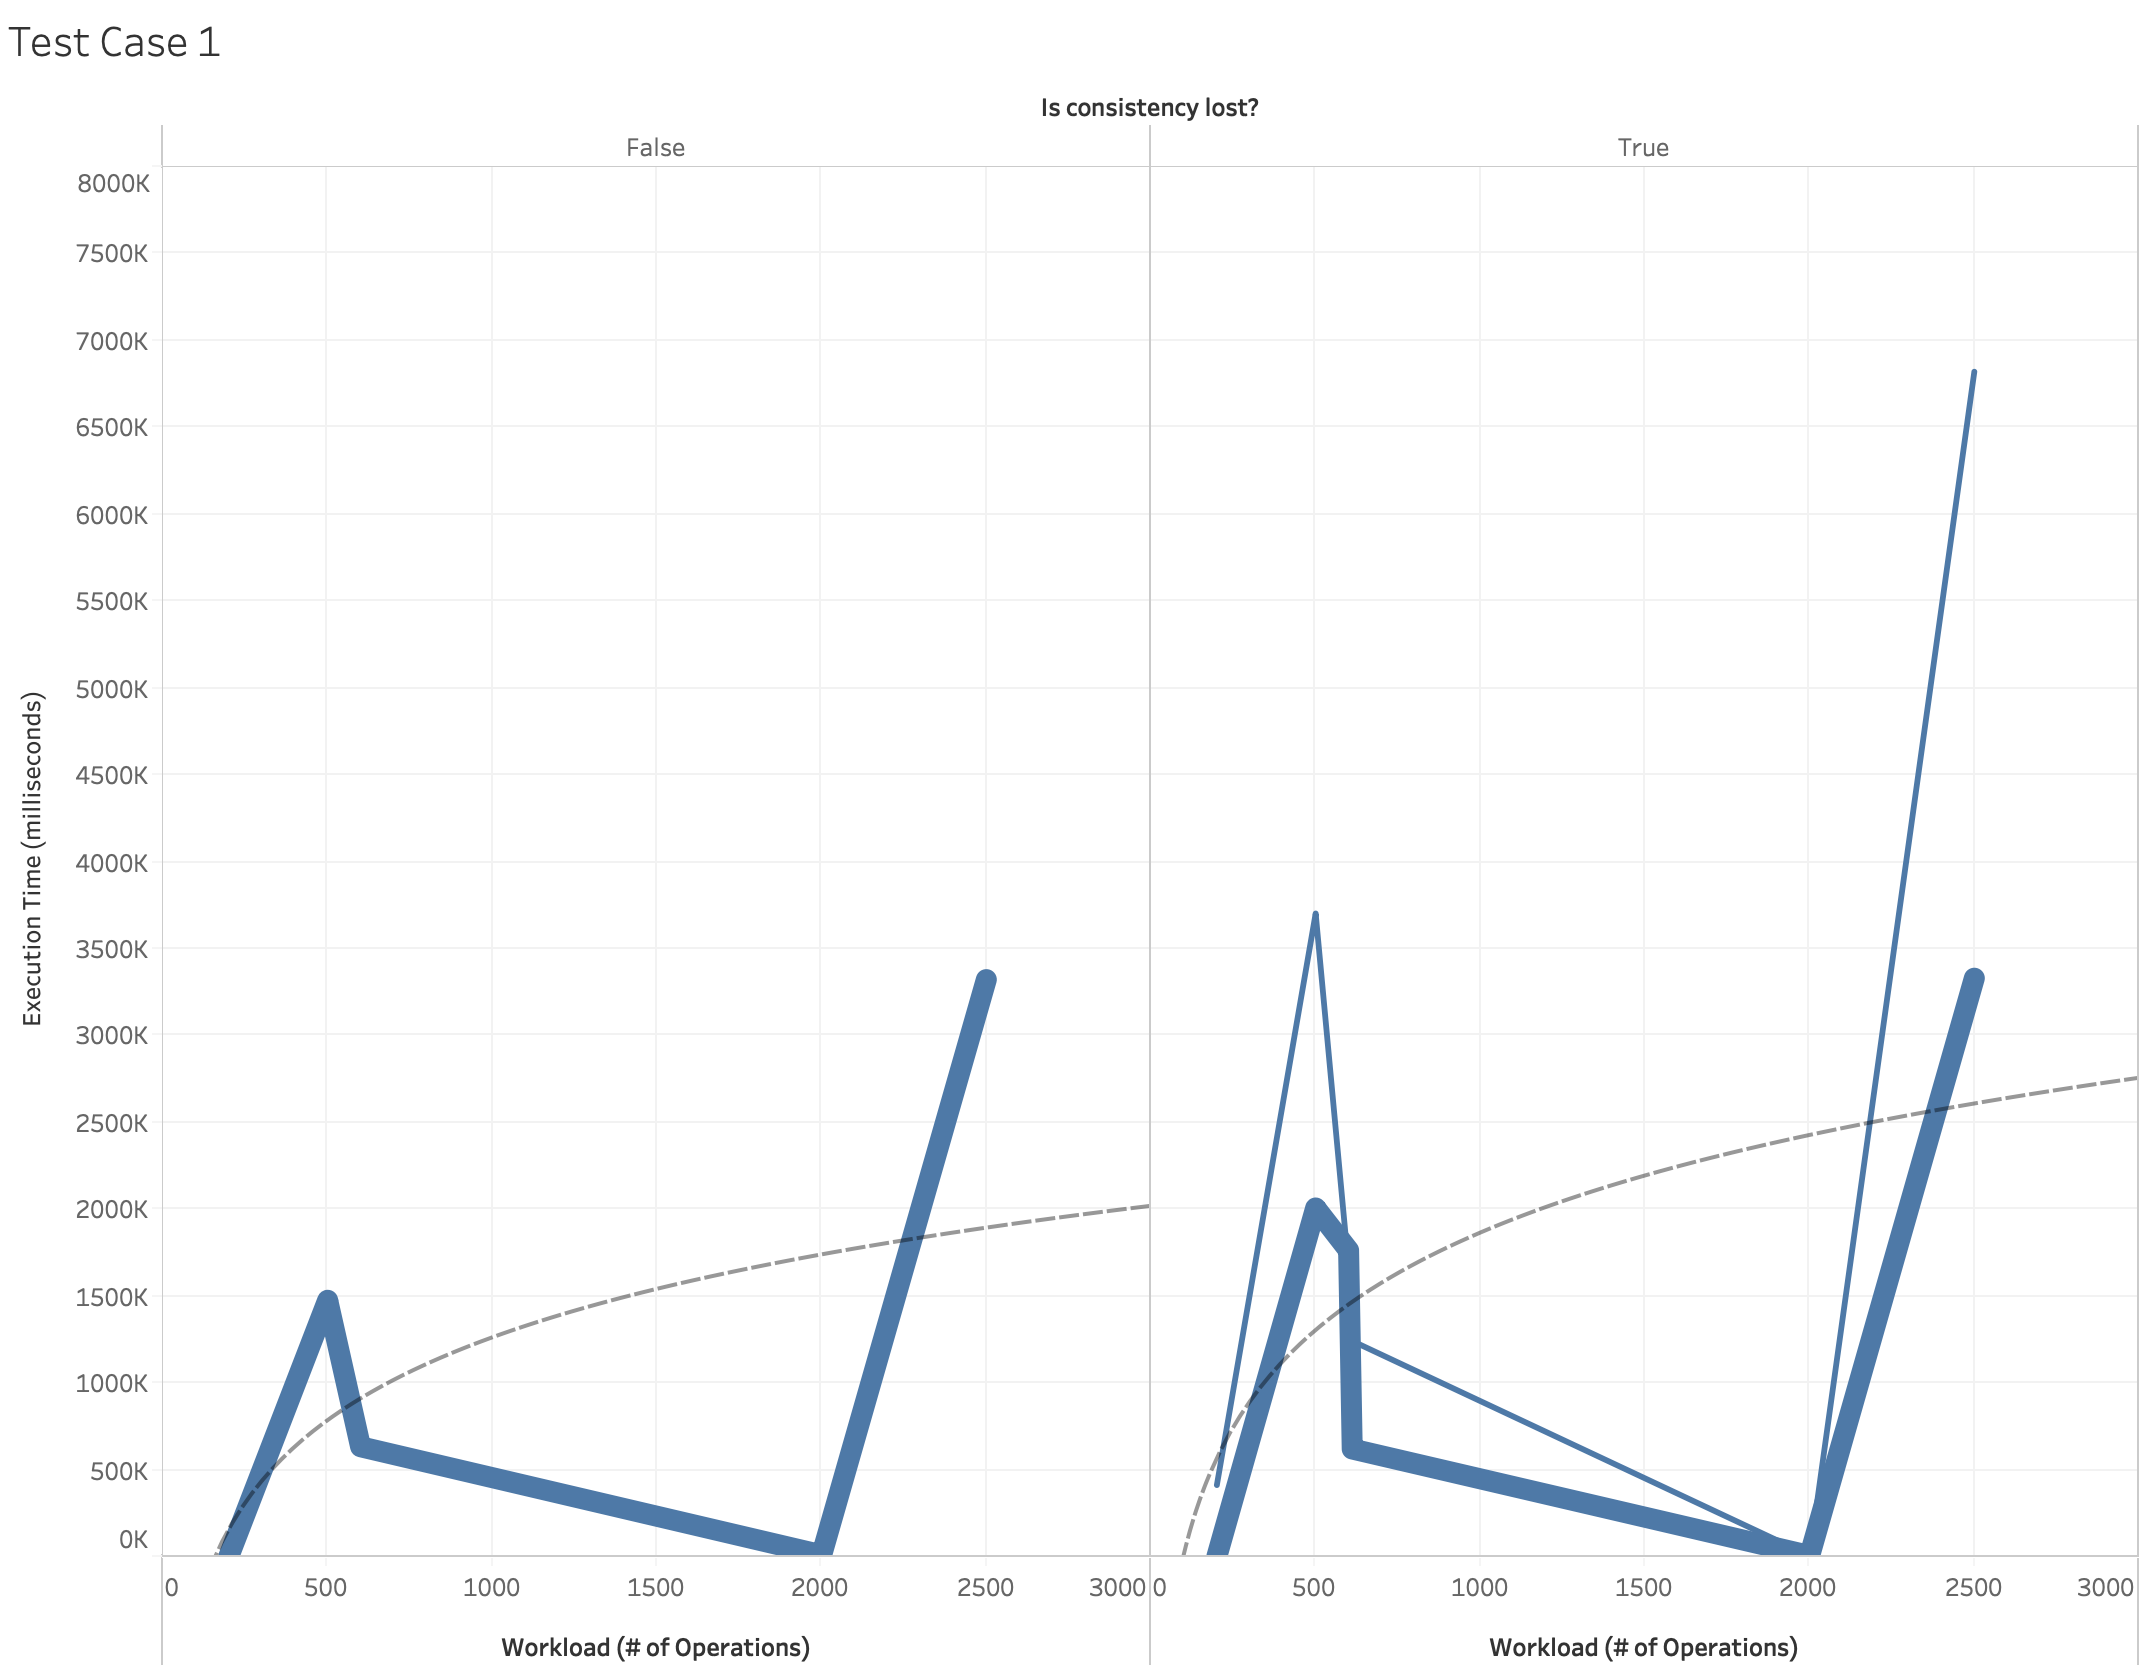
\includegraphics[scale=0.23]{images/TestCase1(WL).png}
\caption{Simulation Results for Test Case 1}
\label{results:test_case_graphs_1}
\end{figure}

\begin{figure}
\centering
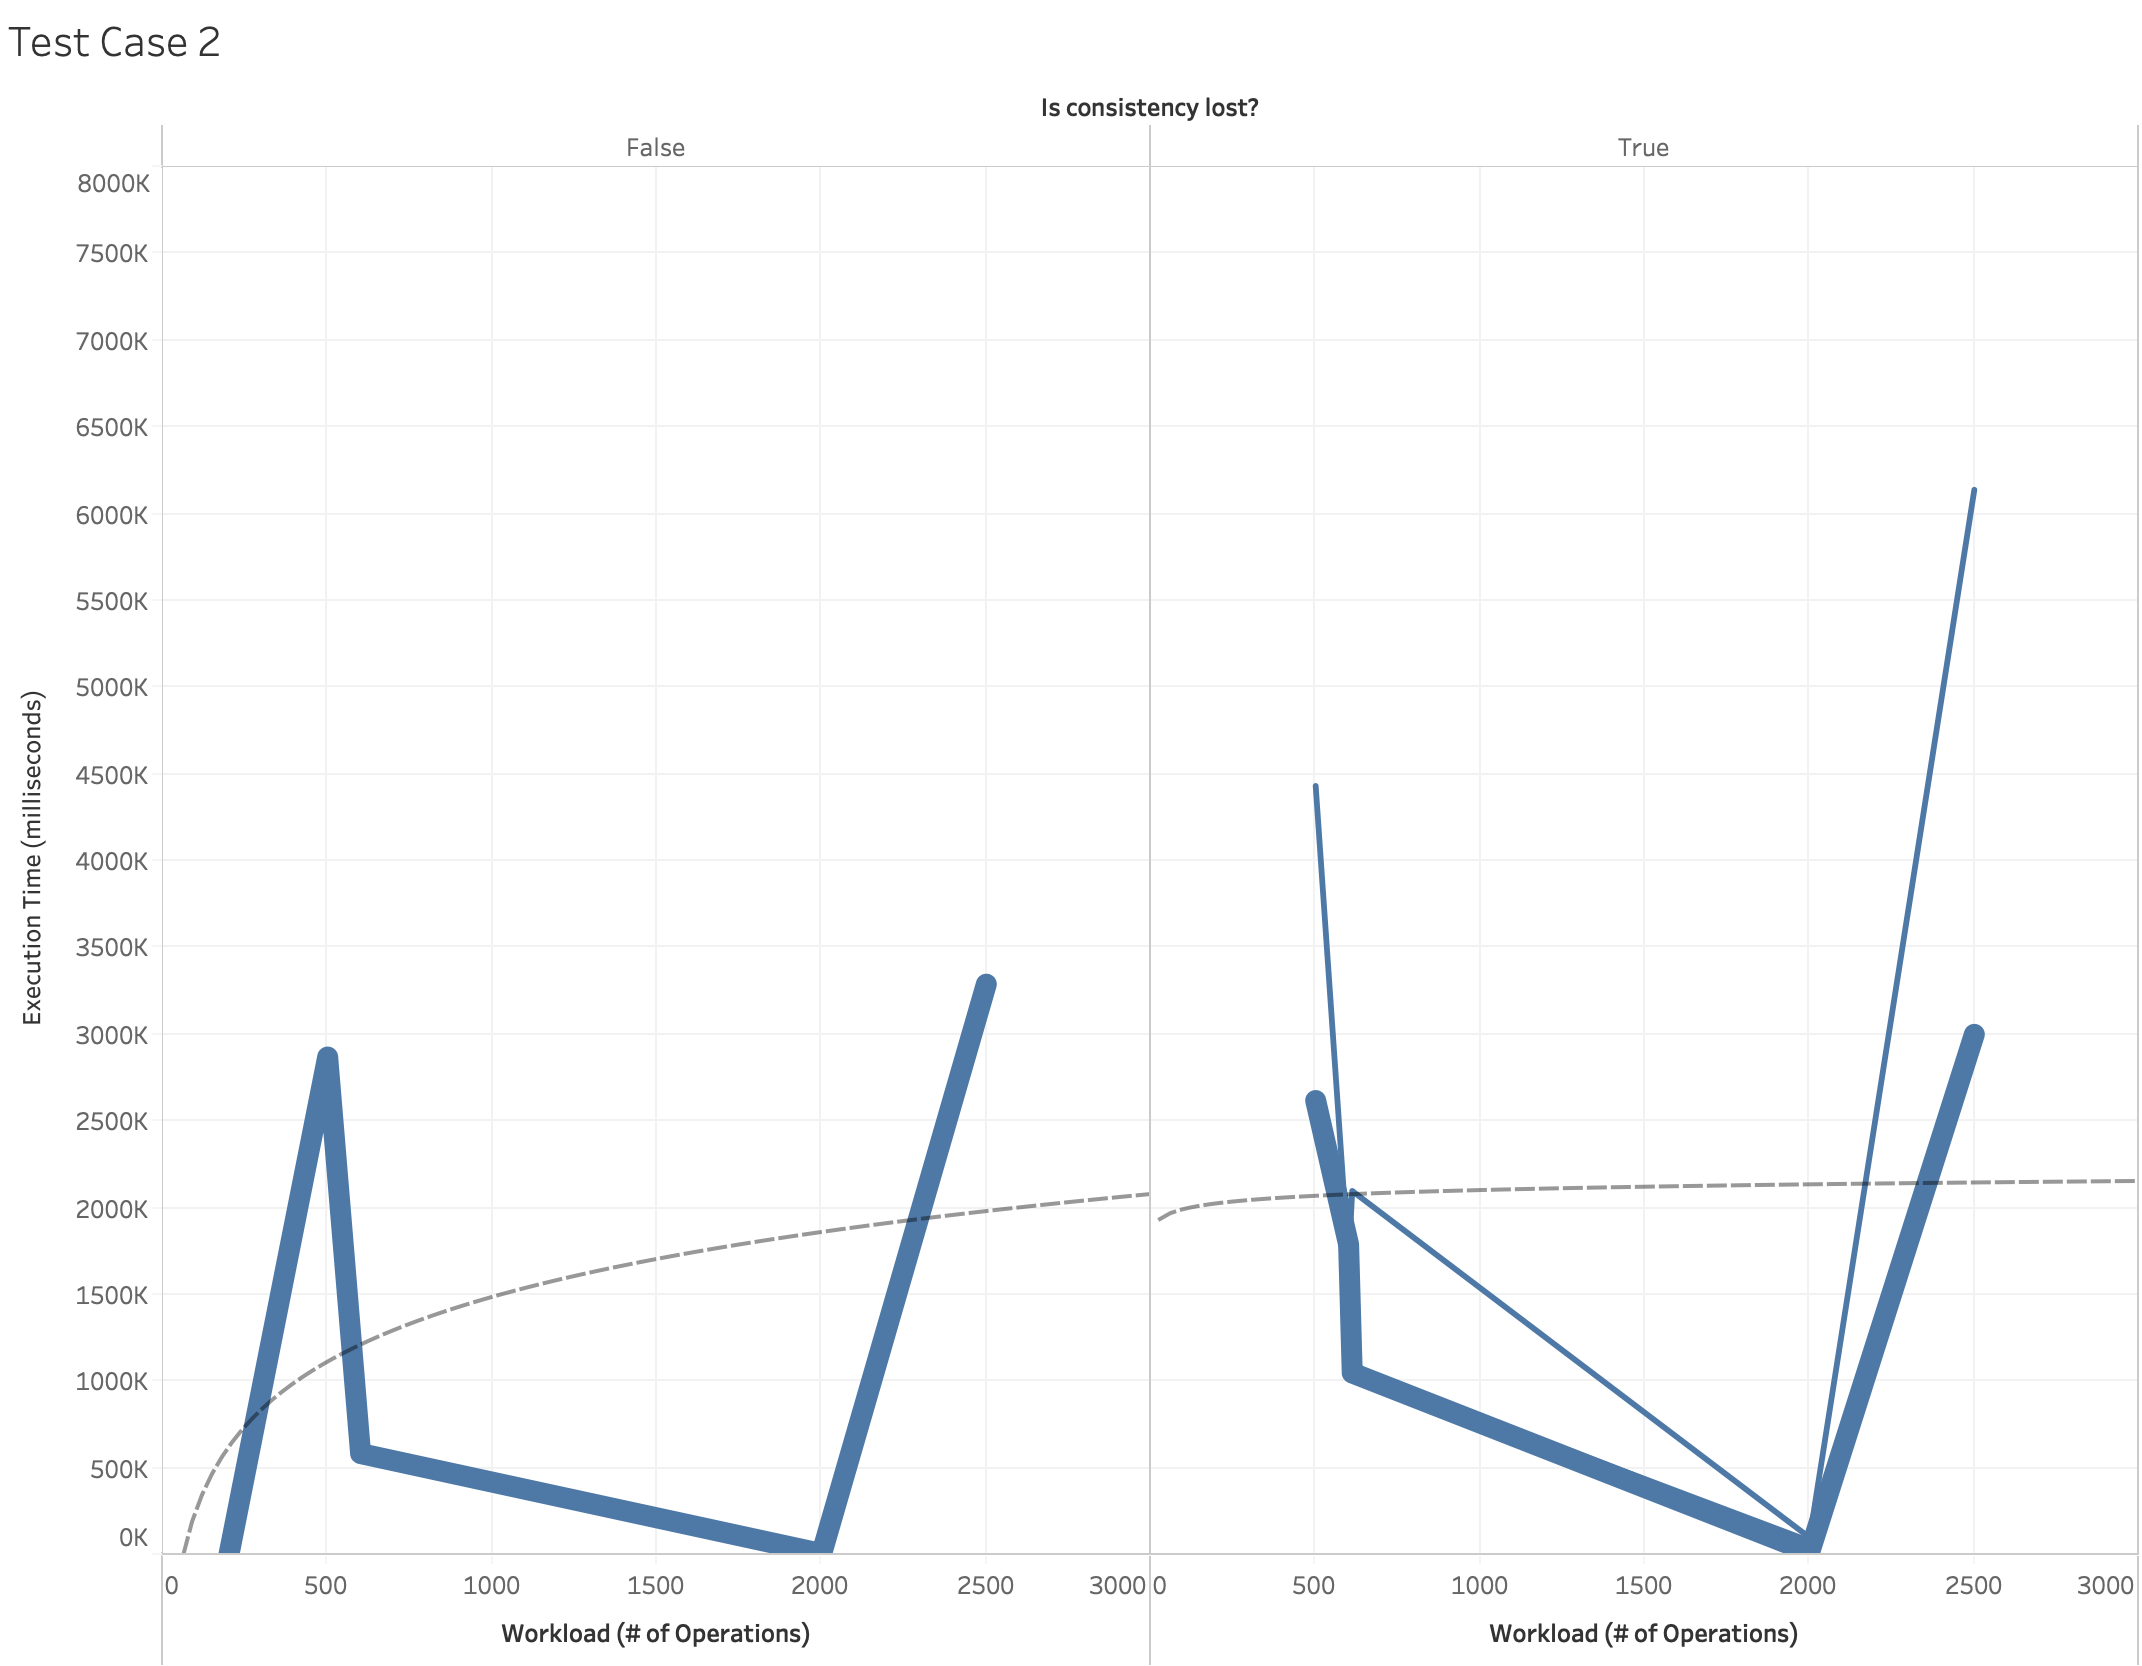
\includegraphics[scale=0.23]{images/TestCase2(WL).png}
\caption{Simulation Results for Test Case 2}
\label{results:test_case_graphs_2}
\end{figure}

\begin{figure}
\centering
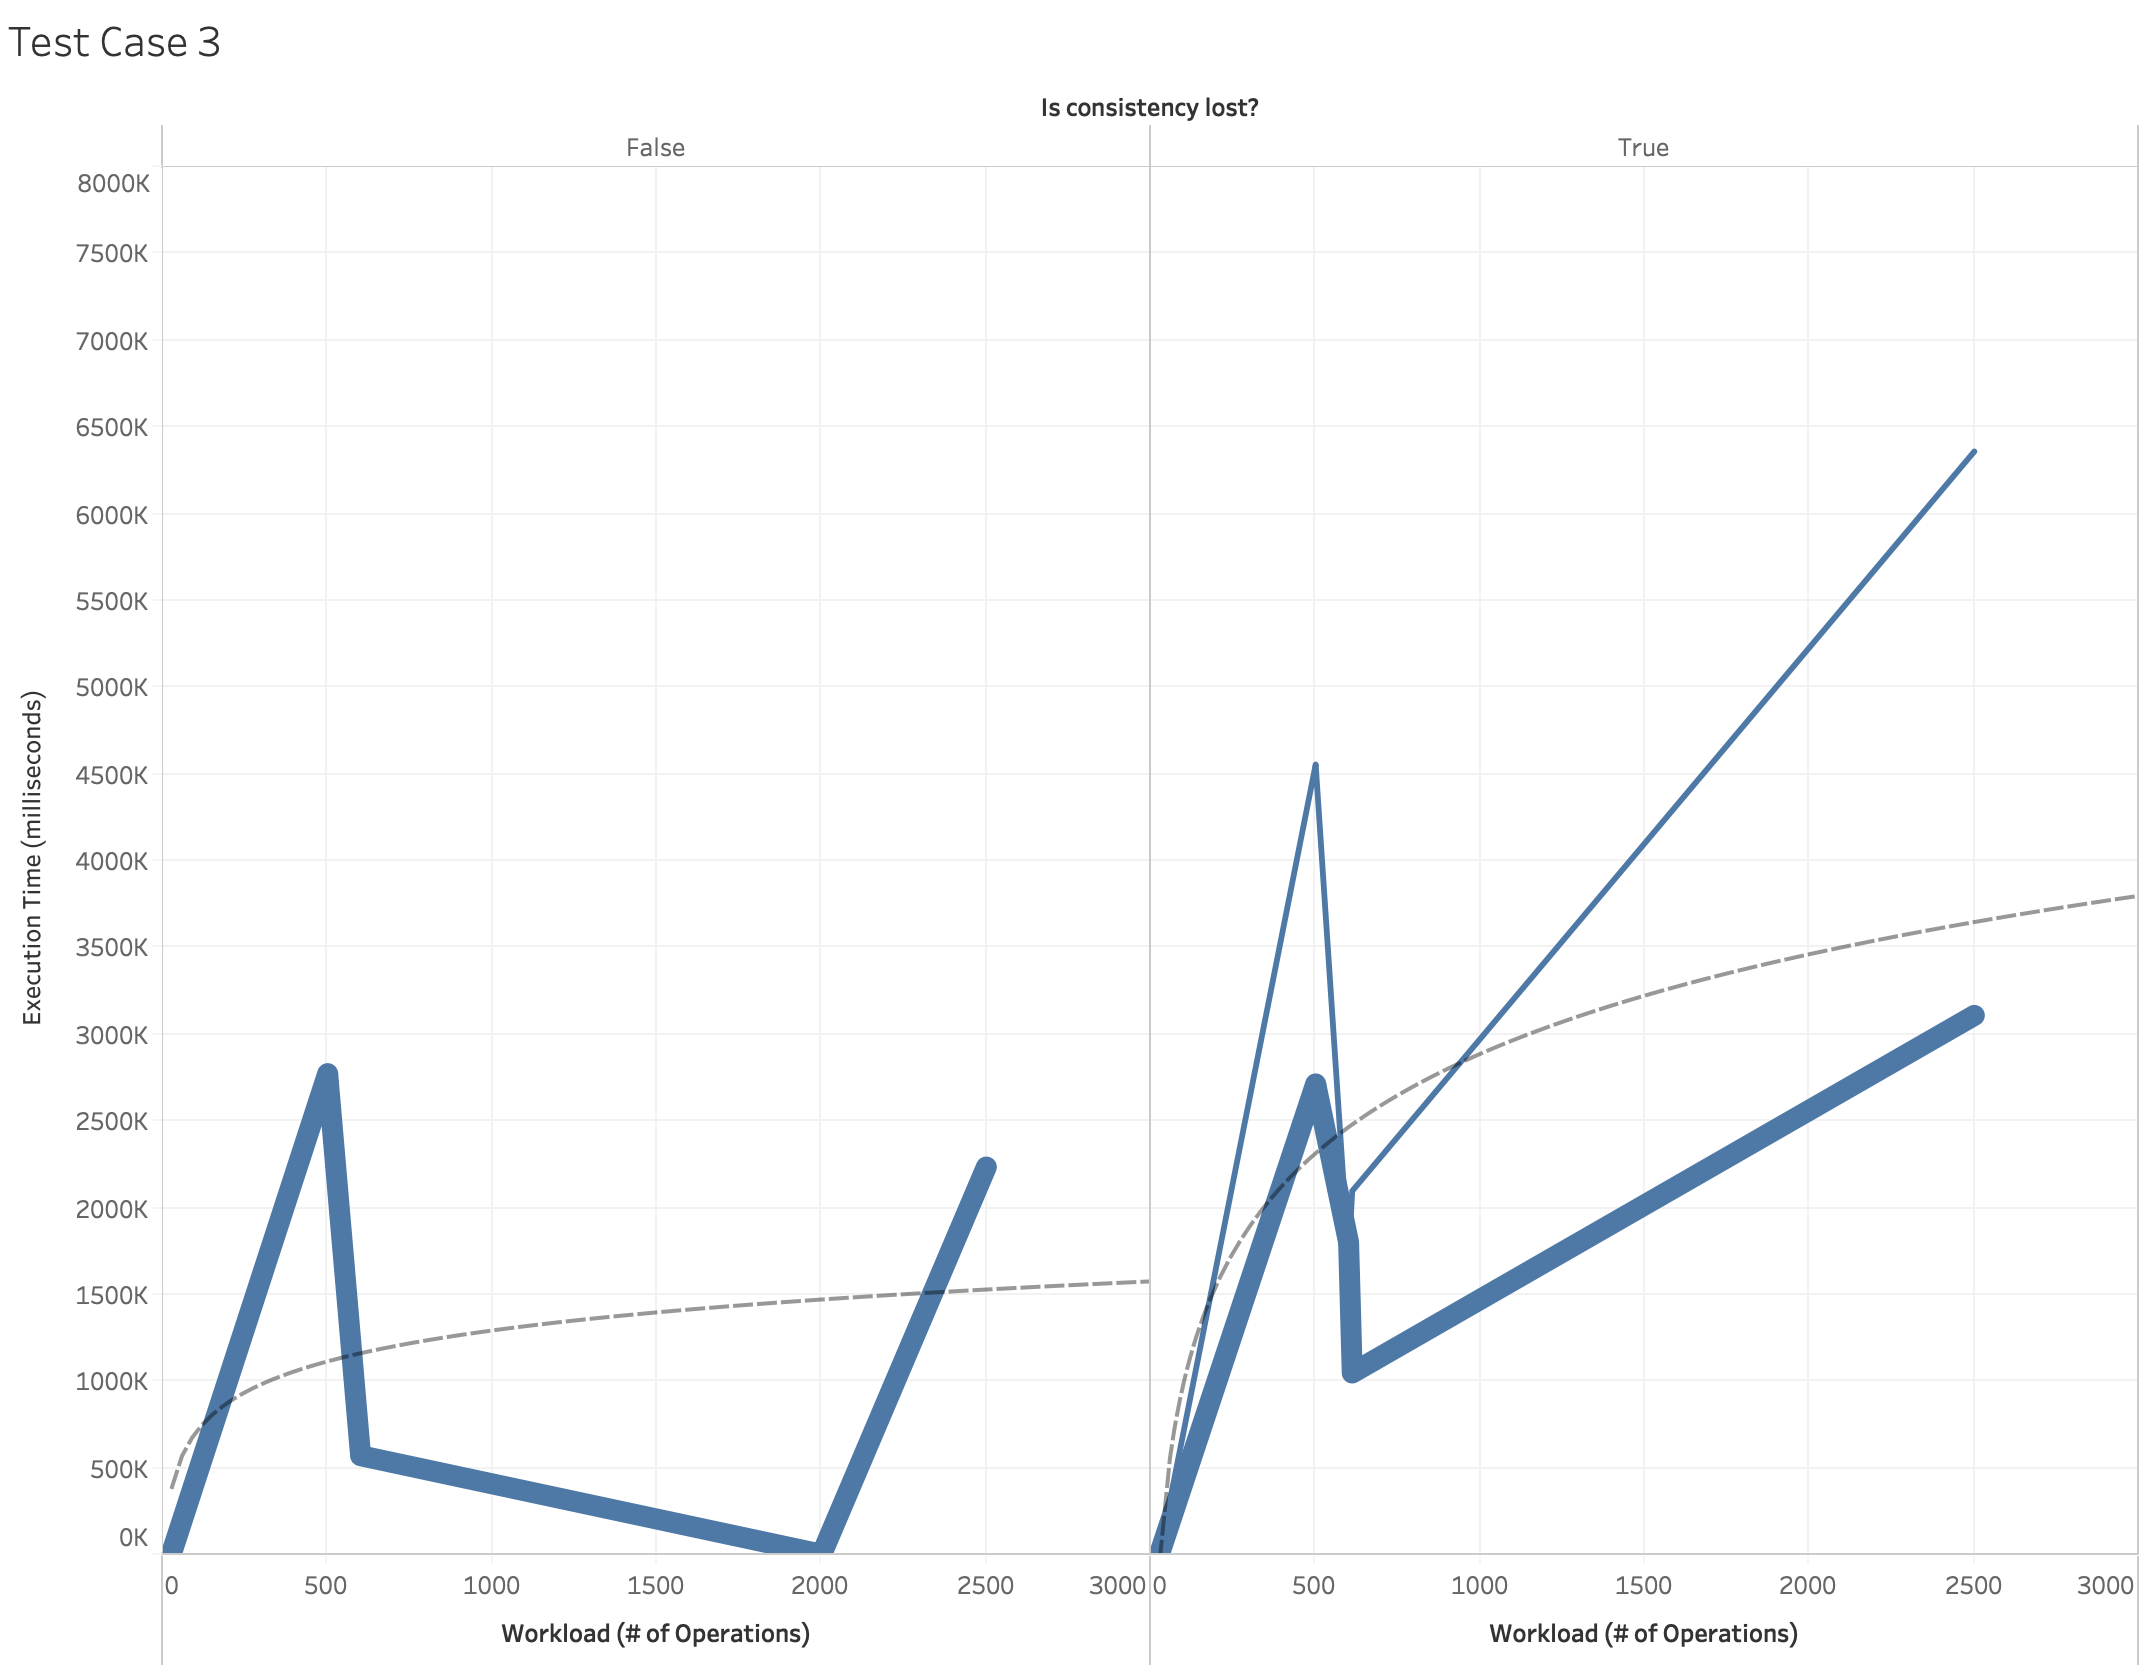
\includegraphics[scale=0.23]{images/TestCase3(WL).png}
\caption{Simulation Results for Test Case 3}
\label{results:test_case_graphs_3}
\end{figure}

\begin{figure}
\centering
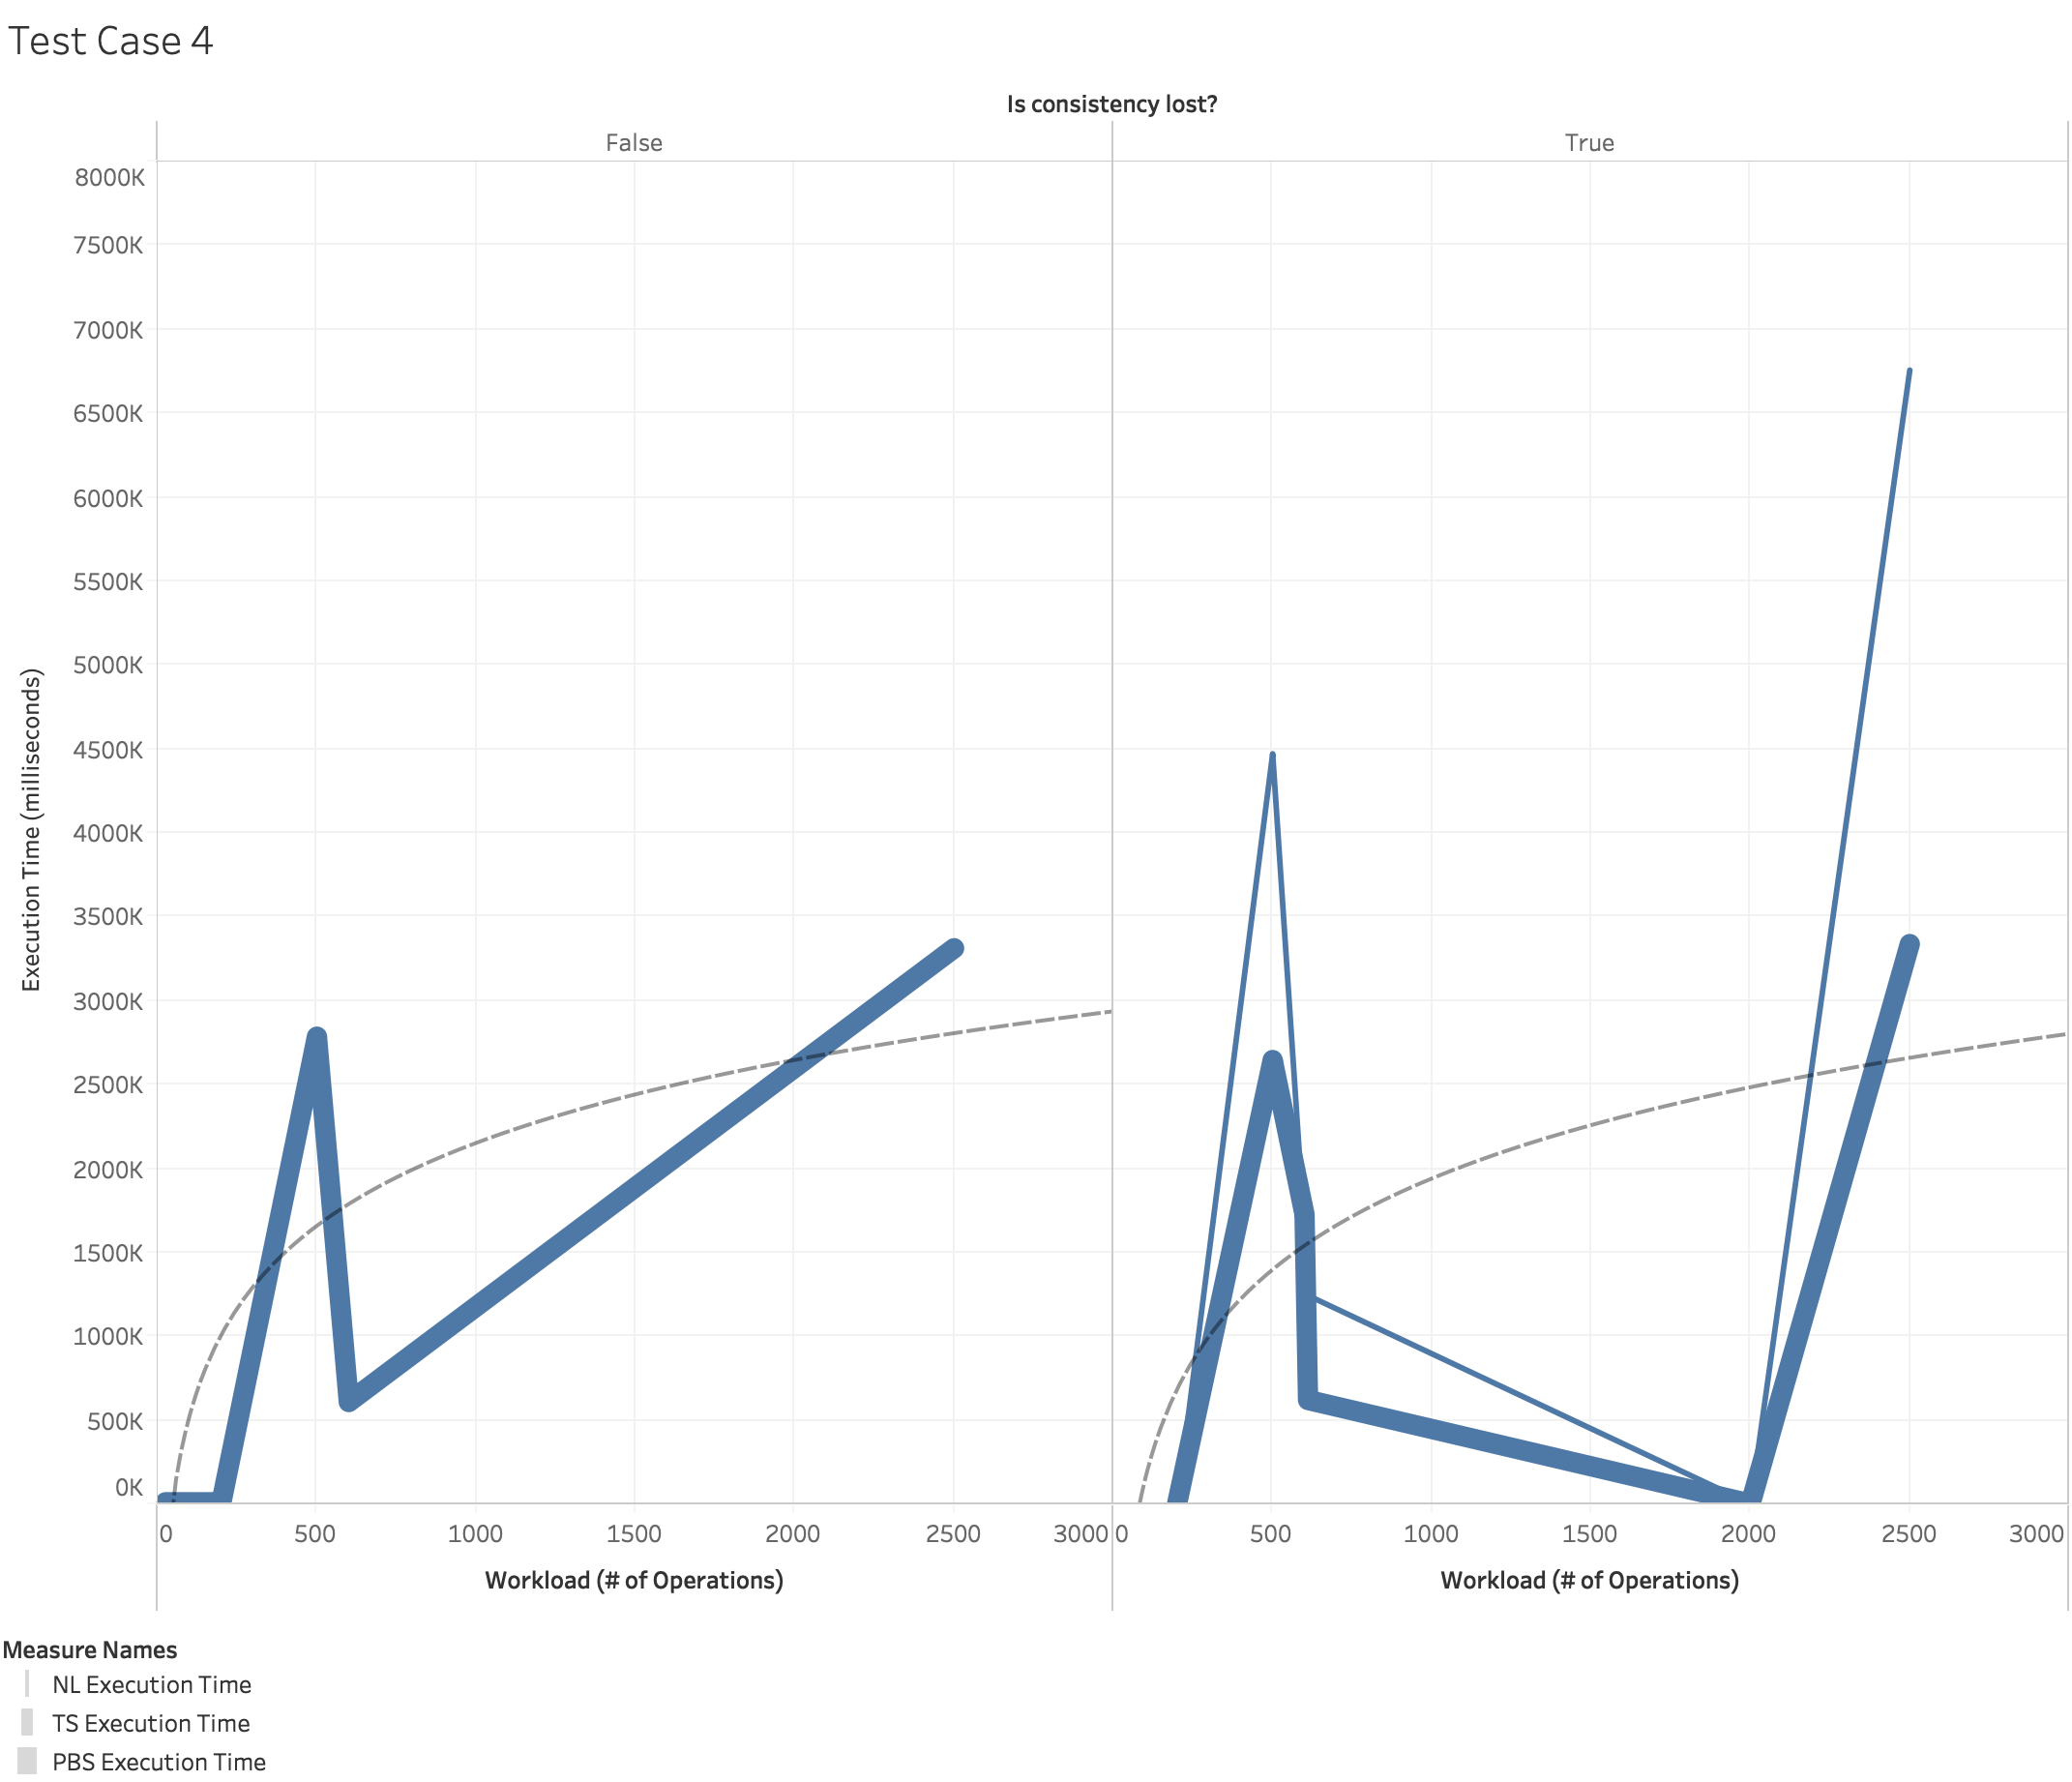
\includegraphics[scale=0.23]{images/TestCase4(WL).png}
\caption{Simulation Results for Test Case 4}
\label{results:test_case_graphs_4}
\end{figure}

\begin{figure}
\centering
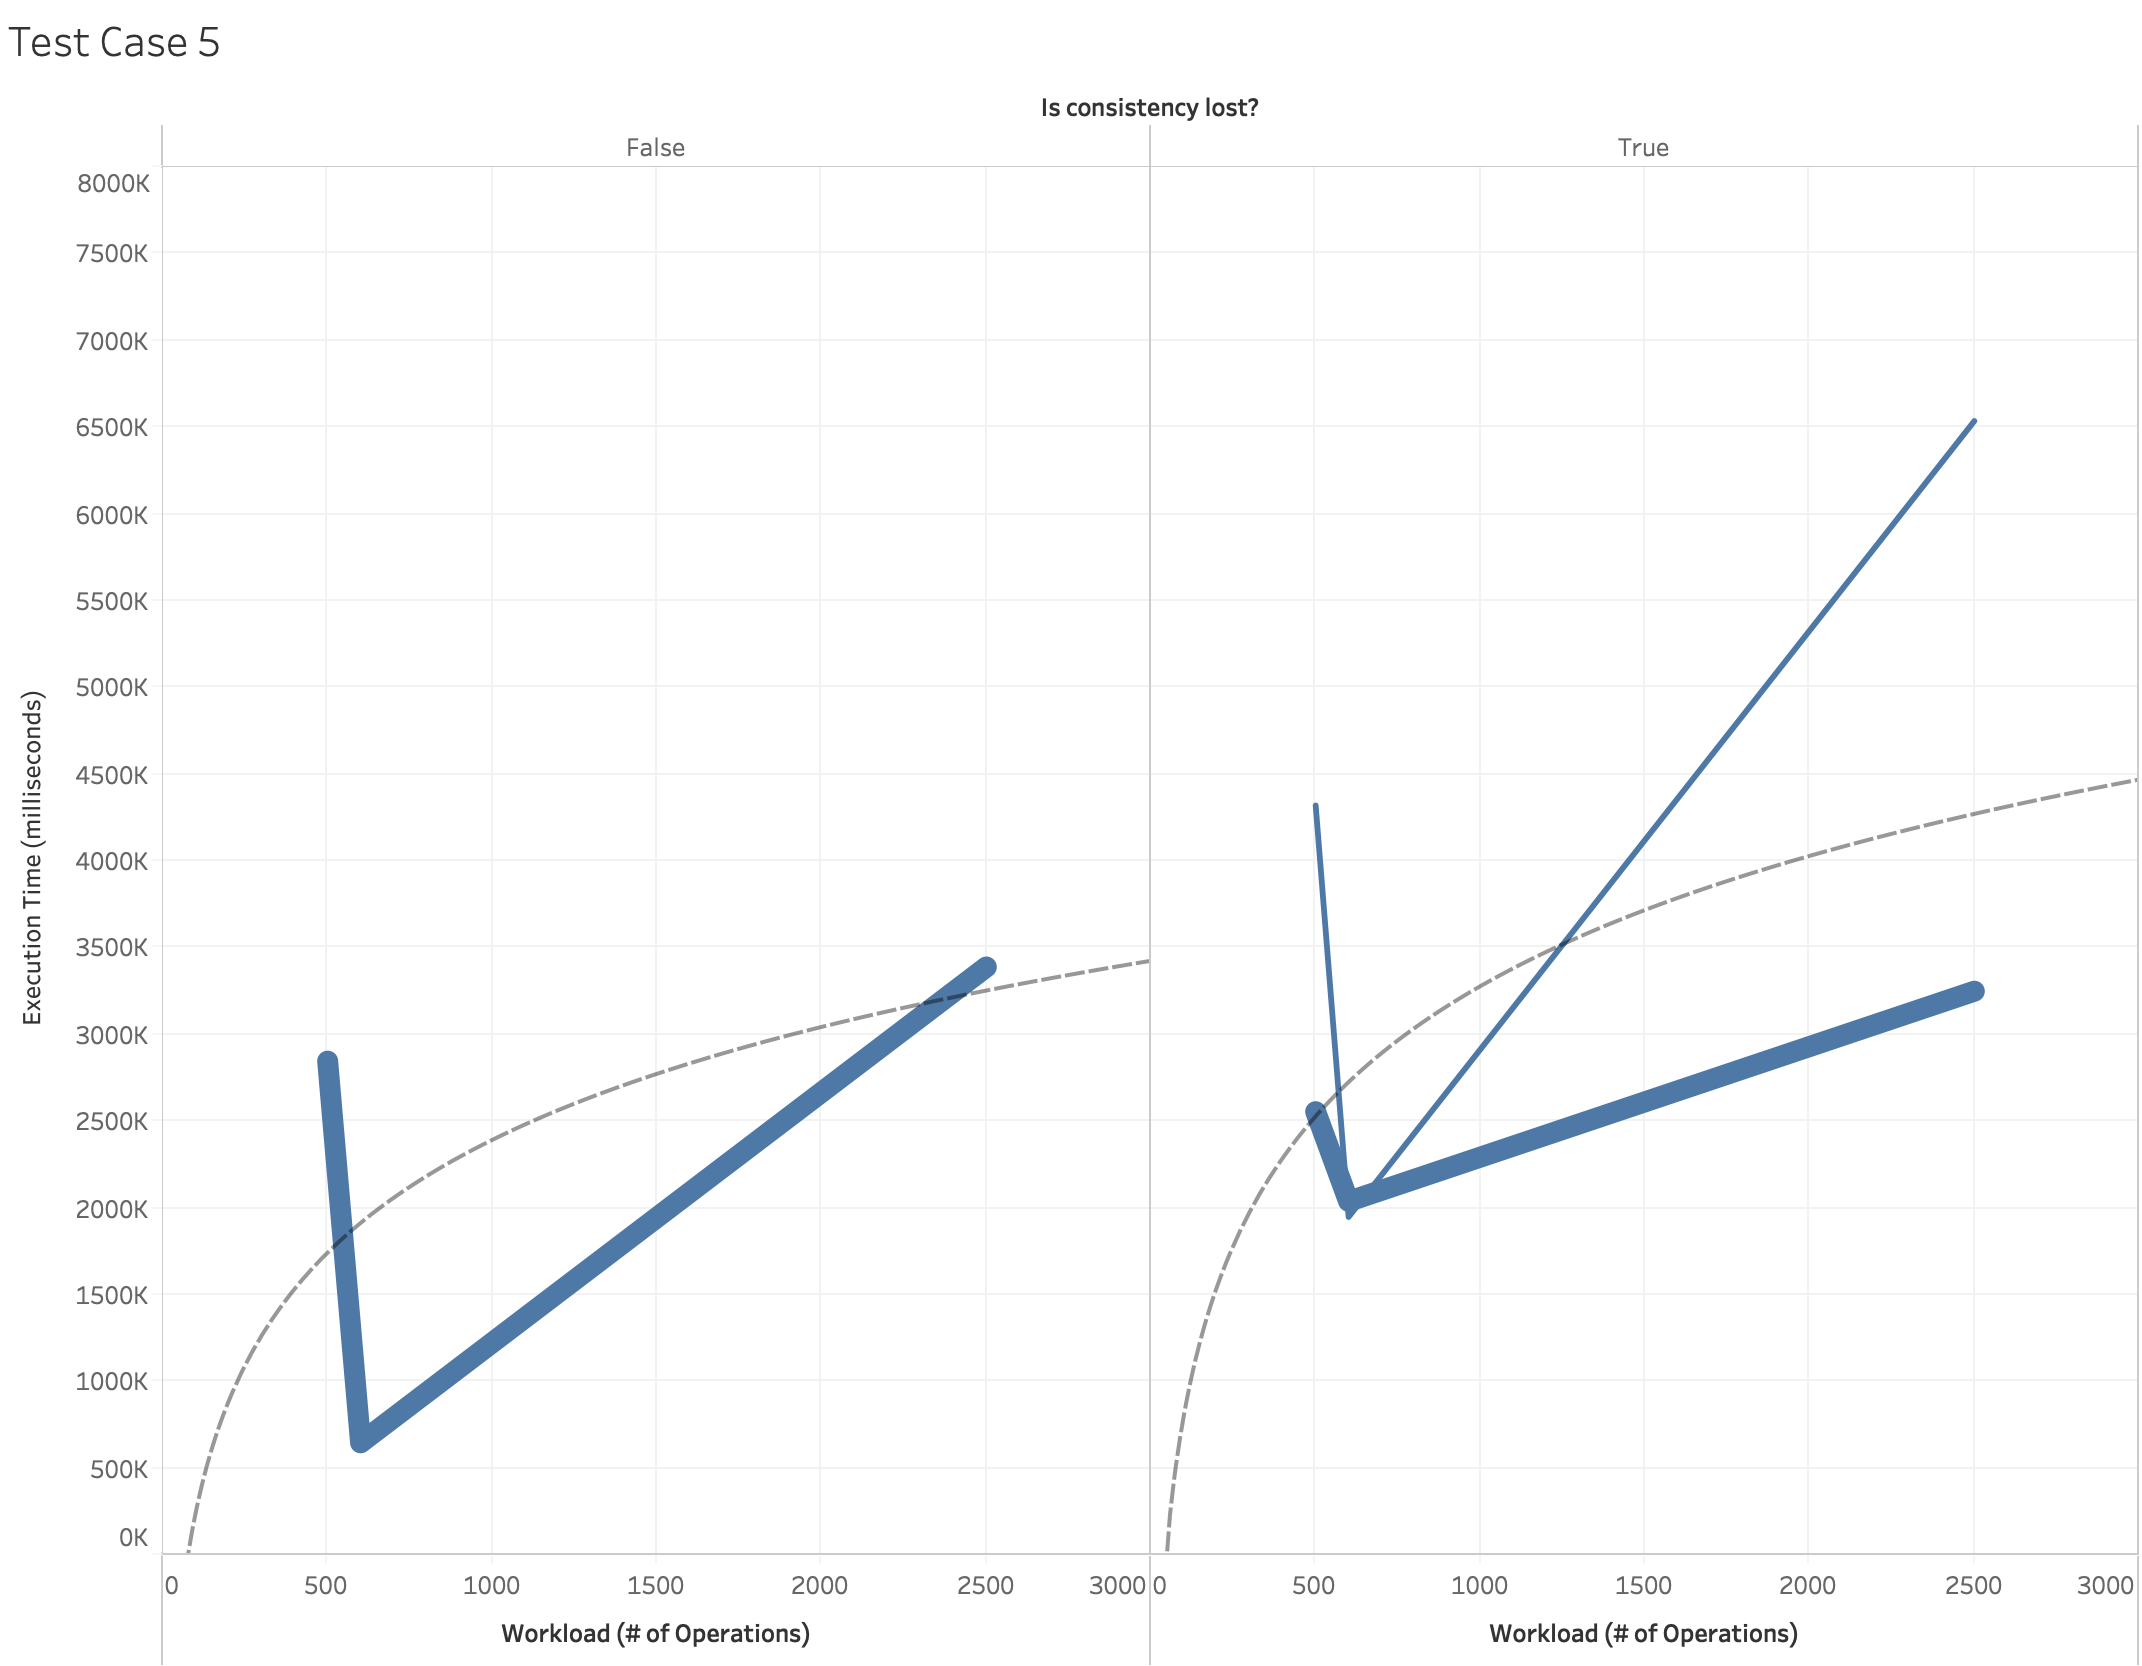
\includegraphics[scale=0.23]{images/TestCase5(WL).png}
\caption{Simulation Results for Test Case 5}
\label{results:test_case_graphs_5}
\end{figure}

\begin{figure}
\centering
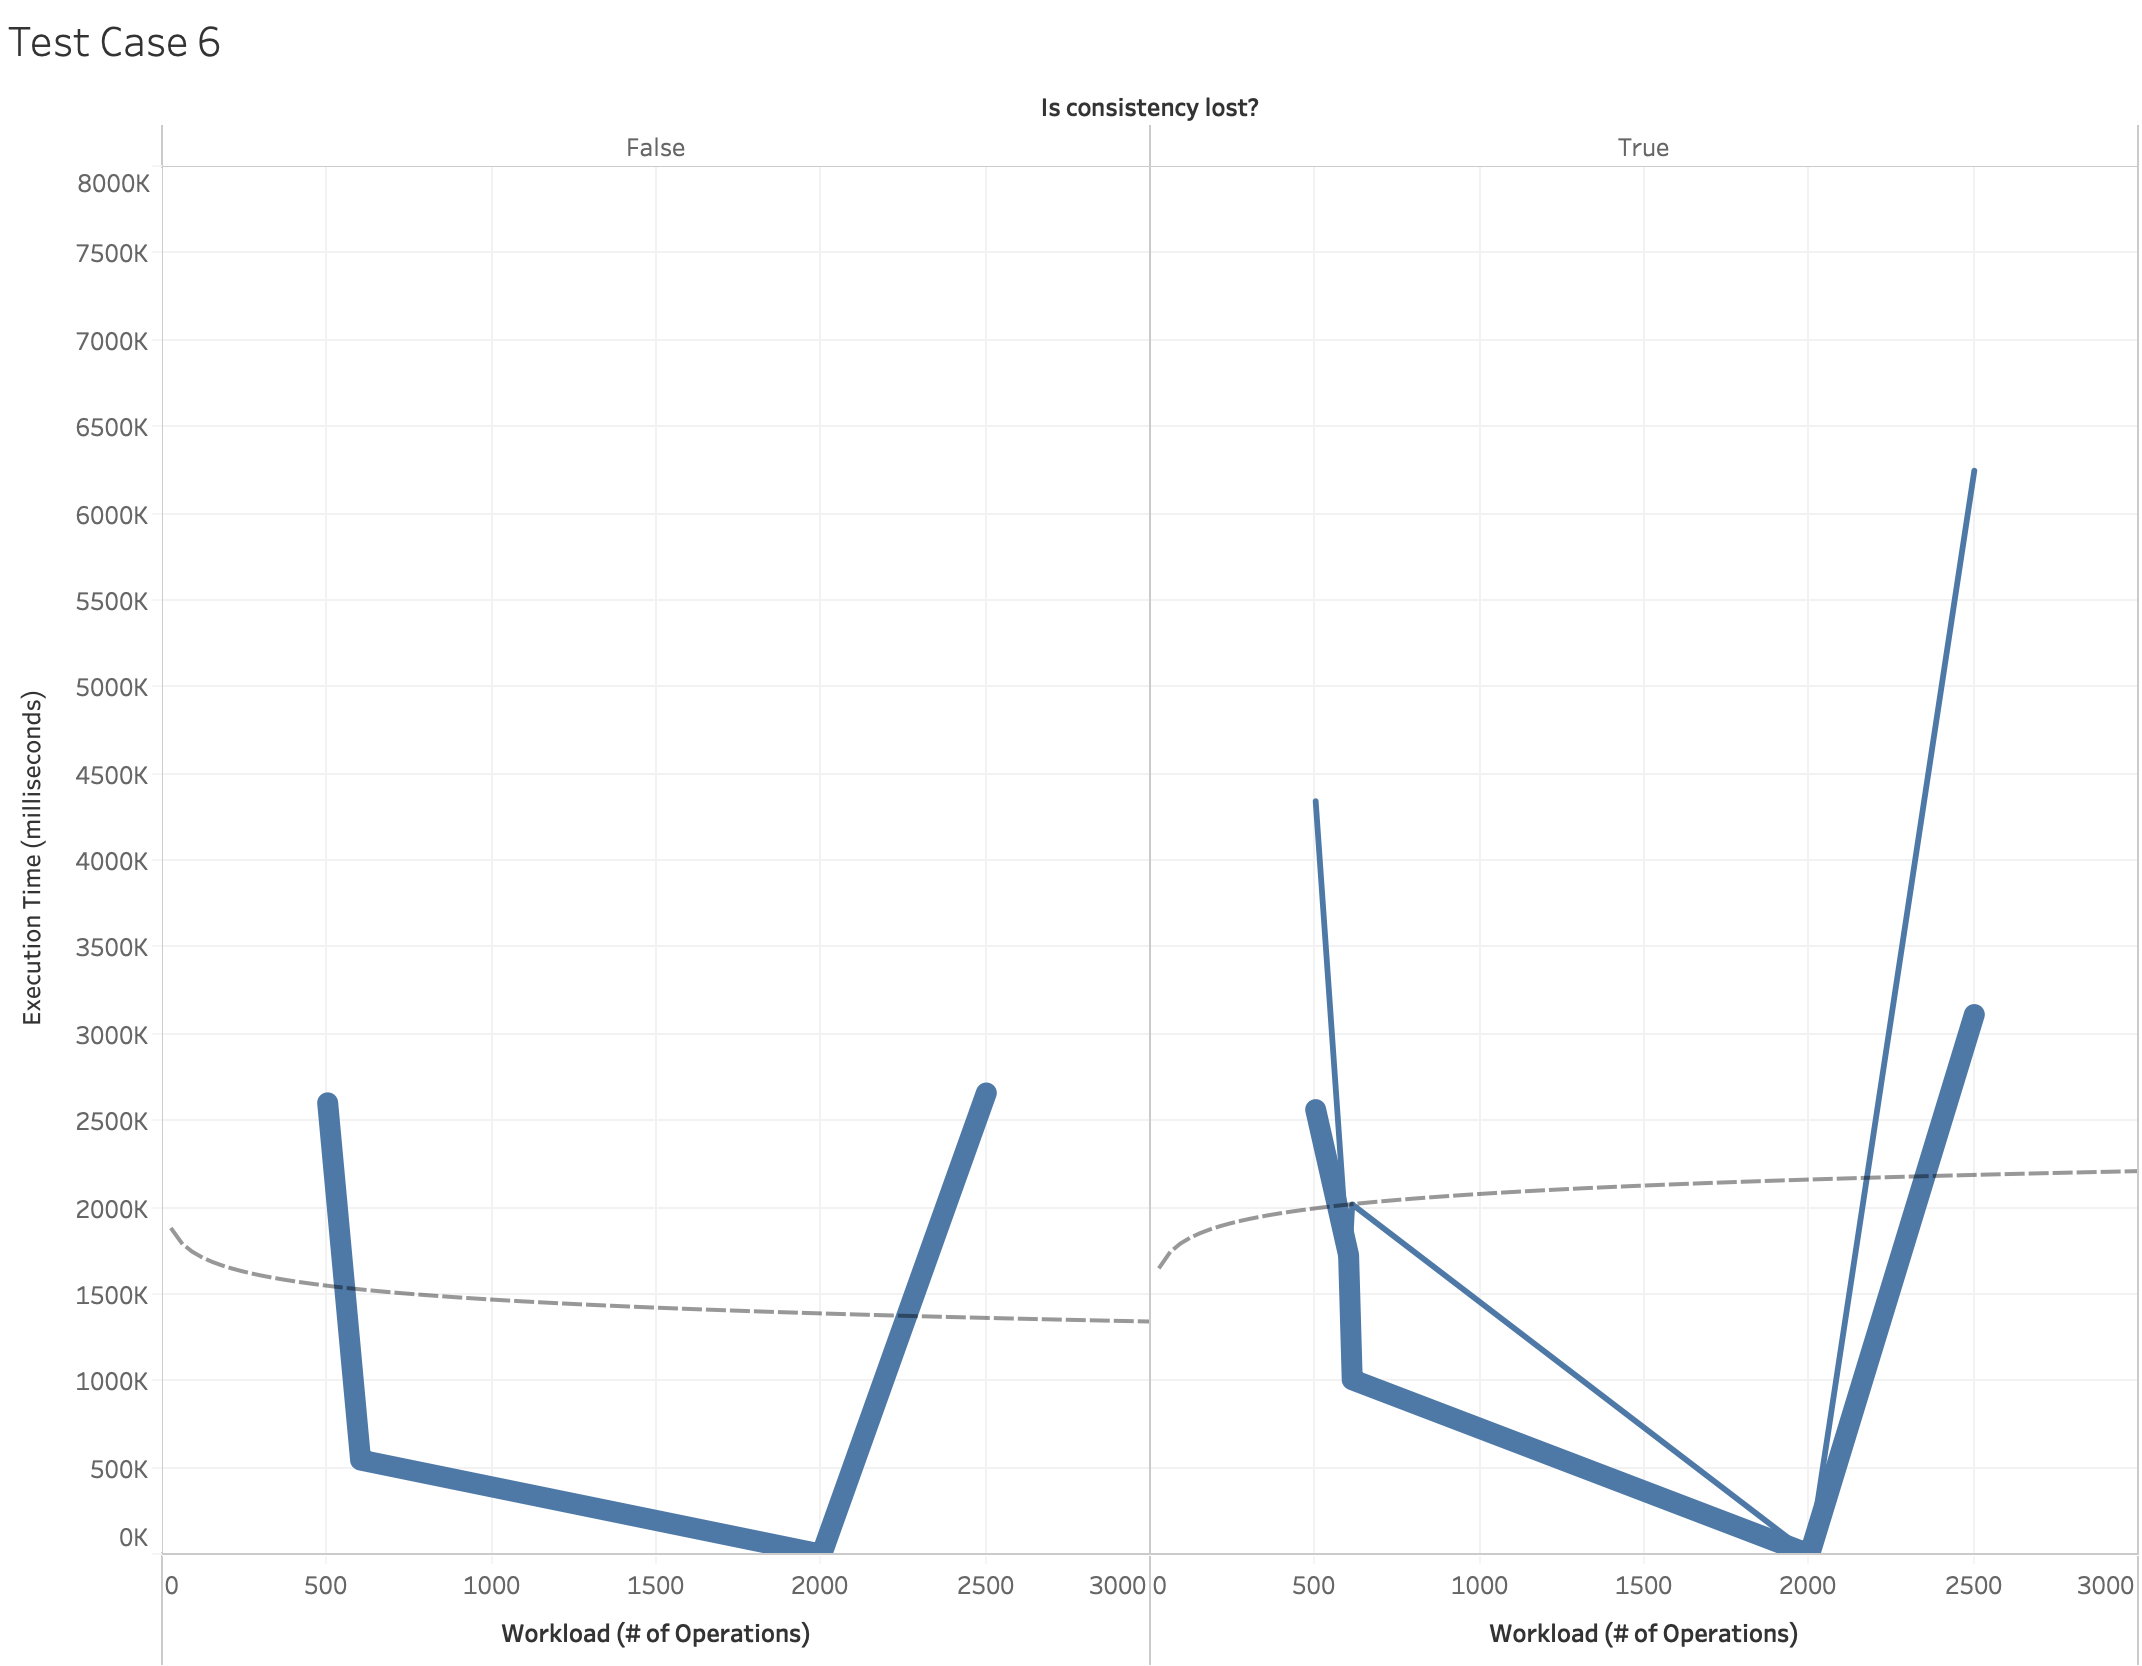
\includegraphics[scale=0.20]{images/TestCase6(WL).png}
\caption{Simulation Results for Test Case 6}
\label{results:test_case_graphs_6}
\end{figure}

\begin{figure}
\centering
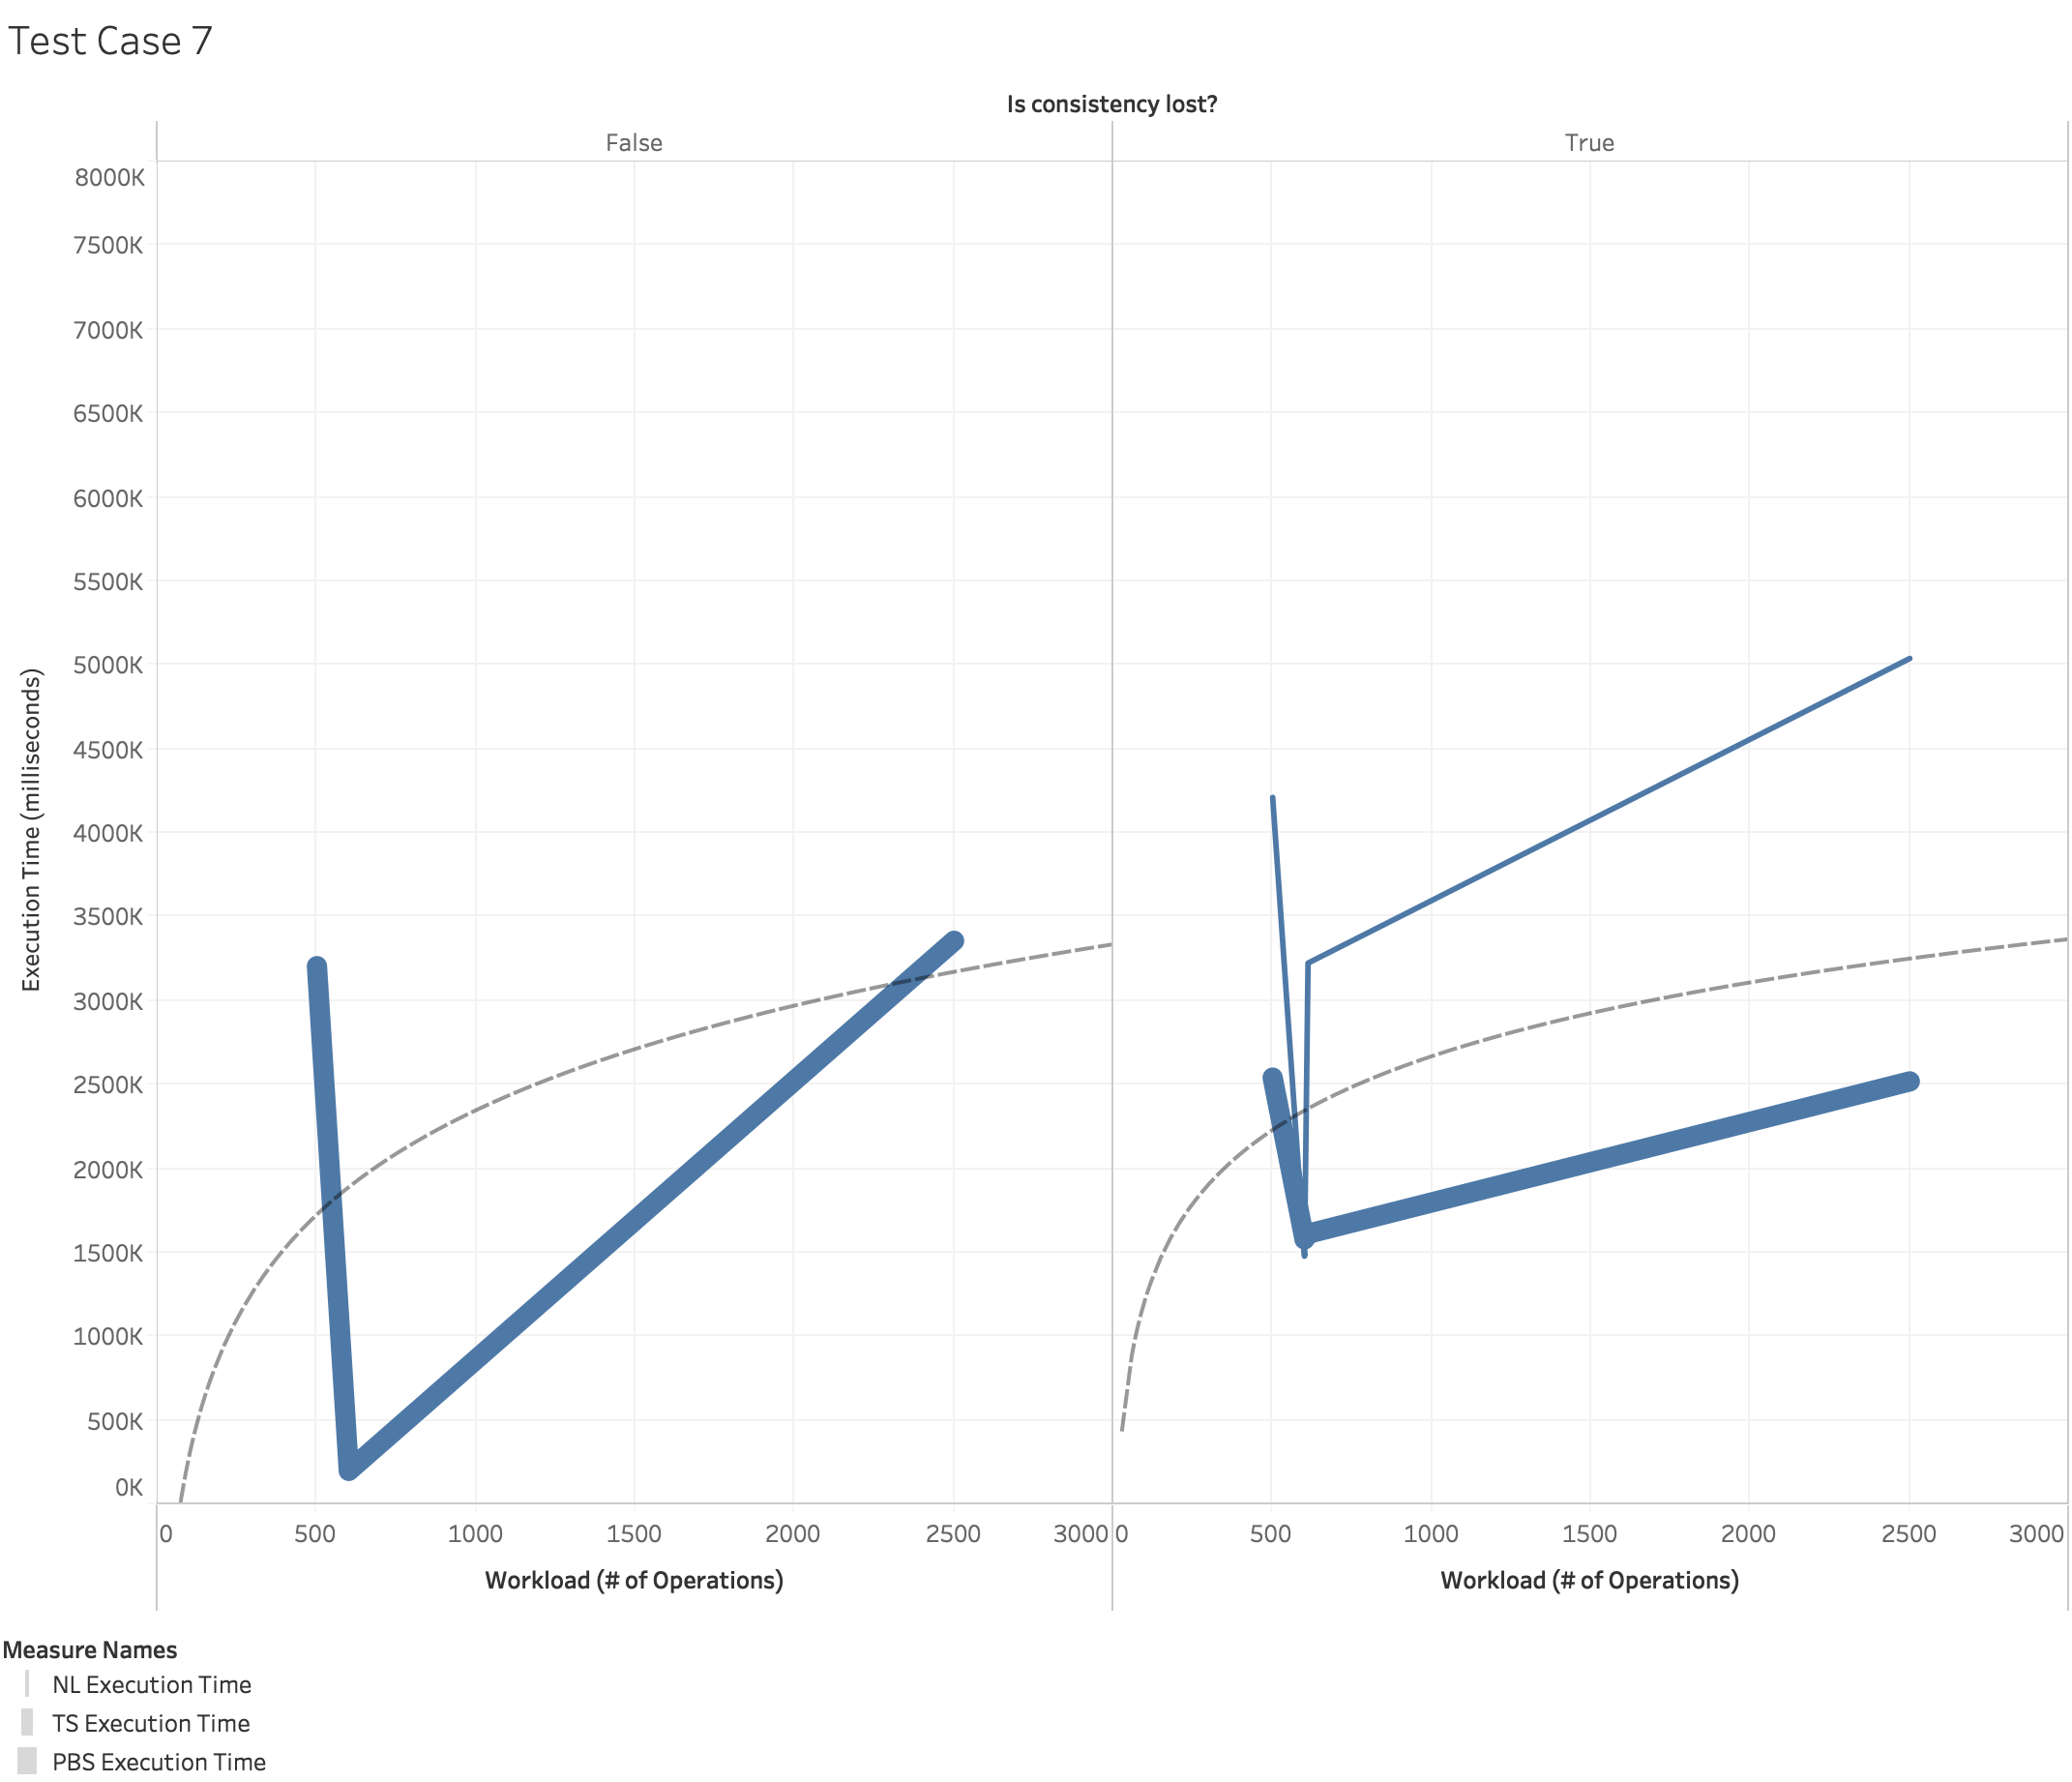
\includegraphics[scale=0.20]{images/TestCase7(WL).png}
\caption{Simulation Results for Test Case 7}
\label{results:test_case_graphs_7}
\end{figure}

\begin{figure}
\centering
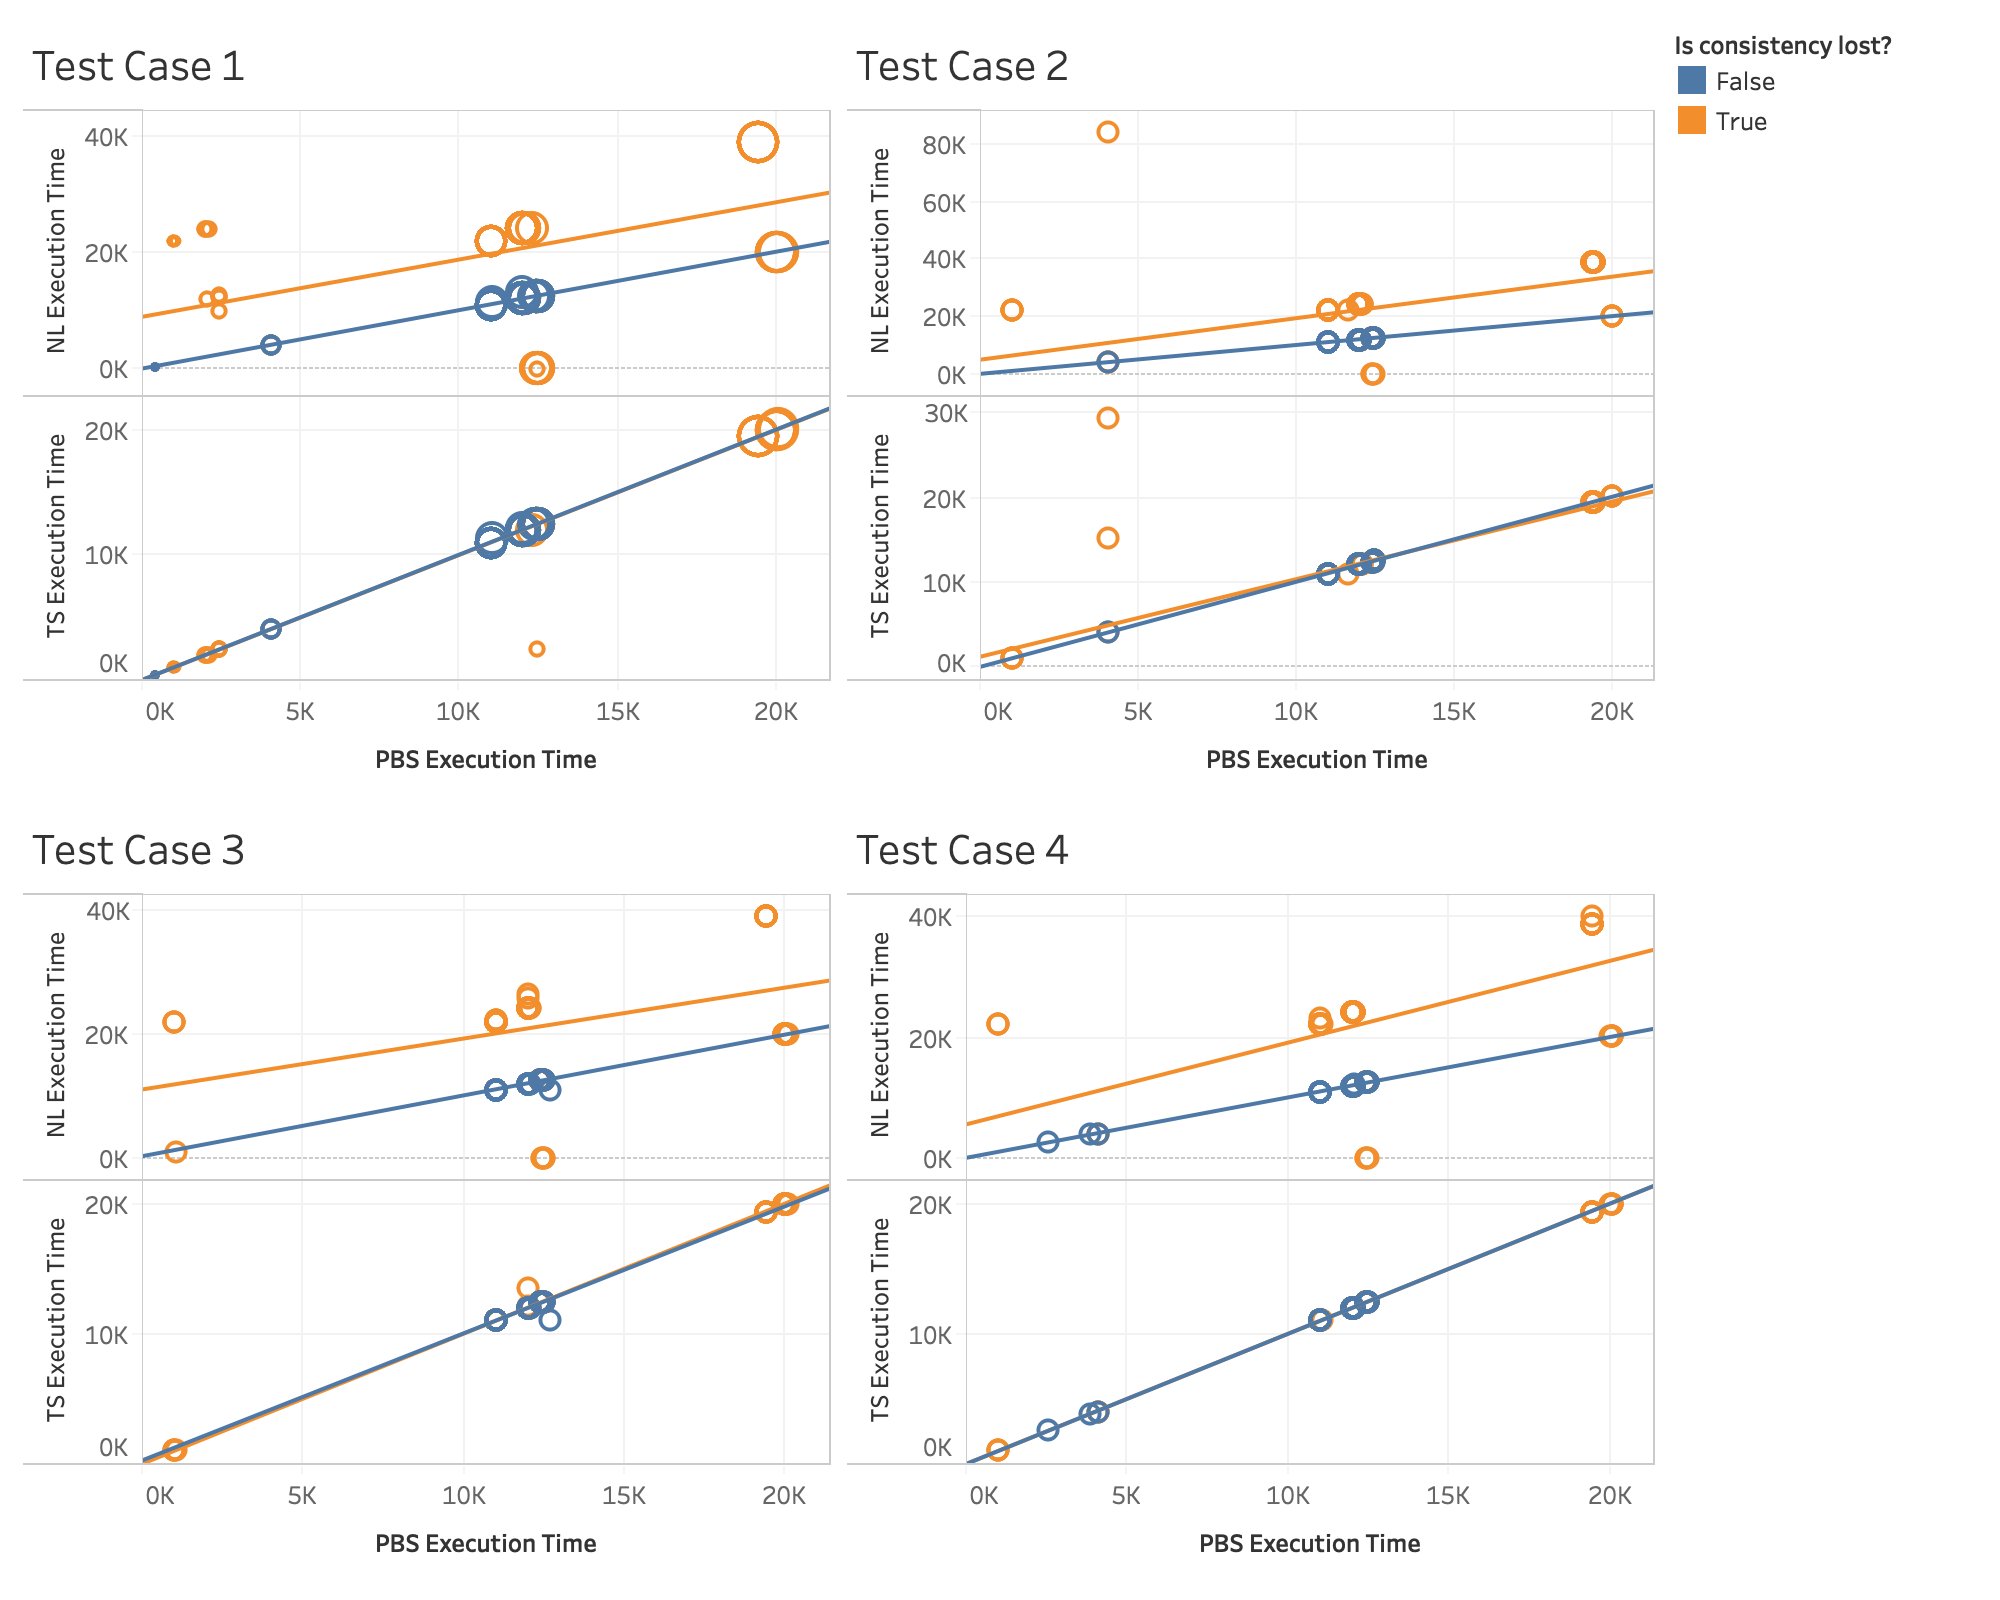
\includegraphics[scale=0.25]{images/Dashboard1_TL.png}
\caption{Consistency Lost/Kept for Test Cases 1-4}
\label{results:consistency_test_case_graphs_1_4}
\end{figure}

\begin{figure}
\centering
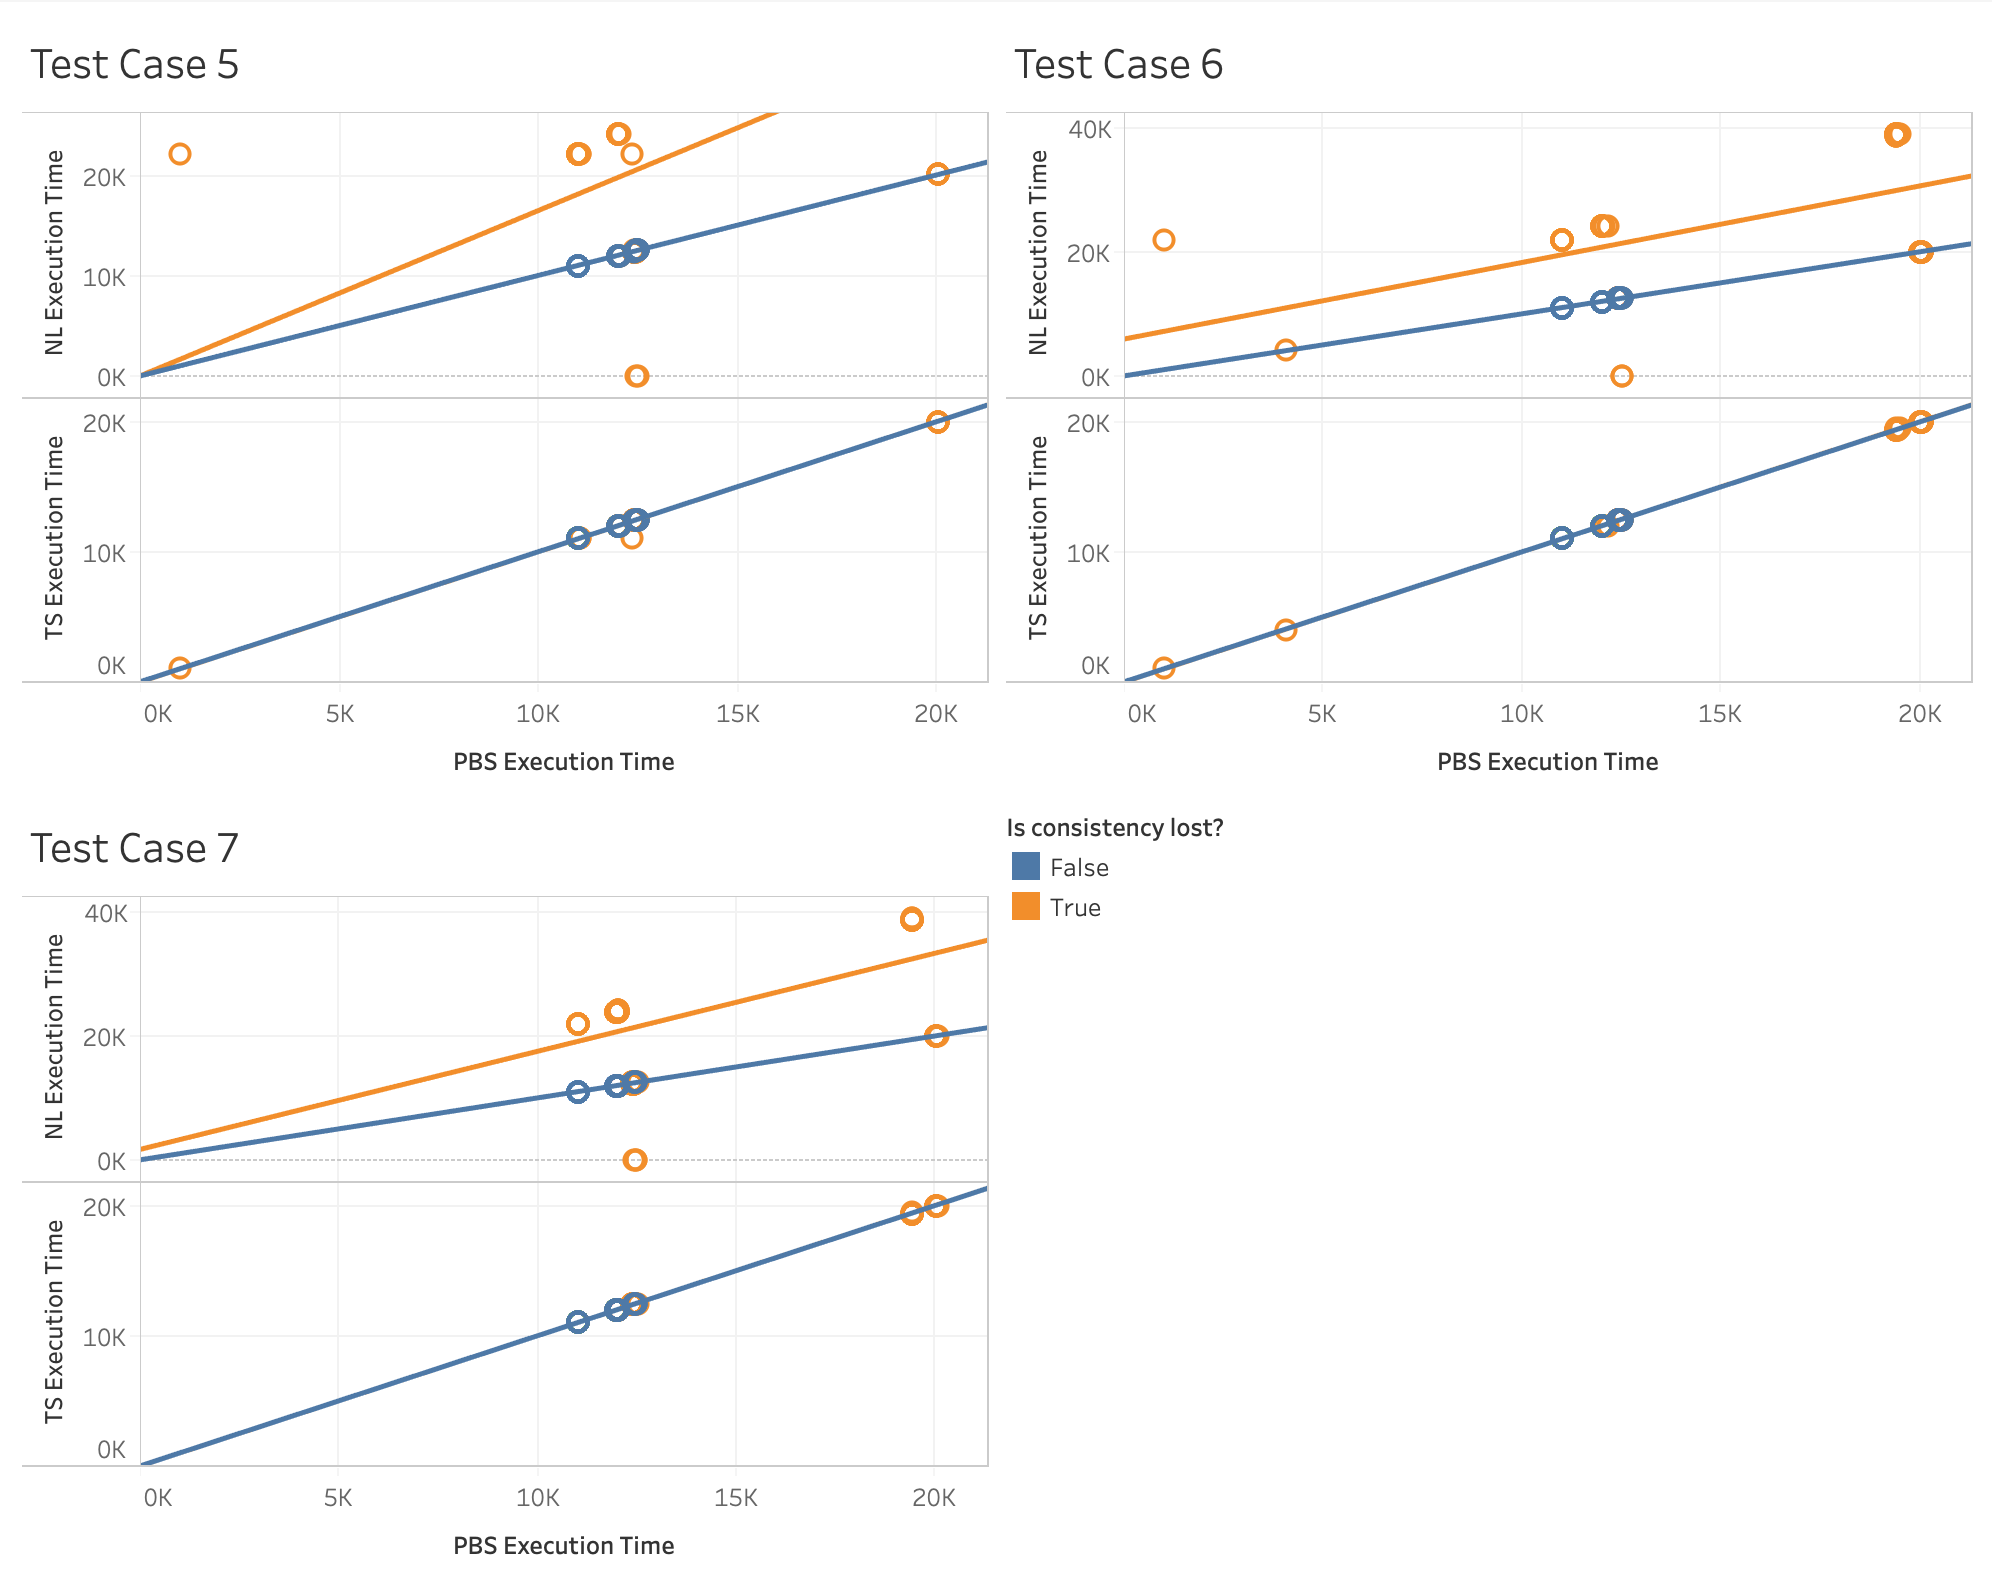
\includegraphics[scale=0.40]{images/Dashboard2_TL.png}
\caption{Consistency Lost/Kept for Test Cases 5-7}
\label{results:consistency_test_case_graphs_5_7}
\end{figure}

\section{Conclusion}
\label{pbs:conclusion}
In summary, transactions within a web service context have always been given a higher priority to efficiency over consistency, and for good reason. When web services are collaborated together by business process languages, the time it takes to complete can be a duration of hours and performance cannot be sacrificed. However, allowing the underlying database to reach an inconsistent state frequently is not acceptable. With the prediction-based solution, we ensure consistency without the performance hit of traditional locking. The three scheduler actions (\textit{grant, decline,} and \textit{elevate}) combined with the four transactional categories ($HCHE$, $HCLE$, $LCHE$, and $LCLE$) develop a solution that can easily be extended to a distributed web service context, in order to improve the current concurrency control mechanisms available today. Our ongoing work aims to prevent malicious transactions from corrupting databases in a web service environment. Liu and Jajodia proposed a multi-phase confinement system that provided a certain level of intrusion tolerance for database systems \cite{Liu_Intrusion}. We believe their model can be expanded using the metrics similar to the ones presented here.

\subsection{Concluding Remarks}
Now that we have established a foundation for prediction-based schedulers, we can now focus on the reputation of the transactions themselves. In the next chapter, this is where we will place our focus. Chapter \ref{chap:prediction_based_scheduler} presented the solution and operated under the assumption that the reputation of the transactions were already established. Chapter \ref{chap:dynamic_reputation} focuses on exactly how the transactions establish their reputation and also dynamically increase or decrease their reputation.

% Transactional correctness and consistency in web service based database transactions are still an after-thought. With the compensation transactions solution, having transactions generate inconsistent states has become acceptable. We show that the prediction-based performance metric that is proposed here is a scalable and efficient solution to web service transactions. This would drastically minimize the amount of compensation transactions needed to ensure consistency in concurrent database transactions. We also show that the solution will ensure a consistent state for transactions that have built a reputation for being reliable under the calculated performance metric. %% Chapter 2
\chapter{Dynamic Transactional Reputation }
\label{chap:dynamic_reputation}

\section{Overview}
\label{drp:overview}
In this chapter, we present the dynamic reputation management system. The work contributed here extends the existing prediction-based scheduler presented in Chapter \ref{chap:prediction_based_scheduler}. The work here in Chapter \ref{chap:dynamic_reputation} is submitted to ACM Transactions on Information Systems and awaiting review.

\section{Introduction}
\label{sec:introduction}

Concurrency control is a problem that has always been at the forefront of researchers for some time now. In traditional database systems, the schedulers provide \gls{acid} properties to transactions that are executed to ensure consistency and correctness. While this is the ideal solution for all transaction scheduling, it's not feasible when transactions are moved to a web service context. The overhead of the locking within web service transactions eliminates the use of traditional scheduling techniques. In order to increase efficiency of many concurrent transactions, the transactional properties of atomicity and isolation are relaxed to prevent the overhead of locking. While this increases efficiency of concurrent transactions, this places the database at a much higher risk of reaching an inconsistent state where data needs to be repaired. The current industry standard is to abandon locking and generate compensating transactions to fix the effects when consistency is lost however, compensating transactions can be very expensive when multiple conflicts occur. In previous work (\cite{ravan_ensuring_2020}) we developed a transaction scheduler that provided a prediction-based analytic to the transaction executing. We used transaction metrics from previous executions to place the transaction in a hierarchical category where we then provided targeted locking. For those transactions that were considered well-behaving, we allow concurrent executions with no locking but those that could potentially cause a cascading rollback, we provided locking to ensure that no other transactions were affected. Going forward in this work we'll simply refer to the prediction-based scheduler as PBS for brevity. 

In this work, we build upon the \gls{pbs} by focusing on the reputation management of the transactions. We use bit-wise scoring based on commit ranking (see Definition \ref{def:commit_ranking}),  efficiency ranking (see Definition \ref{def:efficiency_ranking}), user ranking (see Definition \ref{def:user_ranking}), and system ranking (see Definition \ref{def:system_abort_ranking}) of transactions entering the system. The bit-wise score is then used in a linear fashion to determine locking behaviors for those transactions. Higher scores receive precedence over lower scores therefore allowing for a more granular scheduler that was previously restricted to four categories (see \cite{ravan_ensuring_2020}).

% We focus on identifying classes of transactions (see Definition \ref{transaction_class}) based on the attributes of the transactions and then build a reputation score for those transaction classes. First, we separate the intrinsic (see Definition \ref{intrinsic_attributes}) and extrinsic (see Definition \ref{extrinsic_attributes}) attributes of transactions. The intrinsic attributes are used to identify a particular class of similar transactions. The extrinsic attributes are then used to create a score for the transaction class. 

The scores are calculated after each execution so that the most recent execution's metrics can be taken into consideration. This also prevents adding overhead to the transaction scheduler when transactions enter the system. The score will have already been calculated and a scheduling decision can be made at execution time. The following work details the reputation management system. This chapter is organized in the following order; Section \ref{sec:problem_definition} outlines the problem along with a use-case scenario. Section \ref{sec:related_work} discusses the existing research that has already taken place in regards to the problem. Section \ref{sec:system_model} outlines the system model for the solution. Section \ref{sec:empirical_results} illustrates the simulation results gathered from the prototype.


\section{Problem Definition}
\label{sec:problem_definition}

In order to define the problem of stale transaction categories we must first discuss the problem of concurrent database transactions in a web service environment.

In traditional database systems, transactions are executed with \gls{acid} properties to ensure correctness, durability, and consistency among all transactions that are executed on the system. When transactions are moved to a web service context where concurrent transactions occur frequently, the traditional model of transaction correctness is not feasible to deploy. Multiple interleaving transactions with the locking required in \gls{acid} systems causes an overhead that is not acceptable for the end user. In order to accommodate concurrent transactions in a web service environment that execute in an acceptable time frame, locking is removed and transactions are allowed to execute and commit independently. While all transactions are executing and committing successfully then there are no solutions and the lack of locks works. However, in the event that a transaction fails and there are transactions that are dependent downstream then a cascading rollback occurs reverting the effects of the downstream transaction. All transactions are put on hold until a compensation transaction, generated by the scheduler to fix the results of the failed transaction, can execute successfully. This causes a lot of overhead in the system that can be avoided if the failed transaction can be isolated from dependent transactions.

In our previous work (see \cite{ravan_ensuring_2020}) we presented a prediction-based transaction scheduler that provides appropriate run times for web service environments. The scheduler predicts the outcome of a transaction based on the transactions execution history. The transaction is then placed into one of four categories based on whether commit rate and execution time. We then provided custom locking actions based on the transactional category. Transactions in categories with high commit rates and low execution times are allowed to execute concurrently while transactions in categories with low commit rates and long execution times are locked to prevent downstream effects.

Our previous work addresses the problem of cascading rollbacks and compensation transactions, however a new problem presents itself in a transaction that has been incorrectly categorized or its metrics have changed and it needs to be re-categorized. This becomes a problem when a transaction with a high commit rate is locked due to its category when it can execute concurrently without any undesired side effects. The other extreme and more disastrous use case is a transaction with a low commit rate that should be locked but executes concurrently with other transactions and causes those transactions to abort their executions. In these situations we need the ability to promote or demote a transaction as its execution history changes. 

As we discuss the use of the transaction's execution history, another problem presents itself; what do we do with transactions that are new to the system and do not have any execution history? If we are to address the problem of transactions with no execution history then a reputation score should take the place of the previous four category solution. An objective reputation score allows for a linear approach for transaction comparisons that provides two benefits; a more granular comparison (i.e. comparing transactions that would normally be within the same category and would previously conflict) and a default score for a transaction with no history. In the previous four category solution, there is no default category for transactions with no history. 

In our previous solution, we defined three different locking actions; grant (+), decline (-), and elevate ($\delta$). The decline action causes a transaction to wait for resources to become available. Due to the restrictive four categories of our previous solution, there are a large number of scenarios where a decline action would occur. By transitioning to a solution that is more granular, we could potentially turn decline actions into elevate actions. The elevate action will abort a transaction of a lower category in order for a transaction of a higher category to be granted access to needed resources. By design this prevents transactions that are well-behaving from being hindered by transactions that are not well-behaving. However, if we don't include the cost of an aborted transaction in our calculation then we could do more harm than good by elevating too frequently. Transitioning to a new metric will allow us too refine our rules for elevation to prevent elevate actions that cause more harm than benefit. See Tables \ref{tbl:read_lock_compatibility} and \ref{tbl:write_lock_compatibility} for reference. In the next section we walk through an airline ticketing use-case scenario to better explain the problems identified.

% This situation assumes that not only can the transaction be categorized but it can also be identified from other transactions executing in the system. Transaction identification will allow for a transaction to be identified from other transactions in the system and provide a uniqueness that can be pinpointed. This also shows that the transaction's execution should be translated into an objective reputation metric that can be scored as the execution history grows. 

\subsection{Use-Case Scenario}
\label{subsec:use_case_scenario}

In order to better explain the problems, let's look at a use case scenario of an airline ticketing system. Let's say we have two users that are attempting to reserve seats on an airline. The first user places a ticket, or a seat, in their shopping cart using an airline's online reservation system. While in the shopping cart, that seat is no longer available for reservation even though the transaction has not been completed. Simultaneously, a second user attempts to reserve a seat on the same airline and same flight. There are no seats available so that user is denied a reservation. Later on, the first user that placed the initial reservation in their shopping cart does not purchase the reservation in time. Their reservation is then expired and made available again.

In this scenario, the seat is made available due to the reconciliation efforts of the reservation system, however, in the end the airline loses profit. A seat that could have been purchased by the second user was not available due to the first user having placed the seat in their shopping cart. See the scenario diagram in Figure \ref{image:airline_reservation}. Figure \ref{image:airline_reservation_system_model} shows the same scenario with the transaction scheduler and database contained within the same logical unit. In both figures the solid lines represent the user transactions submitted to the database while the dotted lines represent the response from the transaction. The gray swim lanes labeled $T_0$, $T_1$, and $T_2$ show the transactions at certain time intervals.

\begin{figure}
\centering
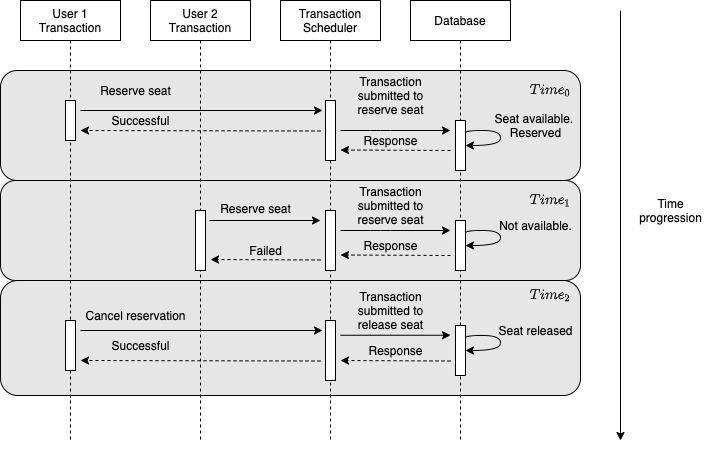
\includegraphics[scale=0.50]{images/AirlineReservation.png}
\caption{Airline Reservation Use Case}
\label{image:airline_reservation}
\end{figure}

\begin{figure}
\centering
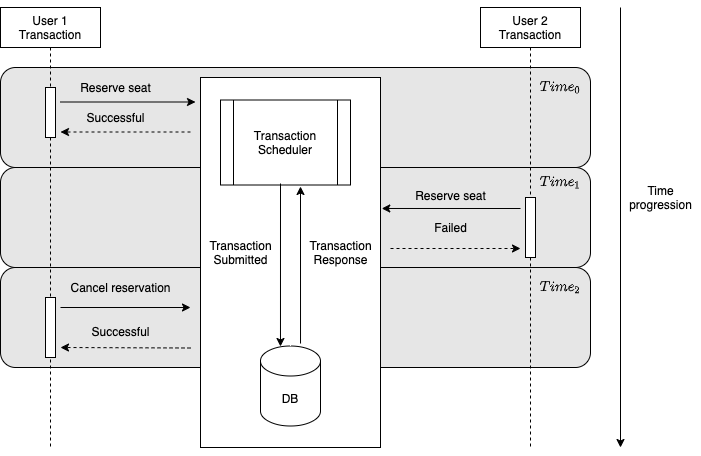
\includegraphics[scale=0.50]{images/AirlineReservation_Overview.png}
\caption{Airline Reservation Use Case System Model}
\label{image:airline_reservation_system_model}
\end{figure}

If the given scenario were to play out in a system that maintained the reputation of transactions entering the system, then the behavior of the first user would be tracked would be taken into consideration. The next time the user were to submit a similar transaction, that reputation would be taken into consideration and could potentially prevent the user from getting precedence over the seat reservation. This reinforces good user behavior in the system and also increases profit for the reservation system. In the next section, we discuss the related work that influenced the current problem and research.
\section{Related Work}
\label{sec:related_work}

There are many resources available for dynamic reputation management that shaped our understanding of the challenges of maintaining reputation of nodes/services. Many of the reputation systems were centered around maintaining a reputation in a distributed or decentralized system. These resources were \cite{clark_dynamic_2017}, \cite{de_paola_reputation_2008}, and  \cite{hu_reputation_2010}. While this helped our understand of the challenges of reputation management, our system would not experience the challenges associated with a decentralized trust management solution since the service and the database are both contained within the prediction-based scheduler itself. Other reputation management solutions were focused on the reputation or trustworthiness of web pages. Those solutions were presented in \cite{melnikov_towards_2018}, \cite{wang_research_2008}, and \cite{zhang_how_2012}. These were also helpful but didn't address the reputation of database transactions directly which is the focus of the reputation of the prediction-based solution. The majority of reputation management systems are provided with the context of P2P or ad-hoc mobile networking in mind. Resources focused on dynamic reputations within networking environments are \cite{chiejina_dynamic_2014}, \cite{de_paola_reputation_2008}, \cite{hu_reputation_2010}, and  \cite{sun_dynamic_2019}.

We also looked at various multi-agent reputation systems to understand how their reputation management systems were leveraged. Reputation management within multi-agent systems, web service selection, and e-commerce has been researched more in depth than reputation within database systems. This gave us a different perspective into reputation management that we could transfer to our database solution. The solutions we reviewed were "Multiagent reputation management to achieve robust software using redundancy" by Rajesh Turlapati (see \cite{rajesh_turlapati_multiagent_2005}), "Multiagent System for Reputation–based Web Services Selection" by Wang et. al. (see \cite{wang_multiagent_2006}), and "Swarm Intelligence Based Reputation Model for Open Multi Agent Systems" by Mahmood et. al. (see \cite{mahmood_swarm_2006}).

Understanding how the user plays a role with the outcome of the transaction is a key piece of our solution. Looking at the work presented by Lomet et. al. (\cite{lomet2006recovery}) motivated our inclusion of the User Ranking (see Definition \ref{def:user_ranking}) in our solution.

To better understand data lineage and how it can be used as a tool for building transactional reputations we looked at our previous research of data provenance and malicious transactions in Theppatorn et. al. (\cite{theppatorn_2021}).

A great deal of the existing work related to concurrency control (e.g., \cite{Alrifai_Distributed_Managment}, \cite{Fekete_RAMP}, \cite{dai_qos-driven_2009}, \cite{WSCO}, \cite{ferreira_transactional_2012}, \cite{WSBA}, \cite{zhengdong_gao_combining_2005}, \cite{Fekete_IsolationSupport}, \cite{Fekete_Promises}, \cite{Eunhee_PredictionBasedCC}, \cite{kang-woo_lee_consistency_2000}, \cite{WSAT}, \cite{olmsted_long_2015}, and \cite{Riegen_RuleBased}) influenced our motivation for this work.

After studying the current environment of dynamic reputation systems, we believe this is a great opportunity to provide a dynamic reputation management solution particularly focused at database transactions within a web service environment.
\section{System Model}
\label{sec:system_model}
This section covers the system model. Here we discuss the definitions, implementation, and environment involved in the dynamic reputation solution.

\subsection{Definitions}
\label{rep:definitions}

There are multiple definitions within Chapters \ref{chap:prediction_based_scheduler} \& \ref{chap:multi_level_security} that will be used as a part of the VRM extension. There will also be changes to existing definitions and new definitions to properly implement and define the VRM solution.
% \subsection{Transaction Identification}
\label{sec:transaction_identification}
The first problem of properly maintaining a transactional reputation is establishing the ability to identify a class of transactions. We must identify a class of transactions otherwise every unique transaction will be given its own reputation. For example, in Figure \ref{fig:transaction_classes} we see that $T_{1}$ and $T_{2}$ have the same number of operations, the same order of operations, and executed by the same user. The only difference between the two transactions is the that the resources is differ. $T_{1}$ and $T_{2}$ are good candidates for its own transaction class that contain the same reputation diagnosis rather than operating as separate reputations. On the other hand, $T_{3}$ and $T_{4}$ would not be candidates for a transaction class. While they are executed by the same user, they do not have the same number of matching operations.


\begin{figure}[h]
\captionsetup{justification=centering}
\centering % used for centering Figure

\begin{picture}(50,50)
    \put(-75,50){$T_{1}{user_{1}}$ = $R_{1}(a)R_{2}(b)R_{1}(b)W_{2}(b)R_{2}(a)W_{2}(a)$}
     \put(-75,35){$T_{2}{user_{1}}$ = $R_{1}(c)R_{2}(a)R_{1}(a)W_{2}(d)R_{2}(b)W_{2}(c)$}
     \put(-75,20){$T_{3}{user_{2}}$ = $R_{1}(a)R_{2}(b)R_{1}(b)W_{2}(b)R_{2}(a)W_{2}(a)$}
     \put(-75,5){$T_{4}{user_{2}}$ = $R_{1}(c)R_{2}(a)R_{1}(a)W_{2}(d)$}
\end{picture}

\caption{Transaction Classes} % title of the Figure
\label{fig:transaction_classes} % label to refer figure in text

\end{figure}

In order to create transaction classes we must separate intrinsic and extrinsic attributes of a transaction. This pattern of separating the unique attributes (see Definition \ref{intrinsic_attributes}) from the common attributes (see Definition \ref{extrinsic_attributes}) is known as the Flyweight Design Pattern in Software Engineering (see \cite{gof:1994}).

The Flyweight Software Design Pattern was originally developed to save space for in-memory applications by sharing a common objects rather that creating new objects each time. While we're not concerned about memory usage in this application, the Flyweight pattern provides a framework for separating the common attributes (intrinsic state) from the specific attributes (extrinsic state). Once we have these separated we can use the intrinsic state to define a transaction class (see Definition \ref{transaction_class}) while using the extrinsic attributes to calculate a reputation score.

Table \ref{tbl:intrinsic_and_extrinsic_attributes} shows transactional attributes that are used in the identification of a transaction class (intrinsic) and the attributes that are used in identifying the reputation of a transaction class (see Definition \ref{transaction_class}).

\begin{table}[h]
\caption{Intrinsic \& Extrinsic Transactional Attributes}
\captionsetup{justification=centering}
\centering
\begin{tabular}{|c|c|c|}
\hline
\multicolumn{2}{|c|}{\cellcolor[HTML]{EFEFEF}\textbf{Transaction Class Attributes}}                                                   \\ \hline
\textbf{Intrinsic} & \textbf{Extrinsic}   \\ \hline
\# of Operations  &  Execution Time         \\ \hline
Order of Operations  &  Commit Rate      \\ \hline
User             & Resources            \\ \hline
\end{tabular}
\label{tbl:intrinsic_and_extrinsic_attributes}

\end{table}
\subsection{Reputation Score}
\label{sec:reputation_score}

In order to construct the reputation of a transaction we construct a 4-tuple score (see Definition \ref{def:reputation_score}) based on the four transactional attributes of commit ranking (see Definition \ref{def:commit_ranking}), efficiency ranking (see Definition \ref{def:efficiency_ranking}), user ranking (see Definition \ref{def:user_ranking}), and system ranking (see Definition \ref{def:system_abort_ranking}). Each of the four values associated with the reputation score is a normalized value between 0 and 1 that ranks the transaction among all transactions executing within the system. Each value also contains a weighted multiplier that can be used in order to reward or place a higher precedence on a particular attribute for a particular transaction. If the multiplier is equal to one then all attributes contribute to the score equally.

Previously, the solution only kept commit rate and efficiency rate into consideration when categorizing transactions. This created a four category system that wouldn't allow dominance of transactions within the same category. By using the reputation score, we can now establish dominance of transactions that would originally have been in the same category. The next section discusses this dominance structure.

% In order to construct the reputation of a transaction class we use a bit-wise scoring system based on the four transactional attributes of commit ranking (see Definition \ref{def:commit_ranking}), efficiency ranking (see Definition \ref{def:efficiency_ranking}), user ranking (see Definition \ref{def:user_ranking}), and system ranking (see Definition \ref{def:system_abort_ranking}). The bit-wise score consists of using one byte for each attribute that can then be used to make more granular locking decisions. Our previous system of transactional categories (see Figure \ref{graph:cat_graph}) only allows for four possibilities of decision making. By moving to a bit-wise scoring system, we can then have a linear system of promoting and demoting transactions. This allows for a more granular approach that breaks down the walls of a strict four category system and allows for promotion and demotion of transactions that would normally be contained within the same category. With one byte representing each attribute (see Figure \ref{image:bitwise_reputation_score}), we then have 1,024 possible combinations that provide a much granular system than the previous four categories.

% The bit-wise score for each transaction will have one byte allocated for each transactional attribute for a total of thirty-two bits. From there we use positive reinforcement in order to increment or decrement the score. The scoring rules are shown below in Table \ref{tbl:scoring_matrix}.

% As you can see from the rules shown in Table \ref{tbl:scoring_matrix} we don't increment the individual scores unless they are within upper and lower twenty percentile. This prevents changing the score on every execution and allows the system to adjust gradually.


% \begin{table}[h]
% \captionsetup{justification=centering}
% \centering
% \begin{tabular}{|c|c|c|}
% \hline
% \multicolumn{2}{|c|}{\cellcolor[HTML]{EFEFEF}\textbf{Bit-Wise Scoring Values}}                                                   \\ \hline
% \textbf{Attribute Value} & \textbf{Scoring Value}   \\ \hline
% Commit Rate $<$ 20\%            &  -1        \\ \hline
% Commit Rate $>$ 80\%            &  +1        \\ \hline
% Efficiency Rate $<$ 20\%        &  +1        \\ \hline
% Efficiency Rate $>$ 80\%        &  -1        \\ \hline
% User Reputation $<$ 20\%        &  +1        \\ \hline
% User Reputation $>$ 80\%        &  -1        \\ \hline
% Forced Abort                    &  +2        \\ \hline
% Success after Forced Abort      &  -2        \\ \hline
% \end{tabular}

% \caption{Bit-Wise Scoring Matrix}
% \label{tbl:scoring_matrix} 

% \end{table}

% \begin{figure}
% \centering
% 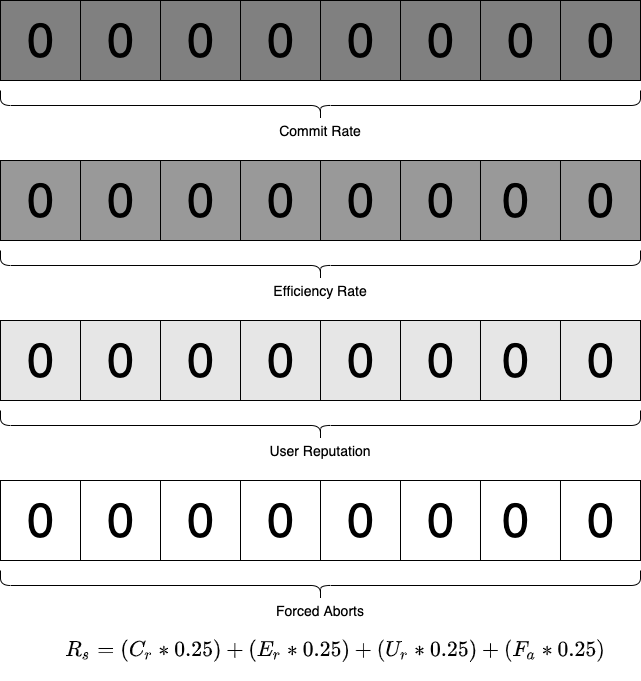
\includegraphics[scale=0.30]{images/BitwiseScore.png}
% \caption{Bit-Wise Reputation Score}
% \label{image:bitwise_reputation_score}
% \end{figure}
\subsection{Strong \& Weak Dominance}
\label{sec:dominance}

In our previous work of \gls{pbs} we presented the transaction dominance lattice (see Figure \ref{fig:category_lattice_2}) that establishes dominance of transactions that were categorized. While the prediction-based solution adds categorization to provide a solution against conflicting transactions, there is still the limitation that two transactions of the same categorization can be in conflict. In this situation, the prediction-based solution reverts to existing 2PL with no added benefit.

% \createCategorizationGraph{graph:cat_graph}{Categorization Graph}

\[\textrm{$HCHE > HCLE > LCLE$}\]
\[\textrm{$HCHE > LCHE > LCLE$} \]

\begin{figure}[h]
\captionsetup{justification=centering}
\centering % used for centering Figure

\begin{tikzpicture}
    % [list/.style={rectangle split, rectangle split parts=3,
    % draw, rectangle split horizontal}, >=stealth, start chain]
  \node[text width=1.5cm] at (4.4,5) {$HCHE$};
  \node[text width=1.5cm] at (3.4,4) {$HCLE$};
  \node[text width=1.5cm] at (5.4,4) {$LCHE$};
  \node[text width=1.5cm] at (4.4,3) {$LCLE$};
  \draw (4.0,4.8) -- (3.2,4.2);
  \draw (4.1,4.8) -- (4.9,4.2);
  \draw (4.0,3.2) -- (3.2,3.8);
  \draw (4.1,3.2) -- (4.9,3.8);
  
\end{tikzpicture}

\caption{Transaction Category Dominance} % title of the Figure
\label{fig:category_lattice_2} % label to refer figure in text

\end{figure}

By transitioning to a solution that contains a continuous spectrum of categorization, we can avoid the situation where two transactions of the same categorization cause a conflict. Tables \ref{tbl:read_lock_compatibility} \& \ref{tbl:write_lock_compatibility} show the existing rules for the four category solution. The existing operations would apply given the rules of dominance (see Definitions \ref{def:strong_dominance}, \ref{def:weak_dominance}, and \ref{def:not_comparable}) to execute and eliminate situations in which transactions of the same category would normally conflict.

Strong Dominance (see Definition \ref{def:strong_dominance}) is established when all four attributes of a reputation score of a transaction (commit ranking, efficiency ranking, user ranking, and system ranking) contain a value that is greater than all the values of the conflicting transactions reputation score. This the most preferred and easiest way to establish dominance between two conflicting transactions.

If Strong Dominance cannot be established then there is the ability to still obtain a "tie breaking" situation with Weak Dominance (see Definition \ref{def:weak_dominance}). Weak Dominance can be established by taking a sum of all four attributes of each transaction's reputation score and doing a numerical comparison of the overall score. If the score of the conflicting transaction is greater than or equal to the other transaction, then Weak Dominance is established preventing a stalemate.

If neither Strong or Weak Dominance can be established then we have reach a state of Not Comparable (see Definition \ref{def:not_comparable}). If the two conflicting transactions are deemed Not Comparable then the precedence of the two transactions will take priority and the conflicting transaction mus wait for the first transaction to complete.


% Figure \ref{image:vrm} displays a visual of the VRM solution where there are upper and lower bounds for reputation scores. This prevents transactional classes from being penalized or awarded to such an extent that they either cause starvation of other transactions or they suffer from starvation themselves. The plots along the vector represent the reputation scores of particular transactions. This figure gives a visual representation of the precedence of the transactions. Since the vector is not broken into four categories (see Figure \ref{graph:cat_graph} for a reference to our previous solution) there is a much granular and precise decision of which transaction takes precedence. With the VRM solution we no longer have to revert to 2PL for two transactions within the same category because we now have a numerical score that we can use for locking decisions.

% \begin{figure}
% \centering
% 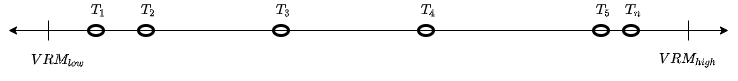
\includegraphics[scale=0.30]{images/VRM.png}
% \caption{Vector Reputation Management}
% \label{image:vrm}
% \end{figure}

% \begin{table}[h]
% \captionsetup{justification=centering}
% \centering
% \begin{tabular}{l|c|c|c|c|c|c|}

% \cline{2-5} & 
% \multicolumn{4}{c|}{\textbf{already granted lock}} \\

% \cline{2-5} \hline

% \multicolumn{1}{|l|}{\begin{tabular}[c]{@{}c@{}}\textbf{requested}\\\textbf{lock}\end{tabular}} &\textbf{$HCHE_{r}$}    & \textbf{$HCLE_{r}$}    & \textbf{$LCHE_{r}$}     & \textbf{$LCLE_{r}$}    \\ \hhline{=#====}
% \multicolumn{1}{|l||}{\textbf{$HCHE_{r}$}} &\textbf{+}    & \textbf{+}    & \textbf{+}     & \textbf{+}    \\ \hline
% \multicolumn{1}{|l||}{\textbf{$HCLE_{r}$}} &\textbf{+}    & \textbf{+}    & \textbf{+}     & \textbf{+}    \\ \hline
% \multicolumn{1}{|l||}{\textbf{$LCHE_{r}$}} &\textbf{+}    & \textbf{+}    & \textbf{+}     & \textbf{+}    \\ \hline
% \multicolumn{1}{|l||}{\textbf{$LCLE_{r}$}} &\textbf{+}    & \textbf{+}    & \textbf{+}     & \textbf{+}    \\ \hline
% \multicolumn{1}{|l||}{\textbf{$HCHE_{w}$}} &\textbf{-}    & $\delta$      & $\delta$       & $\delta$        \\ \hline
% \multicolumn{1}{|l||}{\textbf{$HCLE_{w}$}} &\textbf{-}    & \textbf{-}    & $\delta$       & $\delta$        \\ \hline
% \multicolumn{1}{|l||}{\textbf{$LCHE_{w}$}} &\textbf{-}    & \textbf{-}    & \textbf{-}     & $\delta$        \\ \hline
% \multicolumn{1}{|l||}{\textbf{$LCLE_{w}$}} &\textbf{-}    & \textbf{-}    & \textbf{-}     & \textbf{-}    \\ \hline           
% \end{tabular}

% \caption{Read-Lock Compatibility} % title of the Figure
% \label{tbl:read_lock_compatibility} % label to refer figure in text

% \end{table}


% \begin{table}[h]
% \captionsetup{justification=centering}
% \centering
% \begin{tabular}{l|c|c|c|c|c|c|}

% \cline{2-5} & 
% \multicolumn{4}{c|}{\textbf{already granted lock}} \\

% \cline{2-5} \hline

% \multicolumn{1}{|l|}{\begin{tabular}[c]{@{}c@{}}\textbf{requested}\\\textbf{lock}\end{tabular}} &\textbf{$HCHE_{w}$}    & \textbf{$HCLE_{w}$}    & \textbf{$LCHE_{w}$}     & \textbf{$LCLE_{w}$}    \\ \hhline{=#====}
% \multicolumn{1}{|l||}{\textbf{$HCHE_{r}$}} &\textbf{-}    & $\delta$    & $\delta$     & $\delta$    \\ \hline
% \multicolumn{1}{|l||}{\textbf{$HCLE_{r}$}} &\textbf{-}    & \textbf{-}    & $\delta$    & $\delta$    \\ \hline
% \multicolumn{1}{|l||}{\textbf{$LCHE_{r}$}} &\textbf{-}    & \textbf{-}    & \textbf{-}     & $\delta$    \\ \hline
% \multicolumn{1}{|l||}{\textbf{$LCLE_{r}$}} &\textbf{-}    & \textbf{-}    & \textbf{-}     & \textbf{-}    \\ \hline
% \multicolumn{1}{|l||}{\textbf{$HCHE_{w}$}} &\textbf{-}    & $\delta$      & $\delta$       & $\delta$        \\ \hline
% \multicolumn{1}{|l||}{\textbf{$HCLE_{w}$}} &\textbf{-}    & \textbf{-}    & $\delta$       & $\delta$        \\ \hline
% \multicolumn{1}{|l||}{\textbf{$LCHE_{w}$}} &\textbf{-}    & \textbf{-}    & \textbf{-}     & $\delta$        \\ \hline
% \multicolumn{1}{|l||}{\textbf{$LCLE_{w}$}} &\textbf{-}    & \textbf{-}    & \textbf{-}     & \textbf{-}    \\ \hline           
% \end{tabular}

% \caption{Write-Lock Compatibility} % title of the Figure
% \label{tbl:write_lock_compatibility} % label to refer figure in text

% \end{table}
\subsection{Locking Actions with Reputation Score}
\label{sec:reputation_score_locking_actions}

Now that we have a system for calculating a reputation score for all transactions that have entered the system, we can use that score and refine our existing locking actions. Tables \ref{tbl:read_lock_compatibility} and \ref{tbl:write_lock_compatibility} show the existing rules for when the three locking actions should be used. These rules were generated when we only had a four-category system. Now that we have reputation score, we need a much more refined formula that defines when to use the elevate action ($\delta$) and the decline action (-).

In the previous model, an elevate or decline action would occur in situations where there was a conflict and the conflicting transactions (see Definition \ref{conflict_ops}) were in different categories. This did not take into account how closely similar or vastly different the two transactions were. It was very black and white could potentially cause extreme overhead due to excessive elevate actions.

In the new model that we present here, we would elevate the transaction that possesses either Strong or Weak Dominance over the conflicting transaction.

Let $T_{1}$ and $T_{2}$ be two conflicting transaction and $A$ = \{$decline (-)$, $elevate (\delta)$\} be the set of locking actions for conflicting transactions. For two conflicting transactions, let the mapping $\tau$ below display actions taken assuming that $T_{1}$ is the transaction with precedence. Therefore:

\[ 
\tau \rightarrow
\left \{
  \begin{tabular}{cc}
  $elevate (\delta)$ & $Dominates_{S}(T_{1},T_{2})$ = false, and \\
   & $Dominates_{W}(T_{1},T_{2})$ = false \\
  $decline (-)$ & $Dominates_{S}(T_{1},T_{2})$ = true \\
  $decline (-)$ & $Dominates_{W}(T_{1},T_{2})$ = true \\
  \end{tabular}
\right \}
\]

This model doesn't apply to grant (+) actions since there is no conflict and no need for conflicting locking action. In the next section we discuss how the reputation score is recalculated and rewards are applied.
\subsection{Reputation Score Recalculation \& Reward}
\label{sec:recalculation_and_reward}

The Reputation Score for a transaction allows us to prioritize transactions based on their transactional attributes. However, we need the ability to recalculate the reputation scores so that the correct actions are being taken. We want to be able to recalculate without the recalculation being a burden on the system with intense overhead.

In order to recalculate the reputation scores in such a way that it does not incur a lot of overhead, we recalculate based on the percentage of transactions that have been aborted. When greater than 10\% of the transactions end execution via an abort within the system, then we recalculate their reputation scores in order to avoid situations that will cause transactions additional overhead or a premature abort.

Recalculating the scores based on this percentage allows the system to make correct decisions regarding locking actions without adding an additional burden to the system. The frequency of score recalculation is then dynamic and changing based on the needs of the system rather than a static time frame. 

% Figure \ref{image:recalculation_graph} gives a visual of the recalculation threshold and how the number of affected transactions will fluctuate within a given system. 

% \begin{figure}
% \centering
% 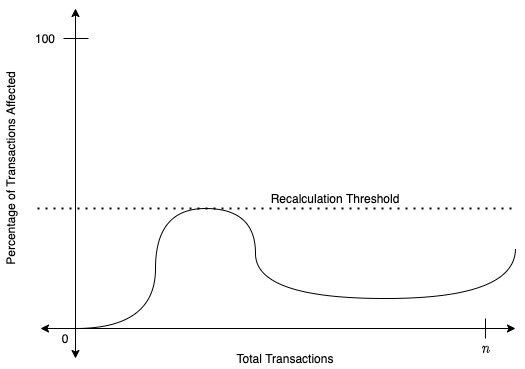
\includegraphics[scale=0.32]{images/RecalculationGraph.png}
% \caption{Graph of Recalculation and Affected Transactions}
% \label{image:recalculation_graph}
% \end{figure}
\subsection{Use Case with Dynamic Reputation Management}
\label{sec:use_case_with_drm}

Now if we take a look at the use case outlined in Section \ref{subsec:use_case} with the Dynamic Reputation Management solution, we can prevent the behavior of user 1 from affecting the other users in the system. Figure \ref{image:airline_reservation_with_drm} shows the use case with the reputation management solution embedded. In this scenario, the bad reputation of user 1 doesn't affect user 2. We have tracked the reputation of user 1 and therefore prevent user 1 from reserving the seat. This then allows the seat to be available for user 2 to reserve and purchase.

\begin{figure}
\centering
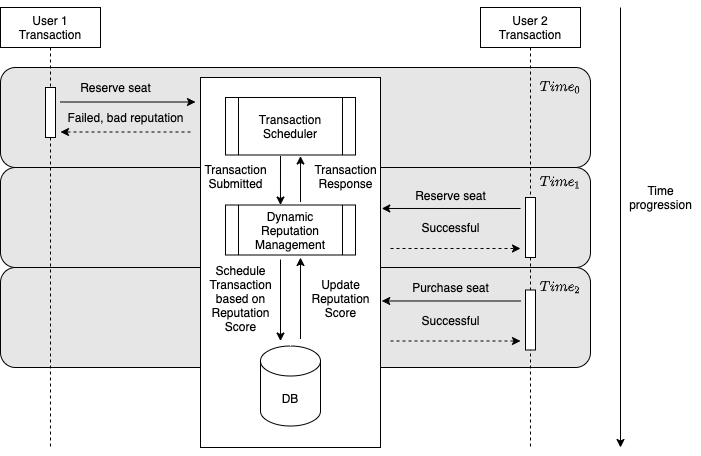
\includegraphics[scale=0.50]{images/AirlineReservation_w_DRM.png}
\caption{Use Case with Dynamic Reputation Management}
\label{image:airline_reservation_with_drm}
\end{figure}
% \subsection{Algorithms}
\label{mls:algorithms}
% \section{Algorithms}
% \label{sec:algorithms}

% This section discusses all the algorithms needed for dynamic reputation management.
\section{Empirical Results}
\label{sec:empirical_results}

Here we discuss the setup and execution of the simulation for dynamic reputations. The prototype is used to generate simulation results and verify results of the executions.

\subsection{Application}
\label{sec:er_application}

In this section, we discuss the application environment used for executing transactions.

The application is written using Spring Boot and Java.
\href{https://spring.io/projects/spring-boot}{Spring Boot} is an application framework that allows Java applications to be containerized easily and manage dependencies within the application itself.

Within the application we have four transaction schedulers implemented

\begin{itemize}
  \item No-Locking Scheduler (NoSQL)
  \item Traditional Scheduler (\gls{2pl})
  \item Prediction-Based Scheduler'
  \item Dynamic Reputation Scheduler
\end{itemize}

Each scheduler is executed with the same execution parameters. Those parameters include

\begin{itemize}
    \item Users
    \item Transactions
    \item Rate of abort
    \item Rate of conflict
    \item Use Case (discussed in next section)
\end{itemize}

Each scheduler executes in its own dedicated thread and we record results for each execution for analysis. Table \ref{tbl:execution_history} is a schema diagram of the results that we capture for each transaction execution.

\begin{table}
\captionsetup{justification=centering}
\centering
 \begin{tabular}{|p{0.28\linewidth} | p{0.5\linewidth}|}
 \hline
 \textbf{Attribute Name} & \textbf{Description} \\ [0.5ex] 
 \hline\hline
%  id & The primary key of the results table \\ 
%  \hline
 userid & Unique identifier for the user  \\
 \hline
 user\_ranking & Decimal value containing user ranking defined in Definition \ref{def:user_ranking}  \\
 \hline
 transactionid & Unique identifier for the transaction \\
 \hline
 commit\_ranking & Decimal value containing user ranking defined in Definition \ref{def:commit_ranking}  \\
 \hline
 system\_ranking & Decimal value containing user ranking defined in Definition \ref{def:system_abort_ranking}  \\
 \hline
 eff\_ranking & Decimal value containing user ranking defined in Definition \ref{def:efficiency_ranking}  \\
 \hline
 num\_of\_operations & Integer value of the number of operations in the transaction  \\
 \hline
 reputation\_score & String representation of all rankings together  \\
 \hline
 transaction\_exec\_time & Decimal representing to the total execution time in milliseconds  \\
 \hline
 percentage\_aborted & Decimal representing to percentage of aborted transactions over the total transactions during that particular execution  \\
 \hline
 recalculation\_needed & Boolean representing if the recalculation threshold was surpassed   \\
 \hline
 time\_executed & Timestamp representing the time of the execution  \\
 \hline
 dominance\_type & String representing what type of dominance was established (see Definitions \ref{def:strong_dominance}, \ref{def:weak_dominance}, and \ref{def:not_comparable})  \\
 \hline
 transaction\_outcome & String representing whether the execution committed, aborted, or aborted due to higher dominance  \\
 \hline
 scheduler\_type & String representing which scheduler submitted the execution  \\
 \hline
 use\_case & String representing what use case this execution was a part of  \\
 \hline
 category & String representing the category of the transaction if it was an execution from PBS  \\
 \hline
 transaction\_type & String representing whether it was as normal or compensation transaction  \\ [1ex] 
 \hline
\end{tabular}
\caption{Execution History Attributes}
\label{tbl:execution_history} % label to refer figure in text
\end{table}

% Once the application is deployed, it is running but the schedulers are not started. In order to start the application, we have to interact with the REST API that is a part of the application.

% \begin{itemize}
%   \item \textbf{/health}
%   \begin{itemize}
%      \item Returns a simple status if the application is running
%   \end{itemize}
%   \item \textbf{/info}
%   \begin{itemize}
%      \item Returns application version to ensure the right version of the application is running
%   \end{itemize}
%   \item \textbf{/start}
%   \begin{itemize}
%      \item This is the endpoint used to start the execution of the schedulers. There is a table that stores the use cases that we wish to run. Once this endpoint is accessed, it will pull the use case that we have configured and begin running with those parameters
%   \end{itemize}
%   \item \textbf{/stop}
%   \begin{itemize}
%      \item This stops the execution of the schedulers
%   \end{itemize}
%   \item \textbf{/update}
%   \begin{itemize}
%      \item This allows us to update the parameters without redeploying the application
%   \end{itemize}
% \end{itemize}

Before we started running the schedulers we generated users and transactions with random rankings between 0 and 1 for an initial working set. We generated over 5800 users and over 11000 transactions.

When the recalculation percentage threshold is reached we recalculate all of the rankings based on our definitions of each ranking (see Section \ref{sec:definitions}). This recalculation takes place in its own thread to prevent blocking the schedulers from continuing with their executions.
\subsection{Use Case Formulation}

We have experimented with a variety of use cases to fine tune our empirical results.  Table \ref{tbl:use_cases_initial} shows the use cases that were executed initially to get a baseline of how transactions within the system would be affected, when a recalculation would occur, and what was the impact of that recalculation. Table \ref{tbl:use_cases} shows our final use case selection for the performance measurement of our approach.
%Before the use cases executed in Table \ref{tbl:use_cases} were developed, there were thousands of transactions executed with a variety of parameters. These initial use cases helped us develop the ideal use cases that would best show the benefits and drawbacks of the new dynamic reputation solution.

For the graphs in this section we use the term \textbf{affected transactions} to identify transactions that were forced to abort by our scheduler.



\begin{table}
\caption{Initial Use Cases}
\captionsetup{justification=centering}
\centering
 \begin{tabular}{|| c | c | c | c | c ||} 
 \hline
 \textbf{Name} & \textbf{Total \#} & \textbf{Recalculation \%} &  \textbf{Conflict \%} & \textbf{Abort \%} \\ [0.5ex] 
 \hline\hline
 Use Case Alpha & $\approx$ 23,000 & 50 & 10 & 5  \\ 
 \hline
 Use Case Beta & $\approx$ 2,500 & 10 & 25 & 25  \\ 
 \hline
 Use Case Gamma & $\approx$ 1,900 & 5 & 40 & 40  \\ 
 \hline
 Use Case Delta & $\approx$ 1,200 & 7 & 50 & 50  \\ 
 [1ex] 
 \hline
\end{tabular}
\label{tbl:use_cases_initial} % label to refer figure in text
\end{table}

Our first preliminary use case (Use Case Alpha shown in Figure \ref{image:use_case_alpha}) started with a high recalculation percentage to get a baseline test of the prototype. The high recalculation percentage (50\%) caused that initially, the affected transactions spiked to approximately 3\%, and then began to level off as the number of transactions within the system increased. We observed that with the 50\% affected transactions rate, recalculation would never be triggered.

\begin{figure}
\centering
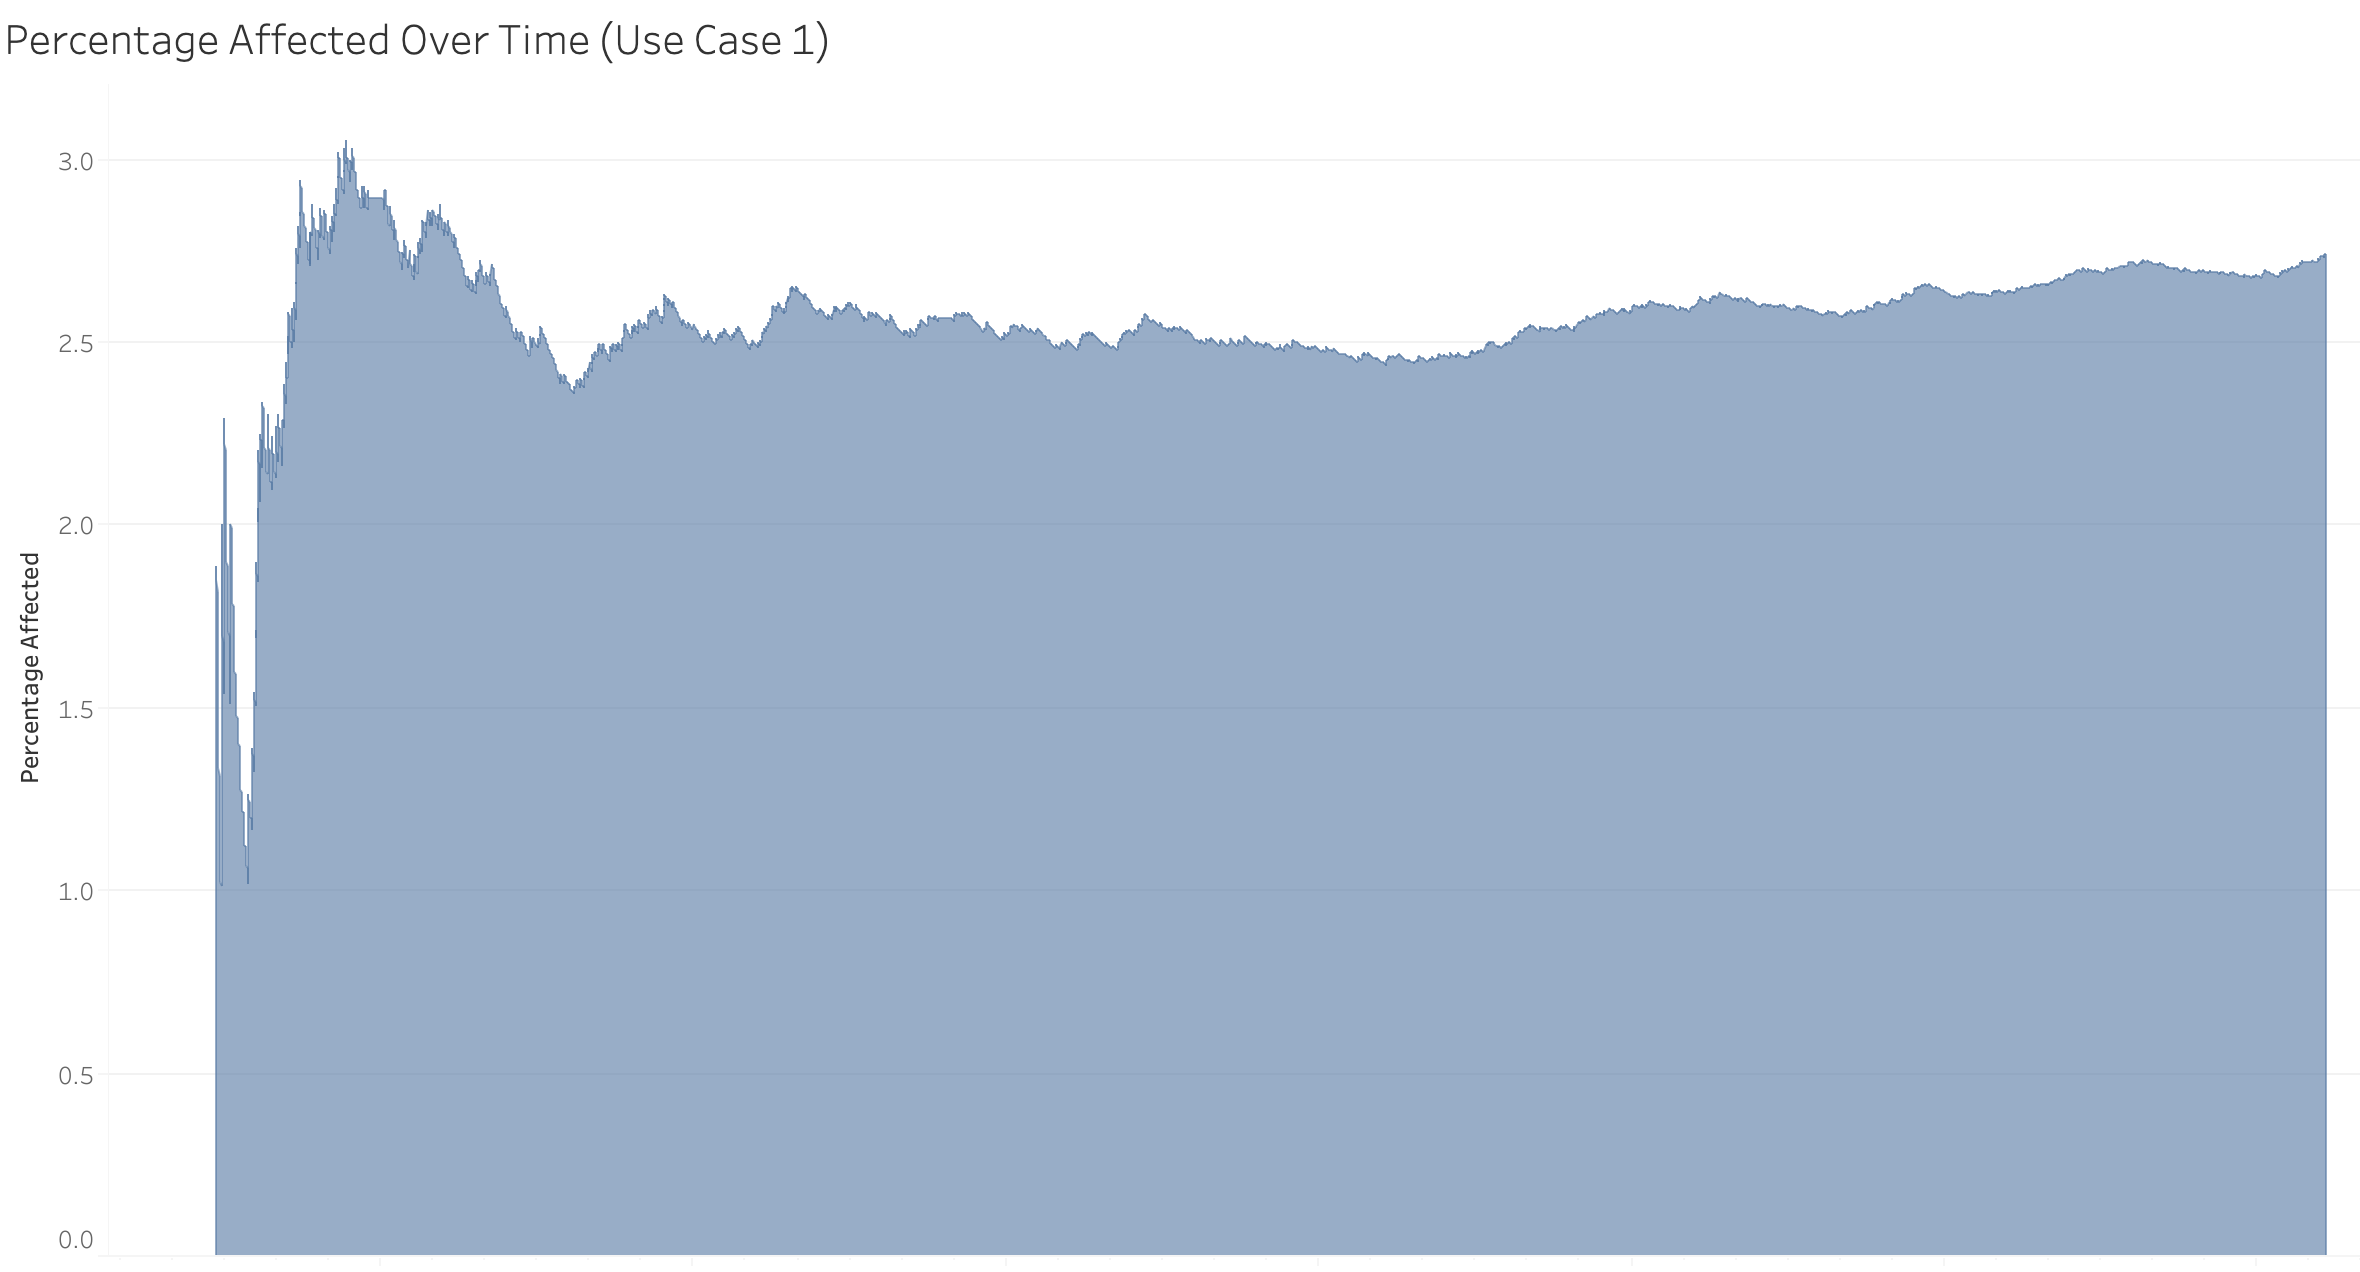
\includegraphics[scale=0.35]{images/UseCase1.png}
\caption{Use Case Alpha}
\label{image:use_case_alpha}
\end{figure}

Our next preliminary use case (Use Case Beta shown in Figure \ref{image:use_case_beta}) decreased the recalculation rate to 10\% while increasing the conflicting and abort percentages in the system to 25\%. This was enough of a change to cause a single recalculation in the beginning. As the number of transactions increased in the system the number of affected transactions would grow too slowly to initiate another recalculation.

\begin{figure}
\centering
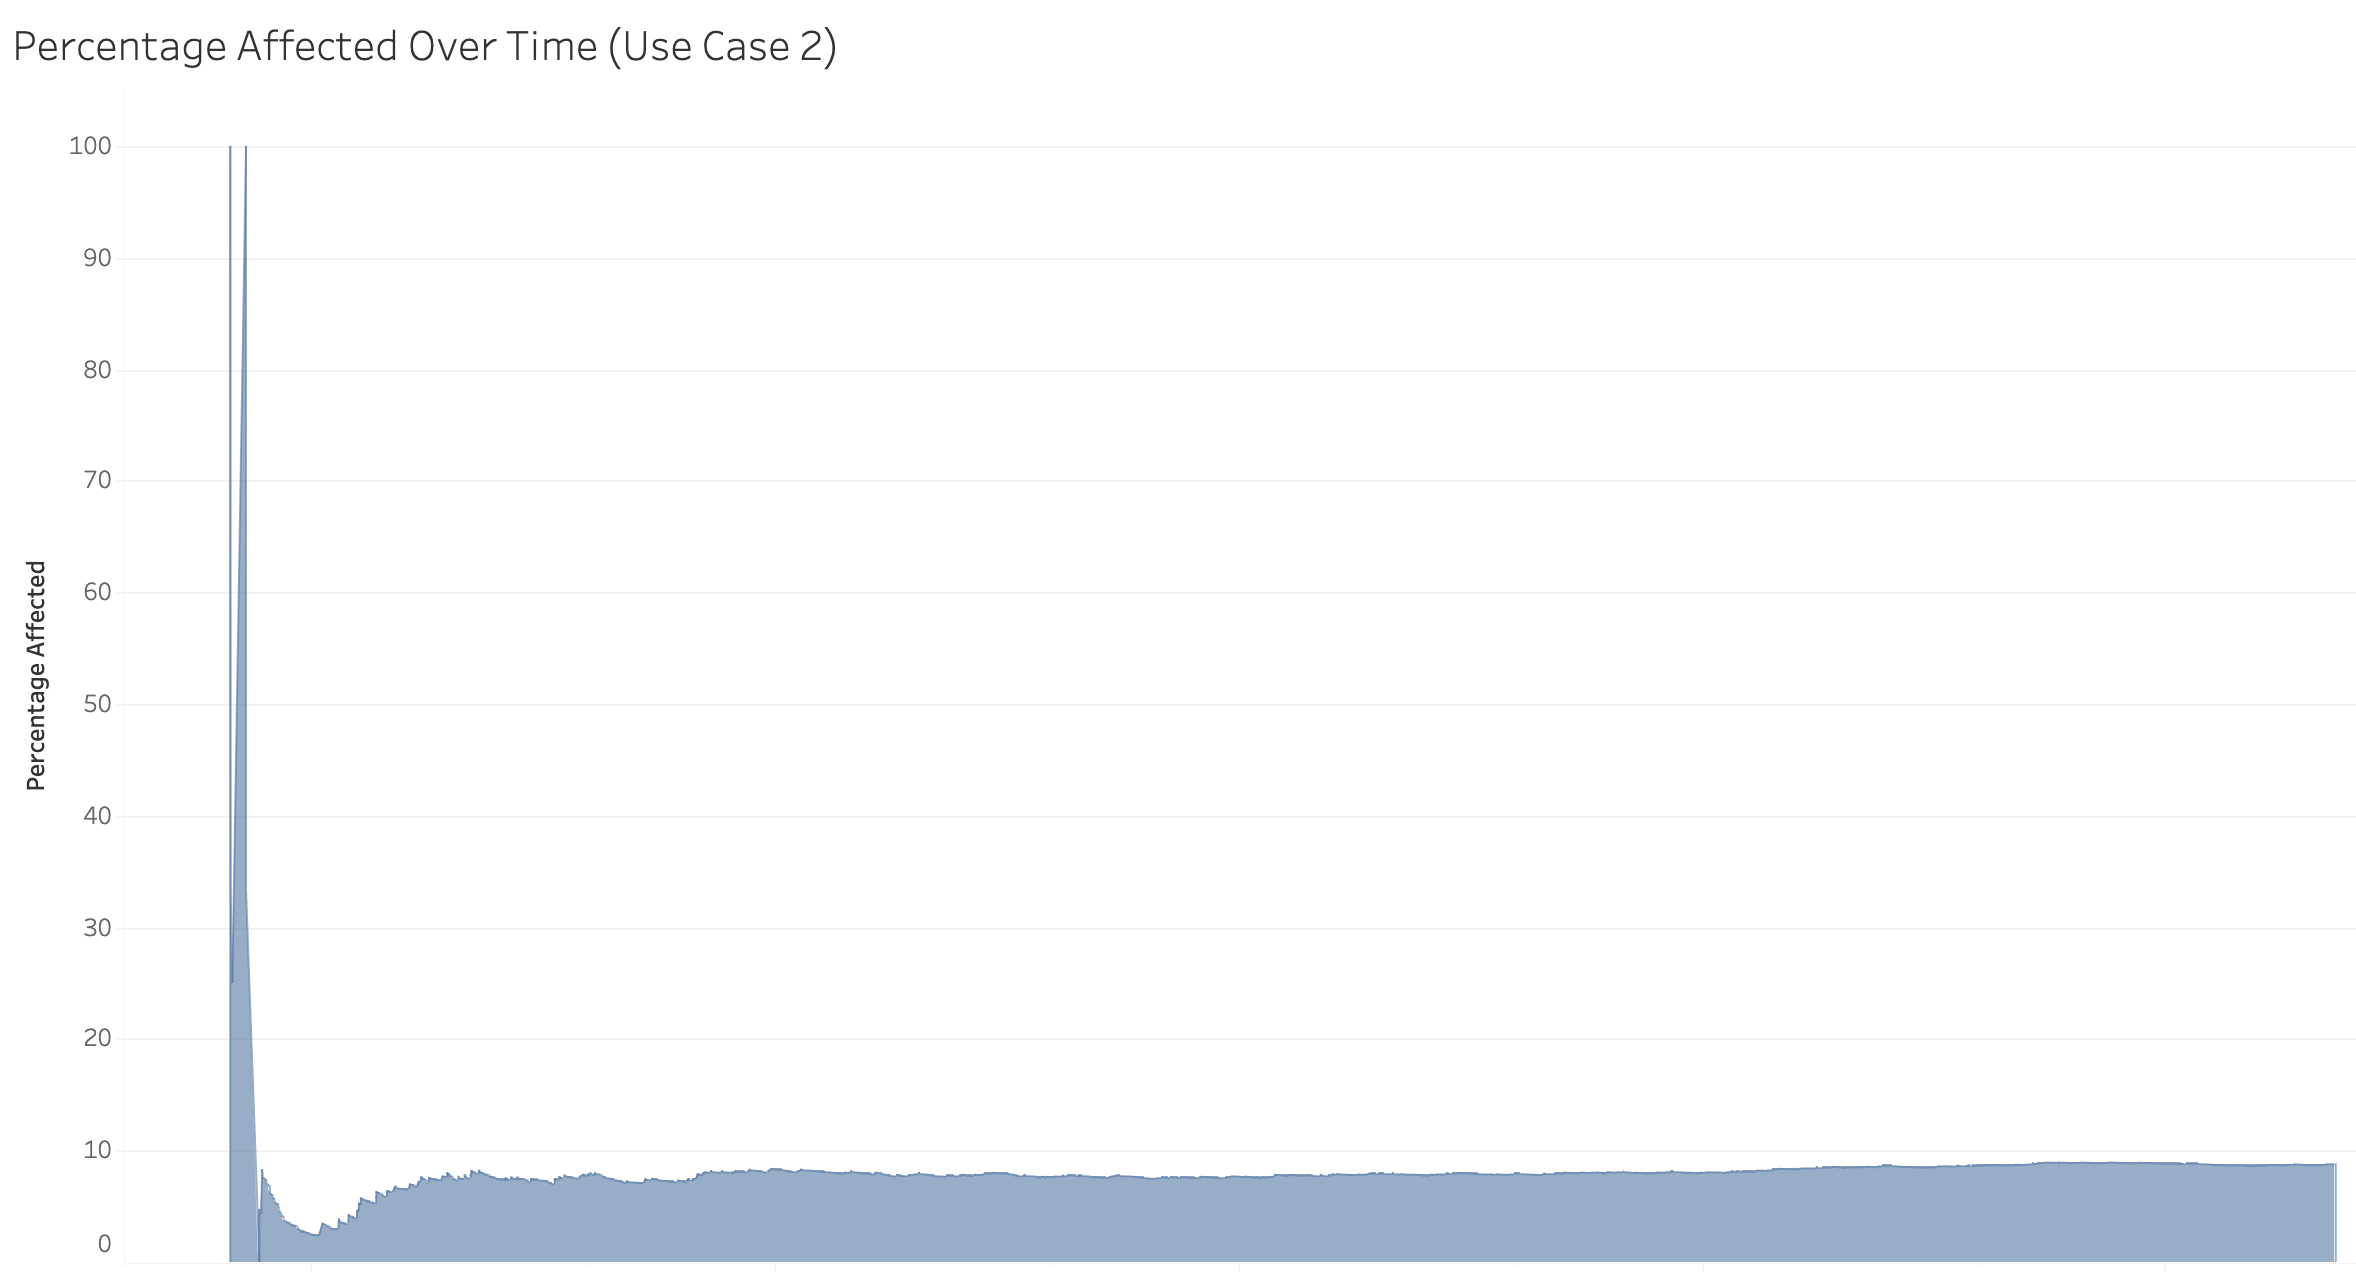
\includegraphics[scale=0.35]{images/UseCase2.png}
\caption{Use Case Beta}
\label{image:use_case_beta}
\end{figure}

After seeing the results from Use Case Beta we set the parameters of the next execution to be a bit more exaggerated. Use Case Gamma (shown in Figure \ref{image:use_case_gamma}) lowers the recalculation percentage to 5\% while the conflicting and abort percentages were set much higher at 40\%. This caused, that the affected transactions quickly spiked to 100\%; which kicked off a recalculation of the rankings within the system. After the recalculation the numbers are reset, but the conflicting and abort percentages are so high that the execution continues spiking the affected transactions to 100\%. This repetition of spikes continues throughout the entire execution. While Use Case Gamma is not an ideal system that transactions will execute within, it gave us a upper bound of what happens when there is a large percentage of affected transactions.

\begin{figure}
\centering
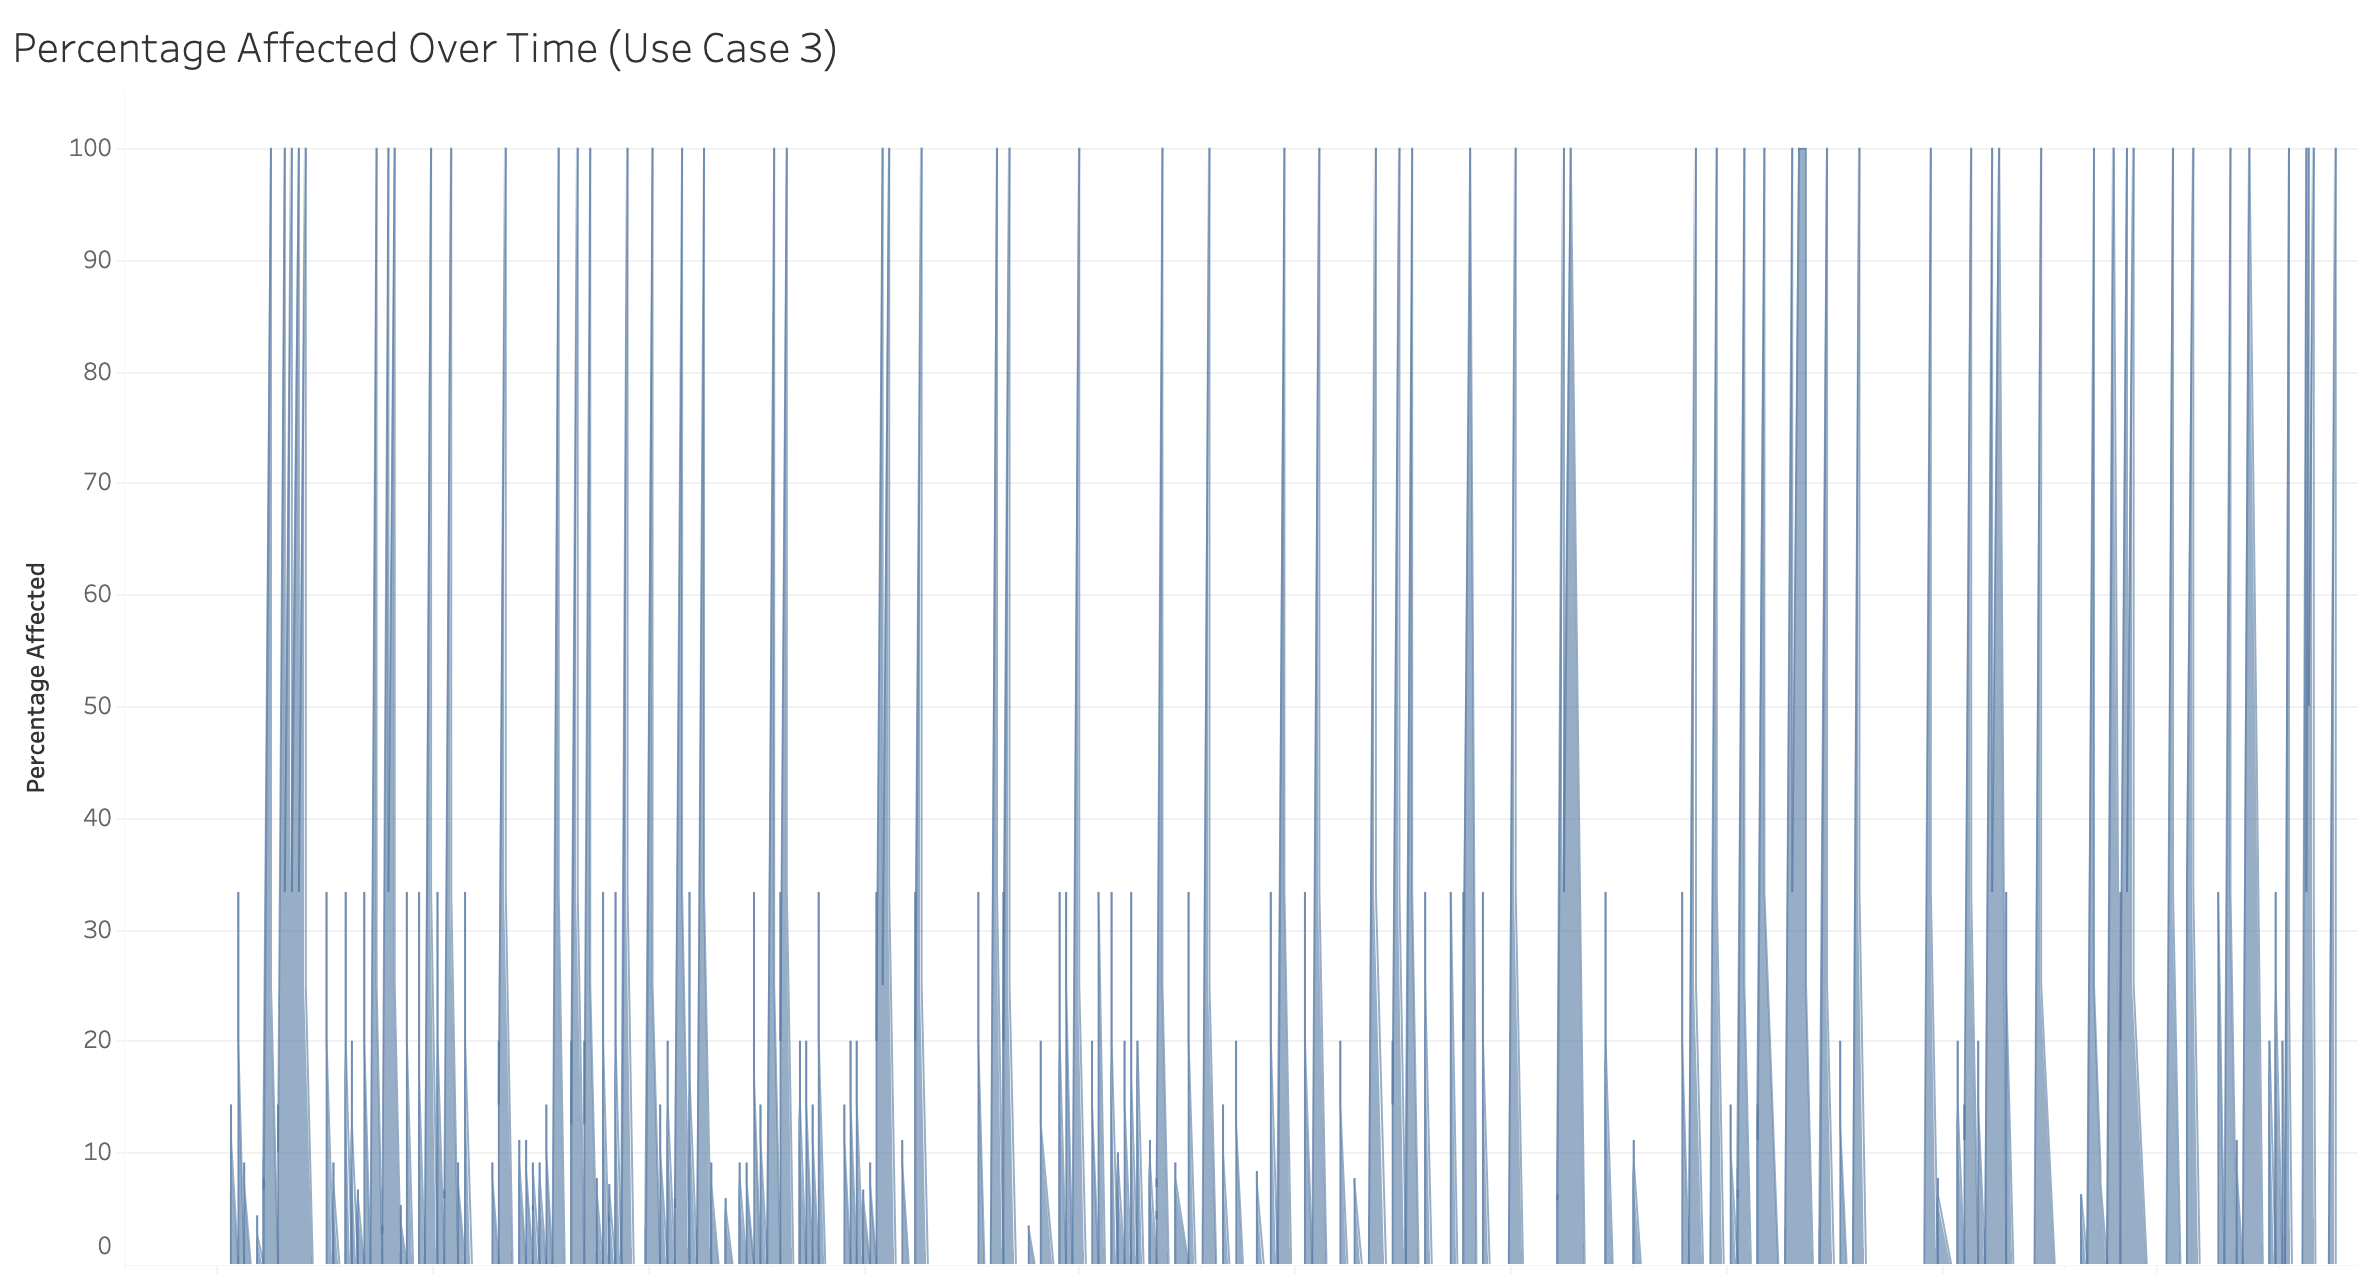
\includegraphics[scale=0.35]{images/UseCase3.png}
\caption{Use Case Gamma}
\label{image:use_case_gamma}
\end{figure}

The final use case of our initial executions was Use Case Delta (shown in Figure \ref{image:use_case_delta}). This use case is very similar to the previous use case and the results show that as well. In this use case we increase the recalculation percentage to 7\% while also increasing the conflicting and abort percentages to 50\%. There is nothing significant to note here other than the findings met our expectations for the given the parameters.

\begin{figure}
\centering
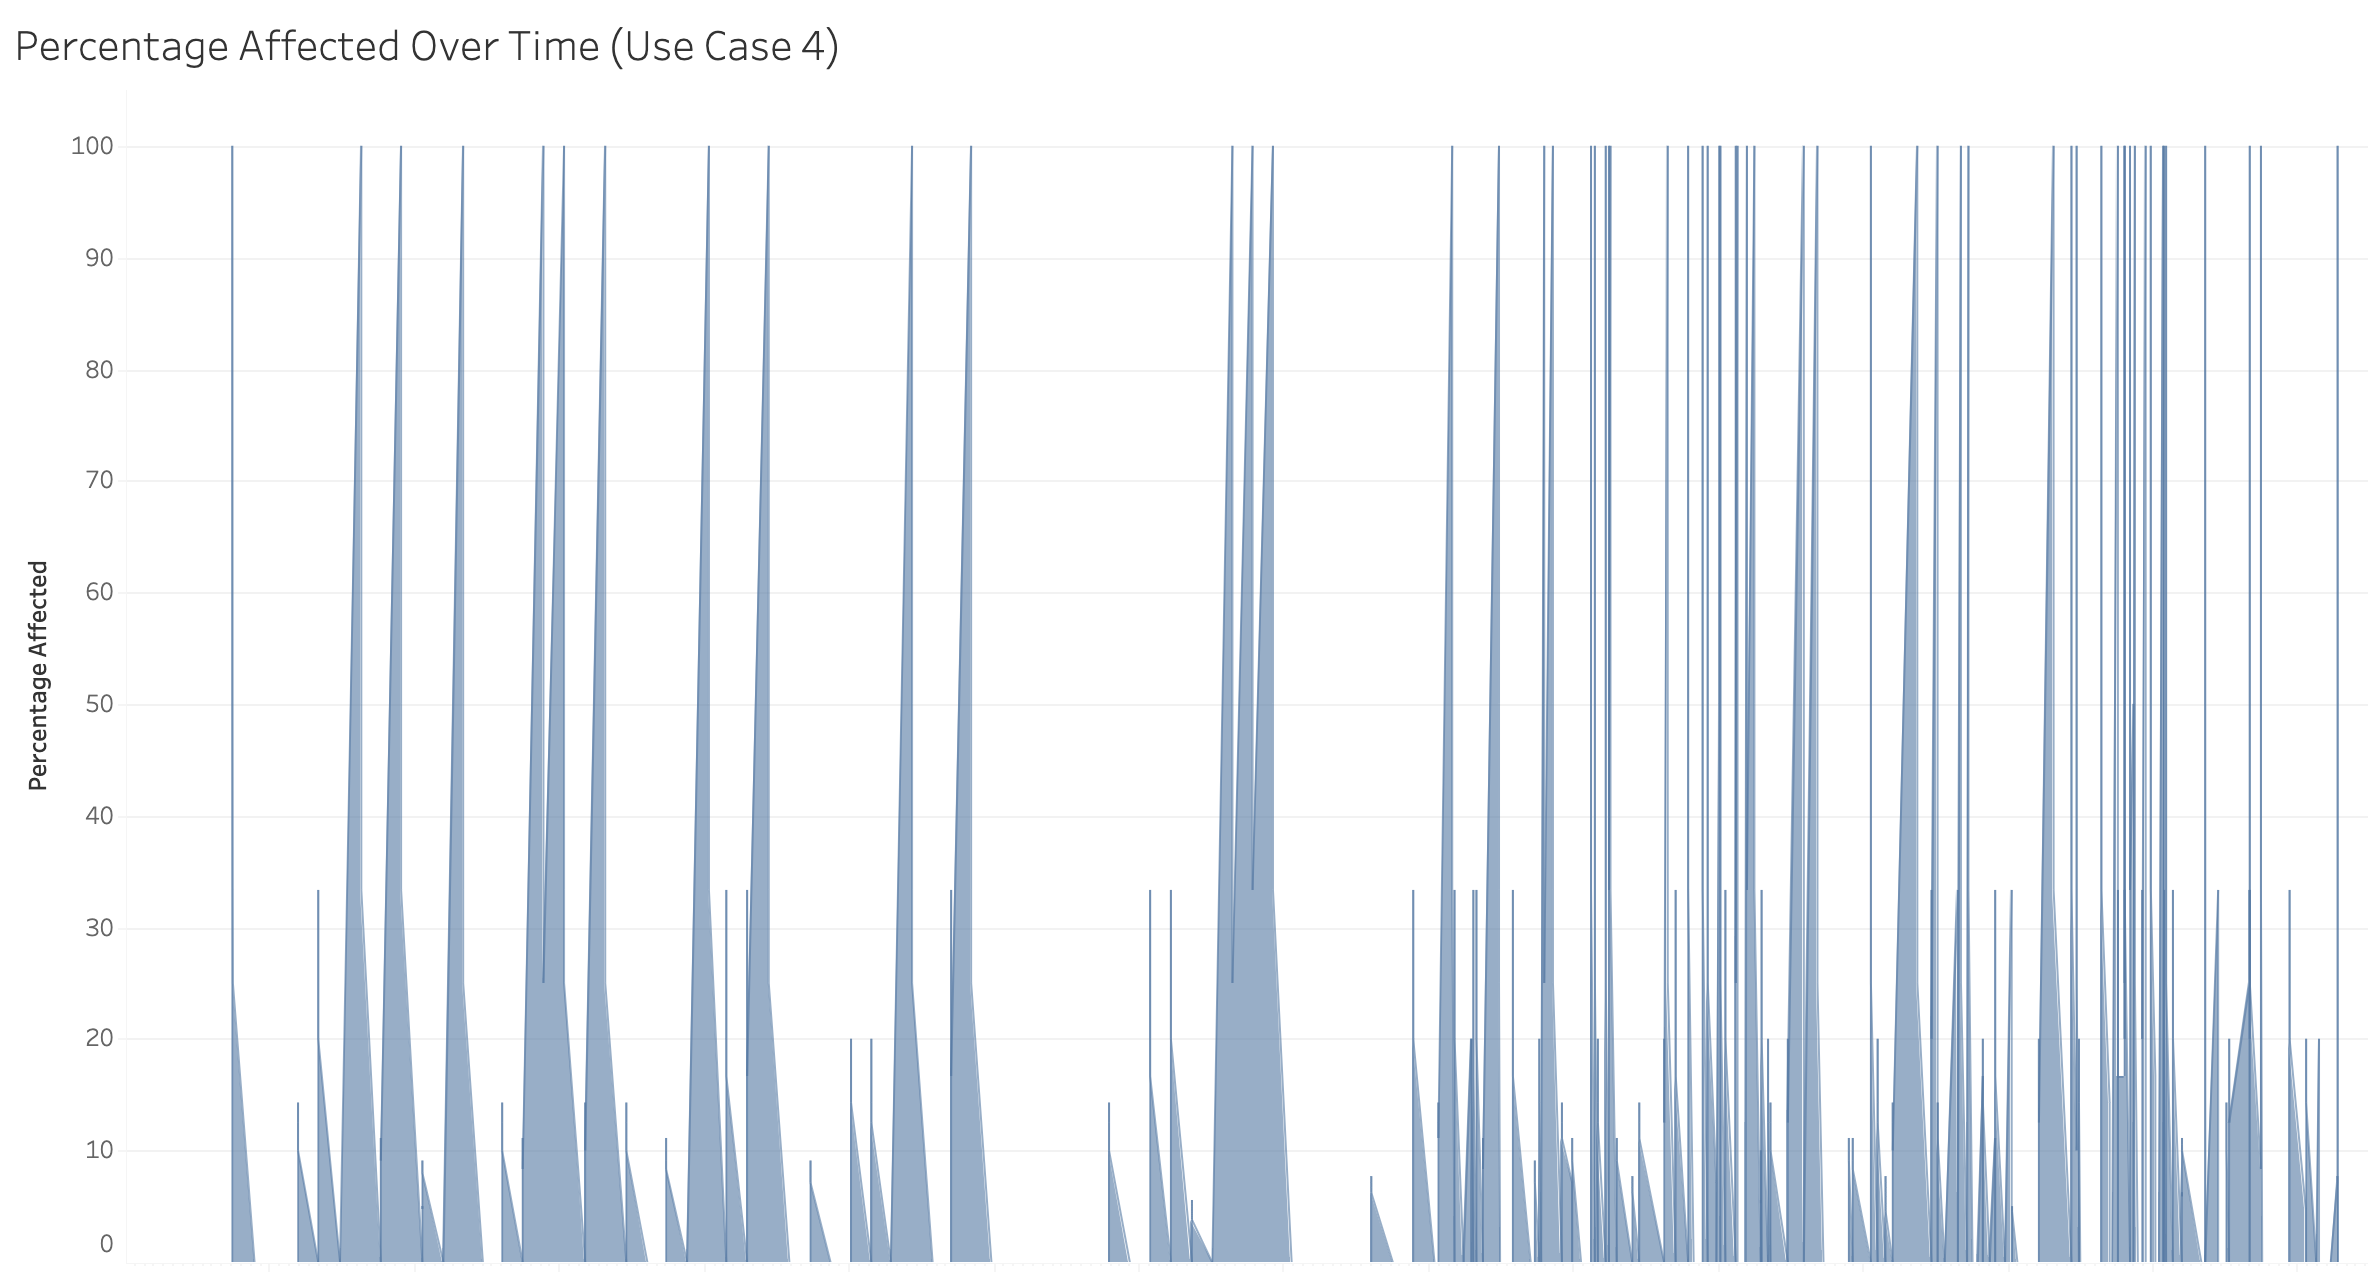
\includegraphics[scale=0.35]{images/UseCase4.png}
\caption{Use Case Delta}
\label{image:use_case_delta}
\end{figure}

After seeing the results of the preliminary use cases we formulated the use cases documented in Table \ref{tbl:use_cases}.
%to better verify our expectations in Section \ref{sec:anal_expectations}. 
In the next sections we present the use cases and our empirical results.
\subsection{Use Cases}
\label{sec:er_use_cases}

In this section, we discuss the use cases that were used to simulate executions within the schedulers. Input parameters collected as a set make up a single use case.

Use cases are the parameters used for a specific execution. Use cases have the following attributes

\begin{itemize}
    \item \textbf{Name}
    \begin{itemize}
        \item A simple name to uniquely identify the use case
    \end{itemize}
    \item \textbf{Total Transactions Executed}
    \begin{itemize}
        \item An integer representing how many transactions were executed within that use case
    \end{itemize}
    \item \textbf{Recalculation Percentage}
    \begin{itemize}
        \item This is a decimal number representing the percentage of aborted transactions over all transactions that is the threshold of when a recalculation should occur throughout the system
    \end{itemize}
    \item \textbf{Conflicting Percentage}
    \begin{itemize}
        \item This is a decimal number representing the percentage of transactions that will conflict during execution.
    \end{itemize}
    \item \textbf{Abort Percentage}
    \begin{itemize}
        \item This is a decimal number representing the percentage of transactions that will end in an abort during execution.
    \end{itemize}
\end{itemize}


These act as the input parameters for the executions as each set of use case parameters cause a different load on the system. The varying load consists of how many times a recalculation occurs and how many times a transaction must be executed again due to conflict or an abort. Table \ref{tbl:use_cases} shows the use case parameters that were used for simulation.

\begin{table}
\caption{Use Cases Executed}
\captionsetup{justification=centering}
\centering
 \begin{tabular}{|| c | c | c | c | c ||} 
 \hline
 \textbf{Name} & \textbf{Total \#} & \textbf{Recalculation \%} &  \textbf{Conflict \%} & \textbf{Abort \%} \\ [0.5ex] 
 \hline\hline
 Use Case 1 & 5,000 & 30 & 0 & 10  \\ 
 \hline
 Use Case 2 & 5,000 & 30 & 50 & 10  \\ 
 \hline
 Use Case 3 & 5,000 & 30 & 25 & 10  \\ 
 \hline
 Use Case 4 & 5,000 & 30 & 20 & 10  \\ 
 \hline
 Use Case 5 & 5,000 & 30 & 22 & 10  \\ 
 \hline
 Use Case 6 & 5,000 & 30 & 75 & 10  \\ 
 \hline
 Use Case 7 & 5,000 & 30 & 100 & 10  \\ 
 [1ex] 
 \hline
\end{tabular}
\label{tbl:use_cases} % label to refer figure in text
\end{table}

Before the use cases executed in Table \ref{tbl:use_cases} there were numerous use cases executed as discovery metrics for the best results generation. The use cases listed in Table \ref{tbl:use_cases} outline the optimal executions to outline our contribution.

In the next section we discuss how the experimentation was executed, limitations of the experimentation, and the goal of the experimentation.
\subsection{Execution}
\label{sec:er_execution}

The goal of this section is to provide clarity around the execution of the experimentation and outline the goal of the experimentation in regards to our contribution.

The experimentation discussed in Sections \ref{sec:er_application} and \ref{sec:er_use_cases} outlines the application architecture and the use cases used as a part of the execution to submit the solution to different workloads. The execution itself (shown in Figure \ref{image:flow_of_execution}) involves the execution of all four schedulers simultaneously with the same workload.

\begin{figure}
\centering
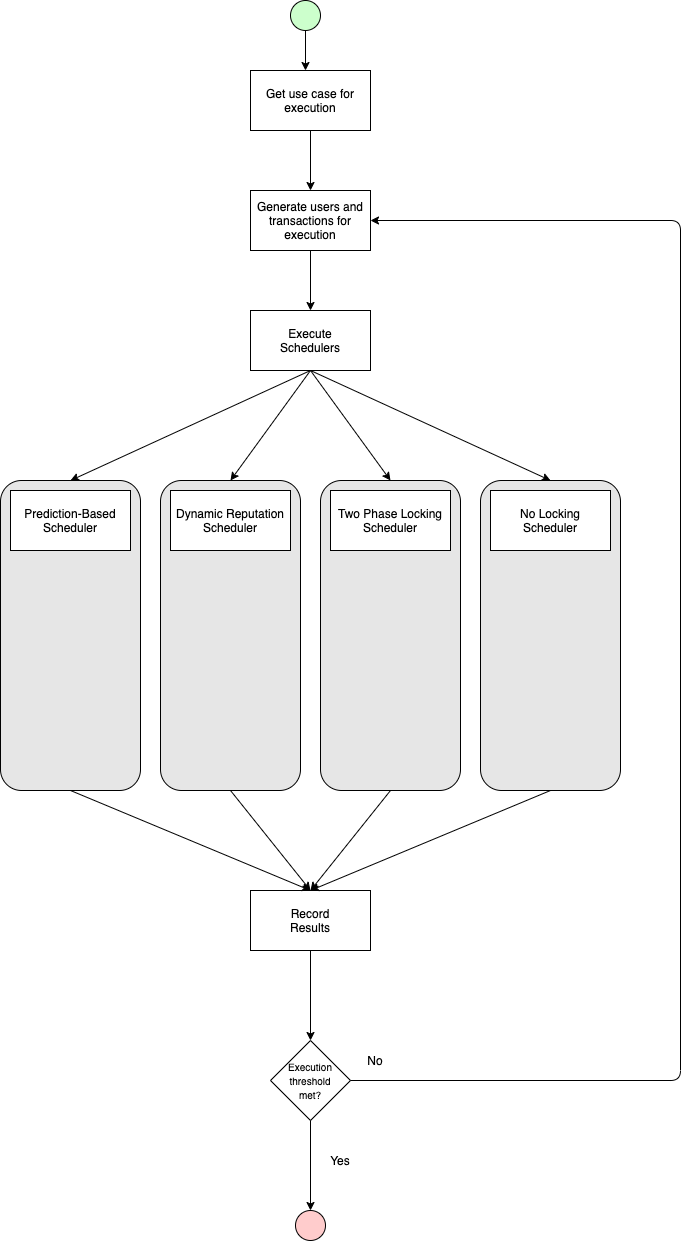
\includegraphics[scale=0.30]{images/Scheduler_Flow.png}
\caption{Flow of Execution}
\label{image:flow_of_execution}
\end{figure}

The primary limitation of the execution involves the number of transactions and users executed each time. The schedulers are not designed as fully functional schedulers that can accept multiple transactions and users but are subsets of the schedulers that only accept two users and two transactions each time. The primary goal of the scheduler executions is to validate the algorithms of the dynamic reputation scheduler among other comparative schedulers. Writing subsets of the schedulers that only accept pairs of transactions and users was much more feasible to implement as a prototype rather than a fully functional system. The flow of execution for the dynamic reputation scheduler is outlined in Figure \ref{image:flow_of_drs} and the flow of the prediction based scheduler implemented in our previous work (see \cite{ravan_ensuring_2020}) is outlined in Figure \ref{image:flow_of_pbs}. The \gls{2pl} and NoSQL schedulers implement the standard algorithms that are defined.

\begin{figure}
\centering
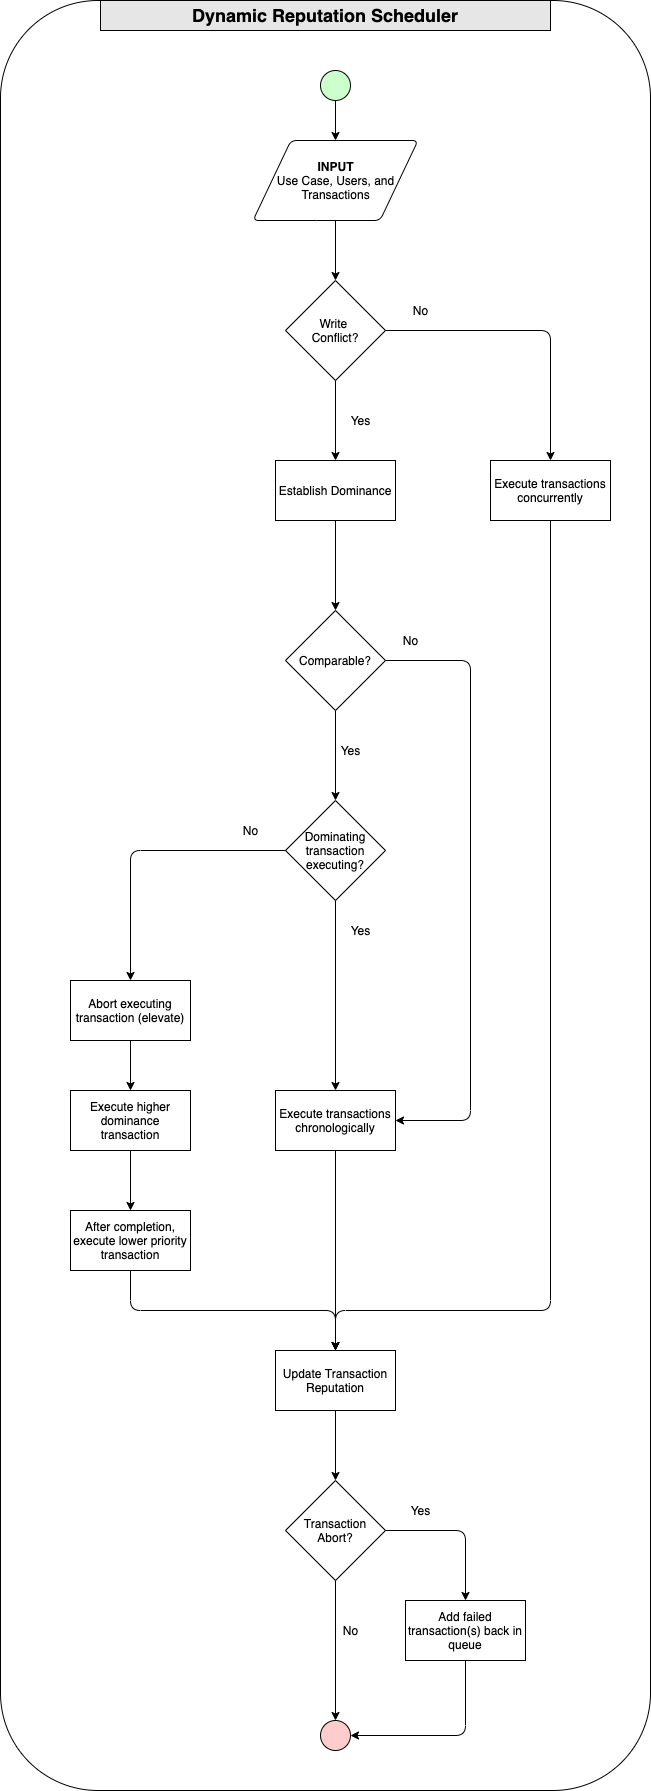
\includegraphics[scale=0.28]{images/DRPScheduler.png}
\caption{Flow of Dynamic Reputation Scheduler}
\label{image:flow_of_drs}
\end{figure}

\begin{figure}
\centering
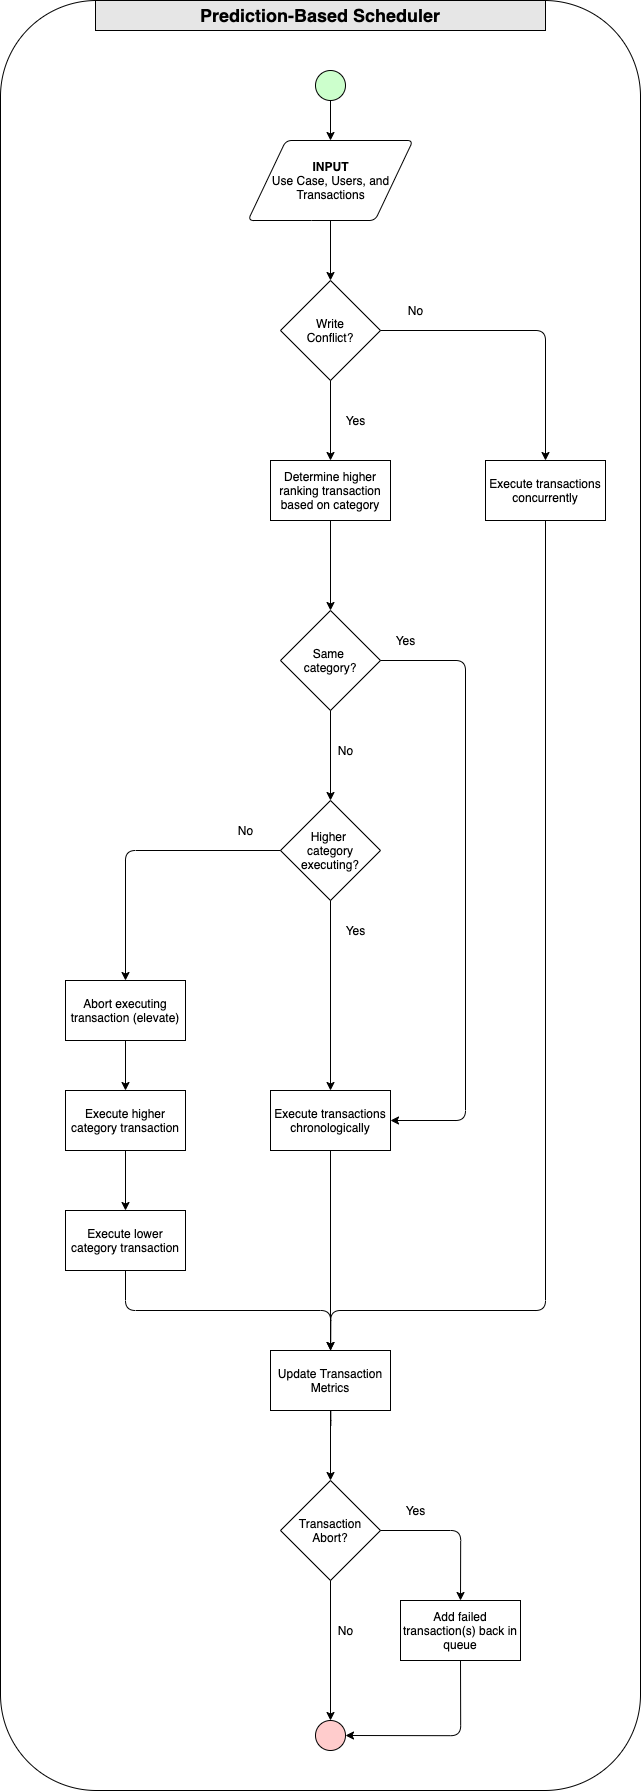
\includegraphics[scale=0.28]{images/PBSScheduler.png}
\caption{Flow of Prediction Based Scheduler}
\label{image:flow_of_pbs}
\end{figure}
\section{Analysis}
\label{sec:analysis}

When looking at the behavior of all the use case executions we did notice trends given the parameters that were used.

Use Cases 1 and 2 performed very similar with the parameters given. In both use cases, the number of aborted transactions never reached above 10\% of the total transactions therefore a recalculation of rankings was never executed. As more transactions executed within the system, the more the percentage of aborted transactions plateaued and we never saw a recalculation take place.

Use Cases 3 \& 4 were purposely executed with extreme parameters in order to see the load the system would endure with multiple recalculations. There were multiple recalculations executed in asynchronous threads. The executions did not block the execution of the transactions but caused a great deal of CPU usage. These are parameters that we would not expect in a live system but were used specifically to see the load of recalculations.

Use Cases 5 \& 6 were the use cases where all three schedulers were executing. All three schedulers executed with the same transactions, users, and use case parameters to get an equal comparison. This was the best indicator of what would be expected in a real world scenario.
\subsection{Expectations}
\label{sec:anal_expectations}

Before executing the simulation, our definitions (see Section \ref{sec:definitions}) and system model (see Section \ref{sec:system_model}) led us to certain expectations that would come from the simulation. The overall expectation and claim from the dynamic reputation solution is that it provides a low overhead resource management solution with consistent scheduling. That claim is supported by the following three expectations:

\begin{enumerate}
    \item There will be greater reward and punishment from the dynamic reputation solution than from our previous prediction-based solution
    \item We will see the reward and punishment reflected in the rankings of the users and transactions
    \item The execution time will be comparable to both the previous prediction-based and \gls{2pl} scheduler to not indicate a serious overhead
\end{enumerate}
\subsection{Findings}
\label{sec:anal_findings}

Our first finding defends our first claim that there will be greater reward and punishment in our new solution than our previous prediction-based solution. We can determine a greater level of reward and punishment by looking at the percentage of transactions that were elevated due to a conflict. Our formula for calculating the percentage of elevated transactions is below:

\[\textrm{$T_{elevate}$} = \textrm{\# of executions that caused an ELEVATE}\]
\[\textrm{$T_{total}$} = \textrm{Total \# of executions}\]
\[\textrm{$P_{reward}$} =\frac{\textrm{$T_{elevate}$}}{\textrm{$T_{total}$}} \times 100\]
 
After analyzing the results we discovered that the $P_{reward}$ for the dynamic reputation solution is 51.9\% and the $P_{reward}$ for the prediction-based solution is 7.1\%. This is expected given that the reputation management solution involves a much more granular approach to establishing dominance that the four category system in the previous prediction-based solution. Therefore, this confirms that the dynamic reputation solution allows for a greater percentage of reward and punishment among the conflicting transactions.

Our second finding defends our second claim that we will see the reward and punishment reflected in the rankings of the users and transactions. By seeing a variance in the rankings of the users and transactions (see Definitions \ref{def:commit_ranking}, \ref{def:efficiency_ranking}, \ref{def:user_ranking},  and \ref{def:system_abort_ranking}) then we can confirm that our recalculations are causing changes in dominance based on the reputations of users and transactions. Figure \ref{image:variance_of_transaction_rankings} and \ref{image:variance_of_user_rankings} are two graphs showing the variance in the growth/reduction of transaction and user rankings across executions. You can see the rankings shrinking and growing as recalculations occur. Figure \ref{image:variance_of_transaction_rankings} shows the transaction rankings changing throughout the system. The y-axis represents the variance. The x-axis is the transaction ID (not shown for view ability). This graph represents all transactions that executed more than once within the system in order to show the changes in rankings between executions.

Figure \ref{image:variance_of_user_rankings} shows the same variance but for user rankings as they change throughout the system due to recalculation. The graph shows that the reward and punishment is actively being applied throughout the system.

\begin{figure}
\centering
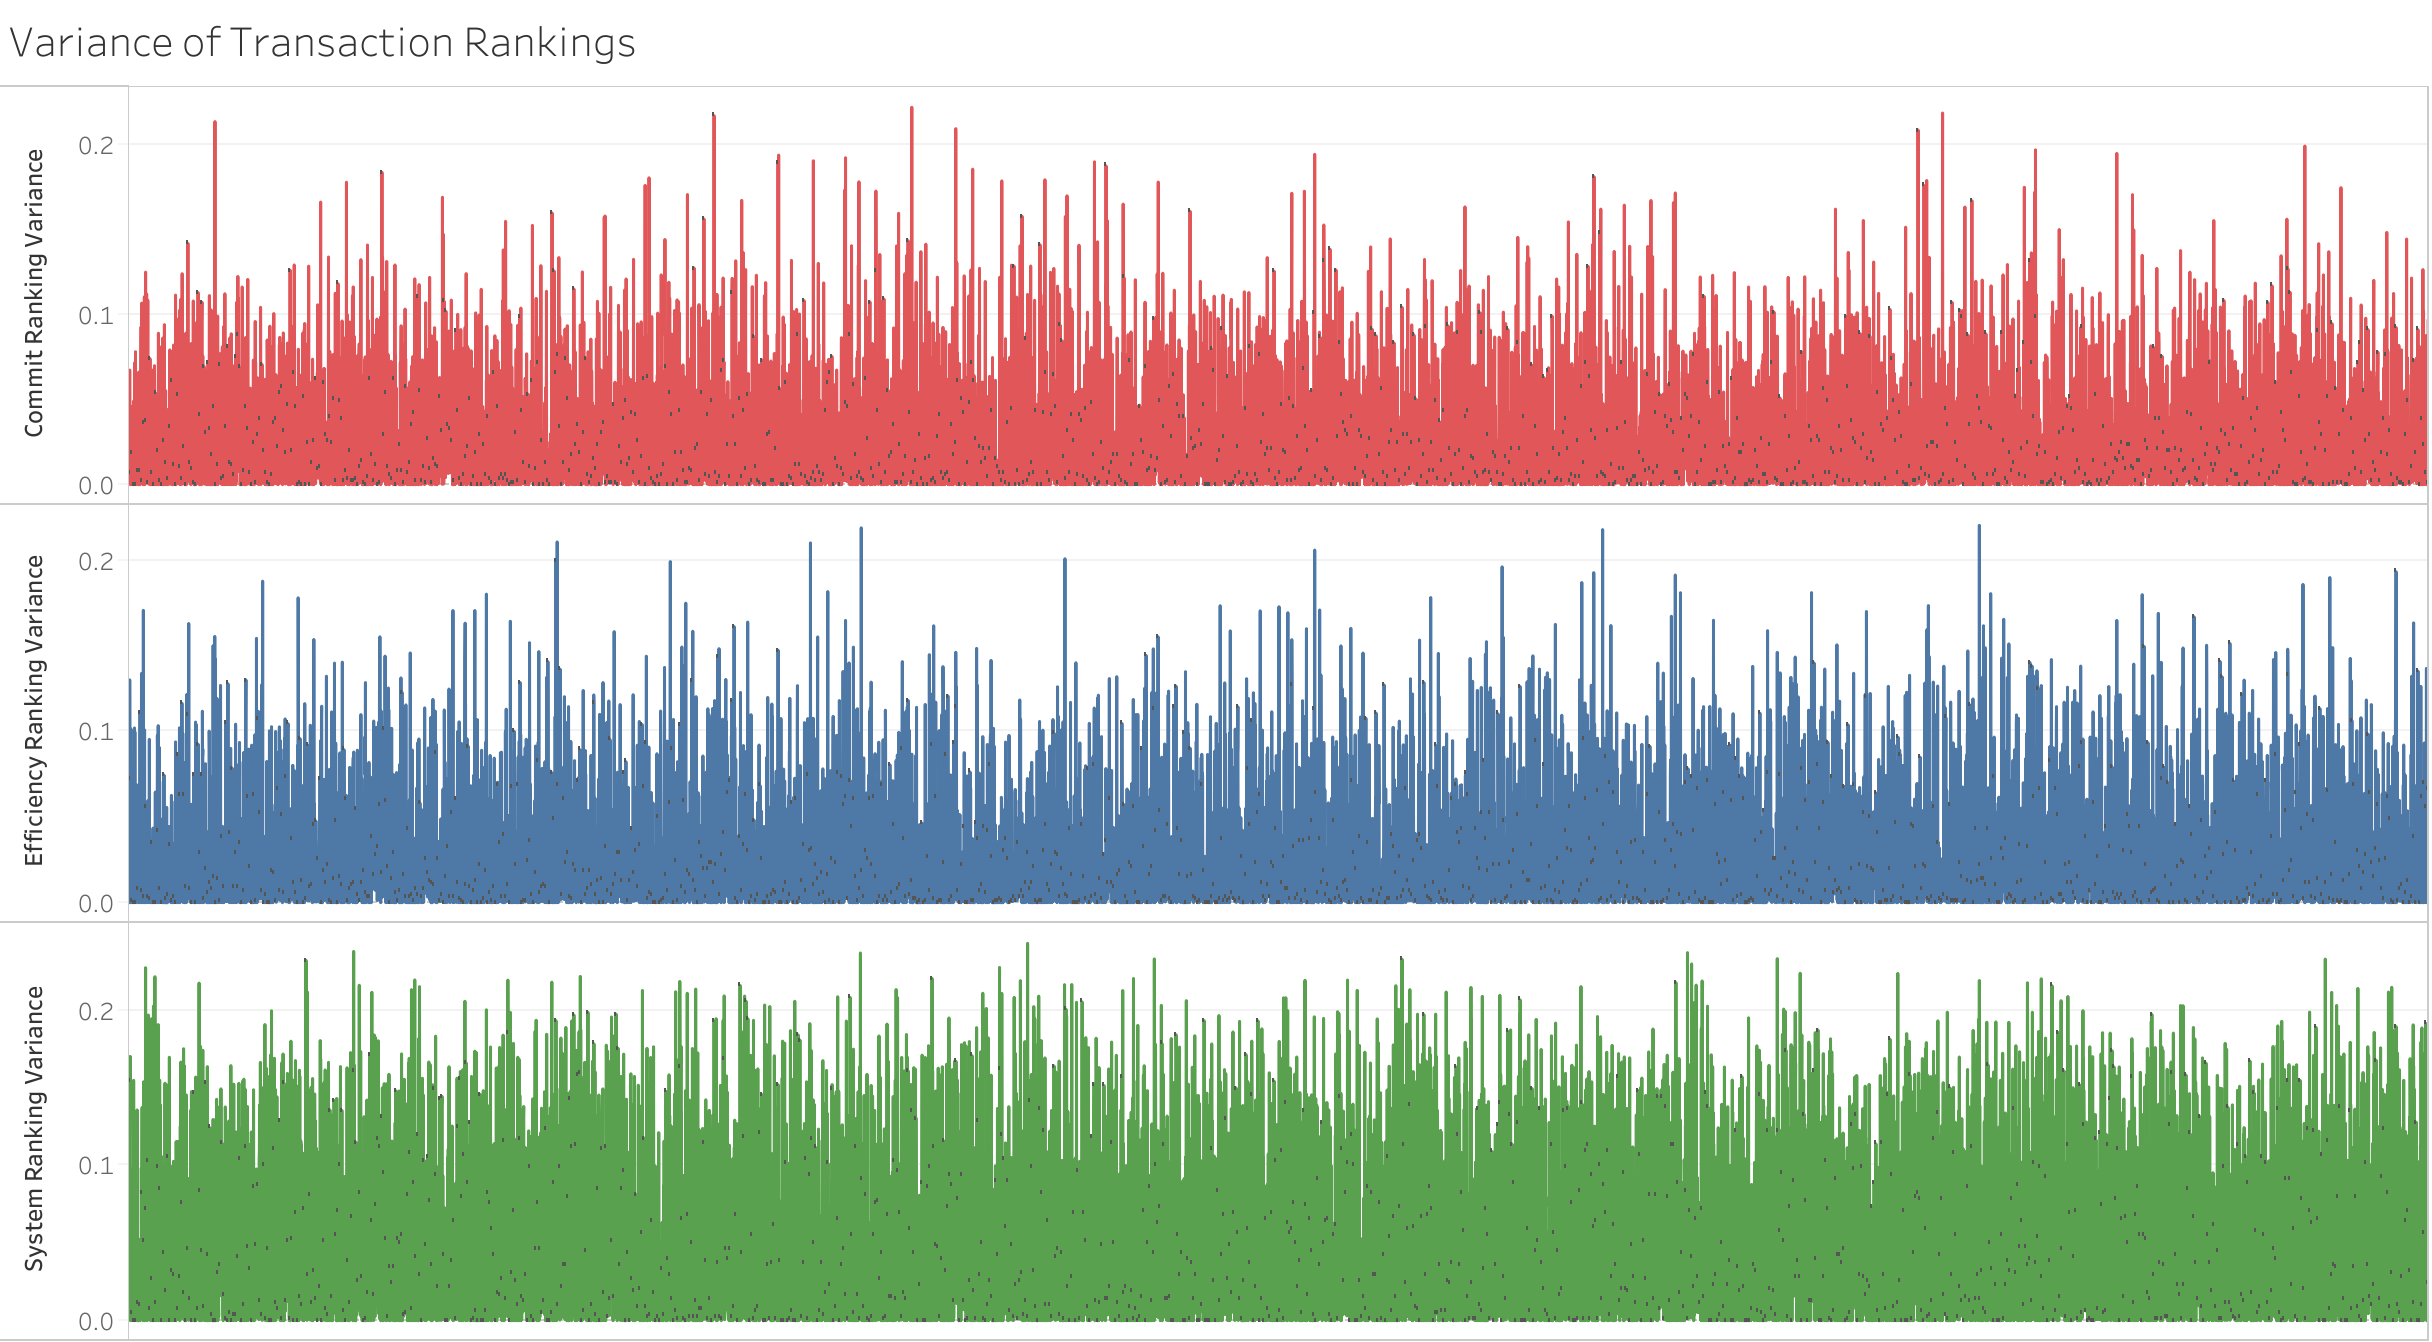
\includegraphics[scale=0.20]{images/VarianceofTransactionRankings.png}
\caption{Variance of Transaction Rankings}
\label{image:variance_of_transaction_rankings}
\end{figure}

\begin{figure}
\centering
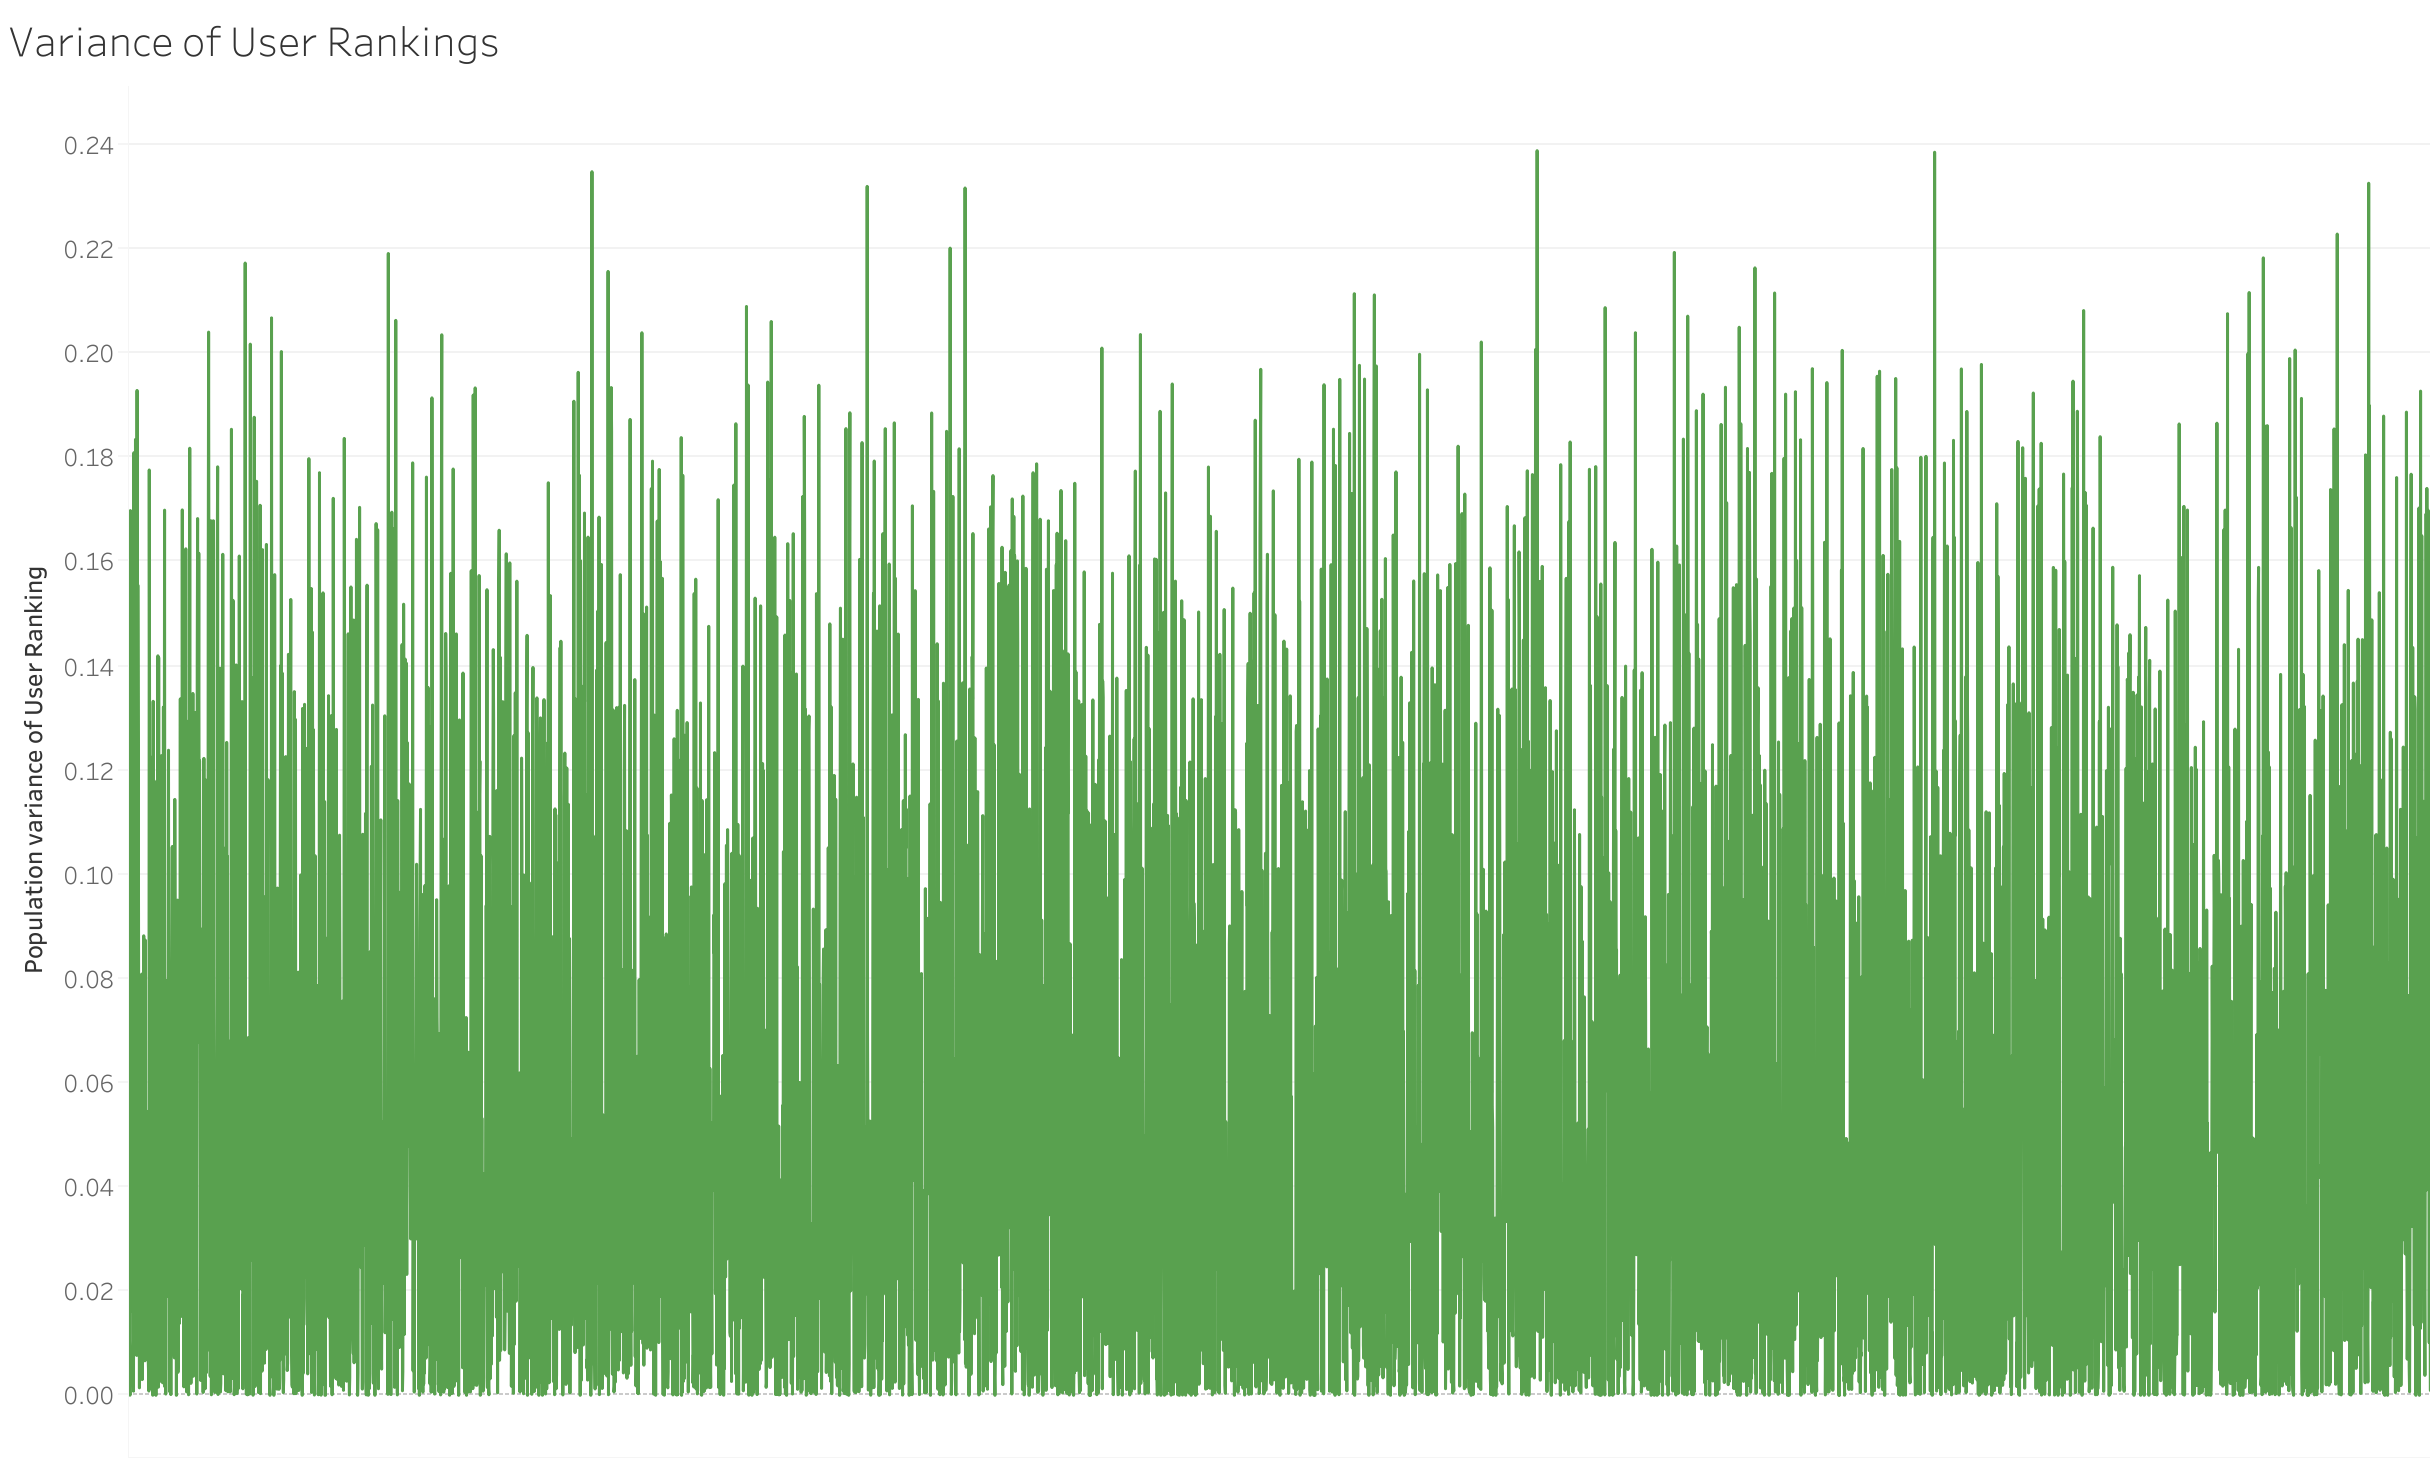
\includegraphics[scale=0.20]{images/VarianceofUserRankings.png}
\caption{Variance of User Rankings}
\label{image:variance_of_user_rankings}
\end{figure}

Our third and final finding defends our third claim that the execution time will be comparable to both the previous prediction-based and \ac{2PL} schedulers. When comparing all of the schedulers execution time over different workloads (see Figure \ref{image:scheduler_comparison}) we can see the differing execution times however, even with the differing execution times the overhead of the dynamic reputation system is comparable and a feasible solution. This defends our third and final claim that the dynamic reputation solution is a feasible solution but as we examine the data we can be more precise of when the solution should be legitimately considered.

After examining the data we see that the execution time is directly related to the workload. The defining difference of the workloads is the percentage of conflicting transactions in the workload. As the percentage of conflict increases in the differing workloads you can see the schedulers begin to execute at different execution times. 

From the graph in Figure \ref{image:scheduler_comparison} we can deduce that the best environment for the dynamic reputation solution is within execution environments that contain greater than 20\% conflicting transactions. Execution environments with high levels of conflict can benefit from the dynamic reputation solution while environments with less than 20\% conflict would be impacted by the overhead of processing within the dynamic reputation solution.

\begin{figure}
\centering
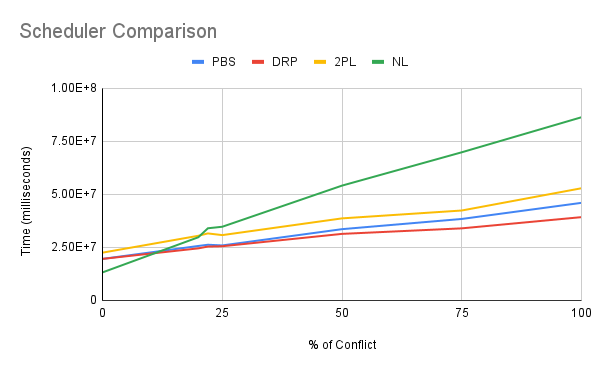
\includegraphics[scale=0.60]{images/SchedulerComparison.png}
\caption{Scheduler Comparison}
\label{image:scheduler_comparison}
\end{figure}

With our findings defending all three of our claims we can with confidence claim that the dynamic reputation solution provides a low overhead resource management solution with consistent scheduling.

\section{Conclusion}
\label{sec:conclusion}

% In closing we conclude that this extension of the prediction-based scheduling solution involves the identification of two unique problems: identifying a class of transactions and maintaining a dynamic reputation for that class of transactions. Identifying a class of transactions allows PBS the ability to assign a categorization to transactions with common intrinsic attributes. Separating the intrinsic attributes from the extrinsic involves a flyweight modeling approach in order to properly model transaction classes. 

In closing we conclude that the dynamic reputation solution provides a system of greater reward and punishment than the previous prediction-based solution. The four category system of the prediction-based solution doesn't contain the level of granularity needed to establish dominance in conflicting situations. We also conclude that the overhead of the dynamic reputation solution is comparable to the previous prediction-based and \gls{2pl} solutions therefore establishing a resource management solution with a feasible overhead and consistent scheduling. By analyzing our findings from the experimentation we can conclude that execution environments with workloads of greater than 20\% conflicting transactions would benefit from the granularity of the dynamic reputation scheduler to provided consistency and efficient scheduling. %% Chapter 3
% \chapter{Dissertation Outline}
\label{chap:outline}

In this chapter we explain the full dissertation outline of milestones that were accomplished and their timing.

% \section{Introduction}
\label{diss:introduction}

The work needed for completion involves two problems that build upon the foundation of the existing work. In this chapter, we explain in detail the components needed for the completion of work. The first component is extending the prediction-based solution to multi-level secure databases by transitioning to a three-dimensional decision matrix. The second and final component is the work needed to dynamically manage the reputation of transactions executed within a prediction-based scheduler. We propose that a complete solution including both MLS databases and dynamic transaction reputation would satisfy all requirements needed for a Ph.D. All extensions listed in previous chapters will work towards prototypes for each problem in order to gather empirical results that prove the soundness of each solution.

% \input{chapters/5__Dissertation_Outline/sections/mls_databases}
% \input{chapters/5__Dissertation_Outline/sections/dynamic_reputation}
% \section{Prediction-Based Scheduling within Linked Databases}
\label{diss:linked_databases}

In this section we discuss the proposed work for implementing the comprehensive prediction-based scheduler (Chapters \ref{chap:prediction_based_scheduler} \& \ref{chap:multi_level_security}) into a linked-database environment. This section contains the proposal itself. The background information, problem definition, and existing research for the problem is outlined in Chapter \ref{chap:pbs_w_link_db}.

The final problem to attempt is the adaptation of the Prediction-based solution within a linked database environment. The challenges of scaling the solution to a linked database environment still needs to researched and the problems defined so that a proper solution can be presented. We believe there is a problem to be formally defined and analyzed through the lens of the Prediction-based solution.

Our proposal for linked database systems is much like the proposal outline in Section \ref{proposal:mls_database_scheduling}. Again, we propose researching the current academic environment for what is common practice among linked database systems, providing a solution based on the outcome of that research, verifying the accuracy, and working toward a viable prototype with initial results. Once again, since the bulk of the theoretical and simulation results have been accomplished in Chapter \ref{chap:prediction_based_scheduler} through the publication of \cite{ravan_ensuring_2020} we propose that this work consist of a submission to a conference.
\section{Dissertation Outline}
\label{diss:dissertation_outline}

\newcommand{\dissPhaseOne}
{\textbf{Transactional Correctness:} Consistency control algorithms prototyped and formally proven as a part of prediction-based solution (\gls{pbs}). \textbf{Published in IEEE Transactions, February 2020}\newline}

\newcommand{\dissPhaseTwo}
{\textbf{Dissertation Proposal}}

\newcommand{\dissPhaseThree}
{\textbf{Dynamic Transaction Reputation:} Analyze and leverage reputation management solutions within \gls{pbs} \textbf{Submitted to ACM Transactions of Information Systems\newline}}

\newcommand{\dissPhaseFour}
{\textbf{Database Recovery using Provenance:} Assisted with publication with other students. \textbf{Published in Data 2021} }

\newcommand{\dissPhaseFive}
{\textbf{Dissertation Defense}}


Table \ref{table:dissertation_outline} shows the dissertation in all of its phases. Research began in August of 2014 after becoming enrolled as a student. I met with Dr. Farkas initially and began working on the transactional-correctness portion of the work that transitioned into the prediction-based scheduler. This is the work detailed in Chapter \ref{chap:prediction_based_scheduler}. The work underwent multiple revisions until we were confident with the solution and the form it has now taken. The work was completed and submitted to IEEE Transactions on Services Computing in April of 2019. In January of 2020, we received a decision of Accepted with Minor Revisions. Revisions were made and that has now been published. This serves as the bulk of the work and also the foundation of the extensions proposed in Chapters \ref{chap:future_work}. Afterwards I assisted with another work regarding using provenance as a database recovery mechanism. This work was published in July of 2021 (see \cite{theppatorn_2021}).Prior to that in February of 2020, we begin work on the dynamic transaction reputations. That work was completed in August of 2021 and submitted to ACM Transactions on Information Systems. We are still awaiting response.

\begin{table}
\centering
\renewcommand\arraystretch{1.4}
\captionsetup{singlelinecheck=false, labelfont=sc, labelsep=quad, justification=centering}
\caption{Outline}\vskip -1.5ex
\begin{tabular}{@{\,}r <{\hskip 2pt} !{\foo} >{\raggedright\arraybackslash}p{10cm}}
\toprule
\addlinespace[1.5ex]
February 2020 & \dissPhaseOne\\
August 2020 & \dissPhaseTwo\\
September 2020 & \dissPhaseThree\\
July 2021 & \dissPhaseFour\\
November 2021 & \dissPhaseFive\\
\end{tabular}
\label{table:dissertation_outline}
\end{table}
\section{Concluding Remarks}
\label{proposal:conclusion}

The outline in Table \ref{table:dissertation_outline} contains major milestones that are apart of the dissertation path. Minor milestones, revisions, direction changes, and personal milestones have been omitted as they are not relevant to the completion of the dissertation. %% Chapter 4
\chapter{Future Work}\label{chap:future_work}

In this Chapter we discuss the potential for future work and extensions of the prediction-based scheduler. Primarily we discuss the work involved with multi-level secure databases.

\section{Introduction}
\label{mls:introduction}

Now that the framework for transactional correctness has been developed (work published in \cite{ravan_ensuring_2020}) within the prediction-based solution there is potential to extend the reputation score of the prediction-based scheduler to a categorization for multi-level secure database. The added attribute to the reputation score would include the security classification and allow for a much more robust decision-model. This portion of the overall solution would focus on multi-level secure database systems and covert timing channels. By providing an additional attribute to the existing framework we can therefore extend our reputation score to include security levels. This allows us to provide a cover story for the timing difference of transactions with differing security classifications. 

The problem with multi-level secure databases is the possibility that there could be a covert channel allowing unauthorized access. The covert channel would provided the ability for a transaction of a lower security classification to access resources designed for a higher security classification. Existing research provides possible solutions but many of the solutions starve transactions of higher security classifications from gaining access to the resources needed (see Section \ref{mls:related_work}). With that cover story in mind we can then provide a solution that elevates high security transactions would the presence of a covert timing channel. With the prediction-based solution provided in Chapter \ref{chap:prediction_based_scheduler} and the reputation score provided in Chapter \ref{chap:dynamic_reputation}, we can provide a cover story that determines locking priority based on the reputation of the transaction as a whole. This prevents the starvation of higher security classification transactions. By taking into consideration the security classification as a metric to calculate the reputation of the transaction, we also prevent the presence of covert channels. 
\section{Problem Definition}
\label{mls:problem_definition}

Multi-level secure databases (referred to as \ac{MLS} databases going forward) differ from traditional databases in that there is content within the database that cannot be accessed by all users of the database. There is data within the database itself that contains a high security classification (or multiple security classifications) than other data. This is also more volatile than multi-tenant systems. Multi-tenant systems also contain data which cannot be accessed by all users, but the data within the system contains the same priority when it comes to transaction scheduling. Security classifications within \ac{MLS} databases introduce priorities and therefore introduce the issues of starvation. \ac{MLS} databases also introduce the issue of covert channels since there are multiple security classifications. 

A covert channel is a channel of communication that performs communication outside of the normal access control mechanisms. This then makes it very hard to to secure using existing security measures since normal security measures are performed on the existing access control mechanisms. There are two main types of covert channels; storage channels and timing channels. Storage channels are a form of communication by modifying an existing storage location with data that would normally not be detected. Timing channels expose security issues by the presence or absence of a delay in transaction processing. Figure \ref{fig:covert_channel_exposure} shows the time delay difference between a normal operating system load to that of a delayed load operation. This presence of a time delay can allow for information passing to occur and the attacker to infer components of the system architecture especially in \ac{MLS} databases.

\begin{figure}
\centering
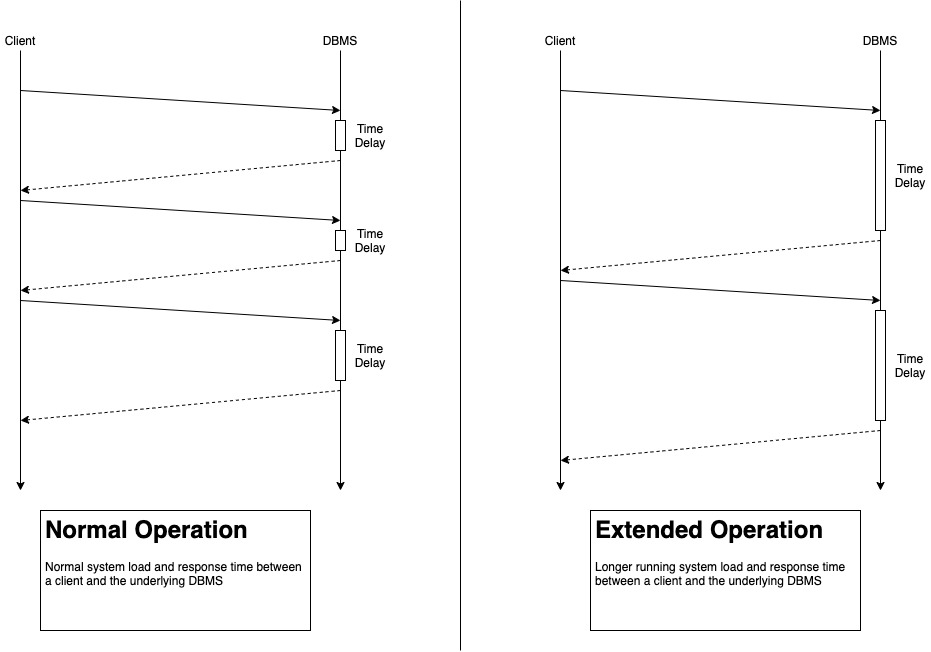
\includegraphics[scale=0.45]{images/CovertTimingChannel.jpg}
\caption{Covert Channel Exposure}
\label{fig:covert_channel_exposure}
\end{figure}

In order to prevent a timing covert channel within \ac{MLS} database systems, there must not be a presence of a timing delay for transactions with lower security classifications. The transactions must incur the standard time delay as a normal transaction so that there is no suspicion that a covert channel is available.

\subsection{Elevating The Priority}
\label{mls:problem_definition_elevation}
Most concurrency control algorithms solve this issue by giving a sort of precedence or priority to lower security classification transactions to prevent any time delay. However, this can cause issues with transactions with a higher security classifications if high security transactions continually conflict with lower transactions. The high security transactions can suffer from starvation and cause a huge performance hit. Figure \ref{fig:ws_trans_starvation} shows an example of how a high security classification transaction can experience starvation with standard locking mechanisms.

\begin{figure}
\centering
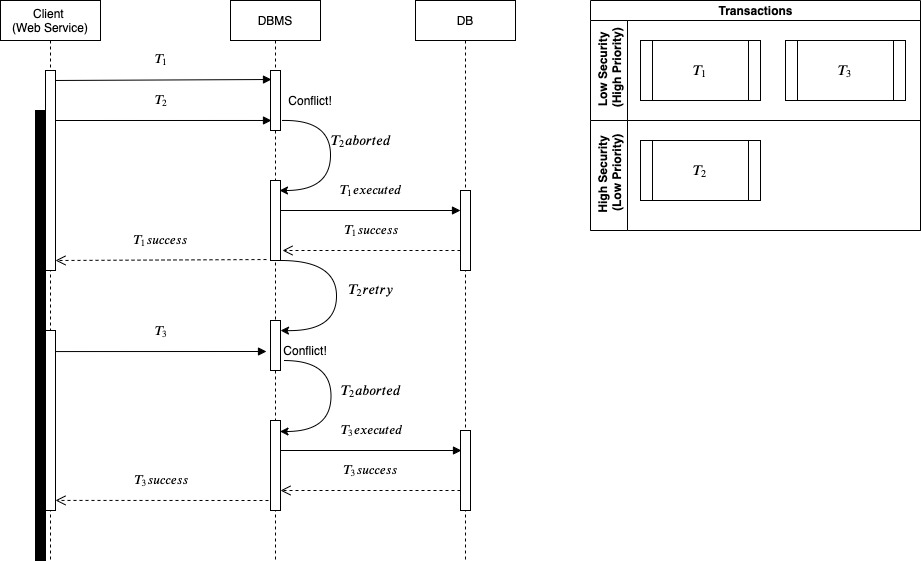
\includegraphics[scale=0.45]{images/TransactionStarvation.jpg}
\caption{Web Service Transaction Starvation}
\label{fig:ws_trans_starvation}
\end{figure}

Figure \ref{fig:ws_trans_starvation} shows an example of three transactions ($T_1$, $T_2$, and $T_3$) entering a system via a web service. $T_1$ and $T_3$ are of a low security classification while $T_2$ is of a high security classification. $T_1$ and $T_2$ enter the system at the same time and are accessing a shared resource between the two transactions. This causes a conflict and in order to prevent a timing covert channel, we abort the higher security transaction, $T_2$. $T_1$ is then able to execute successfully and complete. We then attempt to retry $T_2$ but coincidentally another transaction, $T_3$, is submitted for execution. The same process happens again, $T_2$ is aborted, and $T_3$ is executed successfully. The black vertical bar on the left side of Figured \ref{fig:ws_trans_starvation} shows the process of $T_2$ through all the aborts that happened. This illustrates the starvation of $T_2$ that happens when trying to prevent covert channels.

\subsection{Problem Identified}
\label{mls:poblem_identified}
After analyzing the system structure and architecture of an \ac{MLS} database and seeing a use-case scenario, we see two problems that can be improved upon. The first being the existence of a timing covert channel due to a conflict among low and high security transactions. The second problem identified is the starvation of high security transactions due to the solution that many lock-based concurrency control algorithms present to address timing covert channels. Both of these problems have been addressed in past research (look at \cite{samarati_database_2016} for example) by simply causing transactions of a higher-security classification to abort in order to make way for the lower-security classification and then adding a priority to higher-security transactions in order to prevent starvation.

But the problem with this approach is that there is no flexibility within the solution to abort a problematic low-security transaction. The current solution leverages a binary decision model and priorities within the recovery model to address the side effect of starvation. The real problem is providing a solution that eliminates the timing covert channel with minimal side effects to efficiency and consistency that have to be reconciled. This solution would provide a safe and reliable way to abort both high-security and low-security transactions to prevent covert channels depending on the system environment.

We believe that this problem can be addressed with the dynamic categorization and reputation that the prediction-based scheduler provides in Chapters \ref{chap:prediction_based_scheduler} and \ref{chap:dynamic_reputation}.
\section{Related Work}
\label{mls:related_work}

Multi-level secure databases are a huge area of research due to the security concerns that can arise within these databases and the consequences if a vulnerability is exposed. The consequences have been so great that many users of multiple security classifications use multiple databases with duplicated common resources to prevent any security vulnerability from happening \footnote{This implementation is commonly found in DoD database systems and their Security Technical Implementation Guides (STIGs) \hyperlink{https://public.cyber.mil/stigs/}{https://public.cyber.mil/stigs/}}. However, researchers understand the benefits of having a secure solution contained in a single database system with multiple security levels.

Jajodia et. al. is one of the main motivations for our work (see \cite{jajodia_fair_1998}). In this publication we see a new locking protocol presented specifically for multi-level secure databases that prevents the starvation of lower security classification transactions. In this work, the researchers analyzed the existing two-phase locking protocol with additional policy additions to increase performance. In their analysis they discovered in order to increase performance and prevent starvation by increasing the fairness of all transactions, they needed to restrict the number of low security transactions executing. One quote from the work that motivates our work is,

\begin{displayquote}
"Several concurrency control algorithms that are free from covert channels have been proposed in the literature. Most of these algorithms prevent covert timing channels by ensuring that transactions at lower security levels are never delayed by the actions of a transaction at a higher security level. This can be accomplished by providing a higher priority to low transactions whenever a data conflict occurs between a high transaction and a low transaction."
\end{displayquote}

The prediction-based solution established in Chapter \ref{chap:prediction_based_scheduler} provides a solution to elevate or demote transactions based on transactional attributes that are deemed necessary to properly categorizing a transaction. As a part of the categorization process, the security level in which a transaction resides can be a part of the transaction's attributes necessary for categorization.

Other, more recent, works that have been of influence for this solution involve \cite{mahmoud_encryption_2019} by Mahmoud and Alqumboz, \cite{sun_access_2011} by Ying-Guan Sun, \cite{hedayati_evaluation_2010} by Hedayati et. al., \cite{shanwal_secure_2013} by Shanwal and Kumar, \cite{sapra_development_2014} by Sapra et. al., \cite{kaur_performance_2004} by Kaur, N. et. al., \cite{costich_analysis_1991} by Costich, O.L. et. al., \cite{kaur_feedback_2007} by Kaur, N. et. al, \cite{keefe_database_1993} by Keefe T.F. et. al, and \cite{david_secure_1993} by David N. et. al. All of which have been built up on the work of the Bell–LaPadula Model, Biba Integrity Model, and lattice based security model (LBAC) (work referenced in \cite{bell_secure_1973}, \cite{biba_integrity_1977}, \& \cite{denning_lattice_1976}).
\section{Environment}
\label{mls:environment}

A multi-level secure database is much like any traditional database system. The major difference is the presence of resources, users, and transactions with differing security levels. This can be resources within the system that contain a certain a security level. This can also be true for users who maintain a certain security level and therefore the transactions generated by the user contains a certain security level. Current architecture solutions leverage the Bell-LaPadula model (\cite{bell_secure_1973}) to ensure that current security levels are maintained and data is not accessed inappropriately. The Bell LaPadula Model abides by two main rules to ensure secure data access. The two rules are:

\begin{enumerate}
  \item A subject at a given security level may not read an object at a higher security level. This is known as the Simple Security Property
  \item A subject at a given security level many not write to any object a lower security level. This is known as the * (star) Property
\end{enumerate}

\begin{figure}
\centering
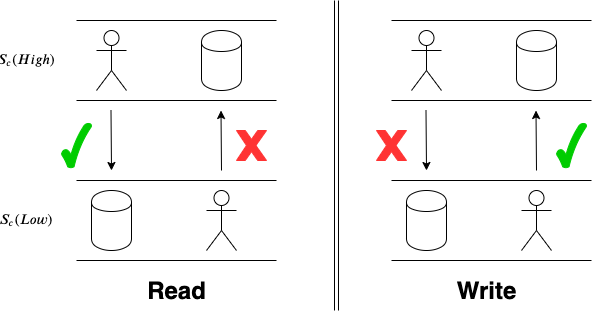
\includegraphics[scale=0.45]{images/BellLapadulaModel.png}
\caption{Bell-LaPadula Model}
\label{fig:bell_lapadula_model}
\end{figure}

Both of these properties are shown in Figure \ref{fig:bell_lapadula_model}. While this ensures proper data access control for security levels, the Bell-LaPadula Model doesn't protect against covert channels that occur due to concurrent transactions. Concurrent transactions cause issues when there are conflicting operations. When there is a conflict, one of the transactions must wait for the other transactions to finish processing before execution can continue processing. The presence (or even absence) of a time delay for the transaction to execute introduces a covert channel. 

A covert channel is a security flaw where a means of communication to transmit unauthorized information is available via the normal means of communication. Timing channels are a form of covert channel where the presence of absence of a execution delay conveys unauthorized information about the underlying system. This work is documented by Girling in \cite{girling_covert_1987}. Timing channels are difficult to prevent and many times requires review of the application source code directly to ensure all operations execute with the same timing delay. Common solutions to prevent covert timing channels in multi-level secure databases when there are conflicting operations is to abort the transaction with a higher security classification. This prevents the transaction with a lower security transaction from detecting a timing delay. The timing delay would communicate to the lower security transaction that resources of a higher security classification were present and therefore leaking unauthorized information. Figure \ref{fig:env_covert_channel_exposure} (referenced from Figure \ref{fig:ws_trans_starvation} in Section \ref{mls:problem_definition}) shows the exposure of a timing covert channel.

\begin{figure}
\centering
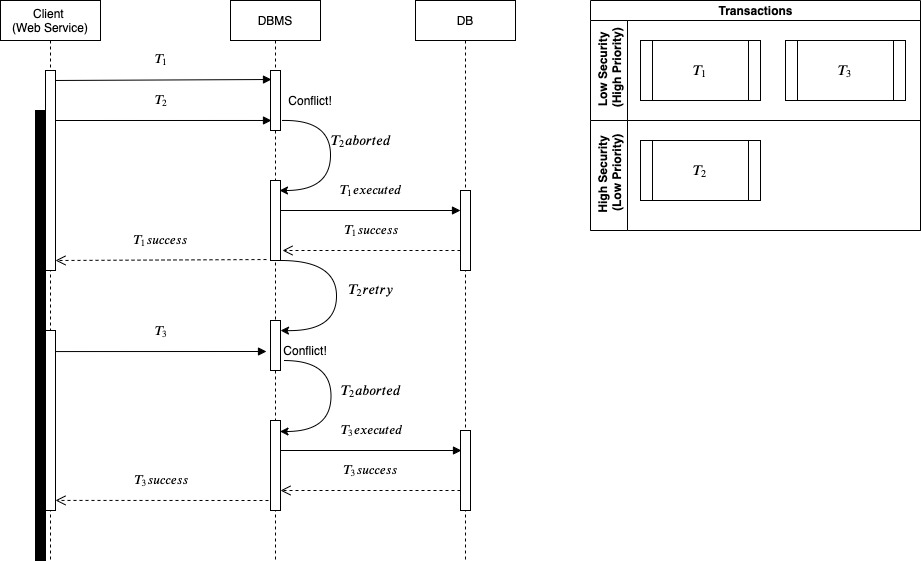
\includegraphics[scale=0.45]{images/TransactionStarvation.jpg}
\caption{Transaction Starvation Exposes Timing Covert Channel}
\label{fig:env_covert_channel_exposure}
\end{figure}
\section{Transaction Quality Measure}
\label{mls:tqm}

In this section we discuss the potential future work for implementing a security classification within the prediction-based scheduler (outlined in Chapters \ref{chap:prediction_based_scheduler} and \ref{chap:dynamic_reputation}) that would address the issues found specifically in \ac{MLS} databases. 

Within the prediction-based solution, there are currently four attributes that allow for a reputation score to be calculated among transactions. Those four attributes are commit ranking, efficiency ranking, user ranking and system ranking (see Definitions \ref{def:commit_ranking}, \ref{def:efficiency_ranking}, \ref{def:user_ranking}, and \ref{def:system_abort_ranking} in Chapter \ref{chap:dynamic_reputation}). This allows for the formation of a reputation score to be calculated for each transaction in the system. Within these reputation scores, there is a dominance structure that causes transactions to be prioritized depending on if dominance can be established (outlined in Definitions \ref{def:strong_dominance} and \ref{def:weak_dominance}). With all of these components in place, we have a foundation for efficient transaction categorization within \ac{MLS} databases.

A potential future state of the system is to use the existing reputation score within the existing prediction-based solution alongside a security label to create a two-tuple Transaction Quality Measure (TQM). This will involve an update dominance structure to ensure the absence of covert channels and also prevent starvation of higher security transactions within the system. The solution would allow for a better decision making model for which transactions are aborted and rescheduled. The new Transaction Quality Measure would take security classification into account, but it would not allow the security classification to be the only dictating factor. Extending the prediction-based solution would allow the other four attributes to be included within the decision process. Figure \ref{fig:existing_reputation_score} is a representation of the existing reputation score defined in Chapter \ref{chap:dynamic_reputation}. Figure \ref{fig:mls_strong_dominance} shows the strong dominance structure of Transaction Quality Measures where $SL$ is the security label and $PV$ is the performance vector representing the existing reputation score. Figure \ref{fig:mls_weak_dominance} shows the weak dominance structure.

\begin{figure}[h]
\captionsetup{justification=centering}
\centering % used for centering Figure

\[\textrm{$RS_{T_{i}}$ = $<w_{i}^{1}\times CR_{T_{i}},w_{i}^{2}\times ER_{T_{i}},w_{i}^{3}\times UR_{i},w_{i}^{4}\times SR_{T_{i}}>$}\]

\caption{Current Reputation Score} % title of the Figure
\label{fig:existing_reputation_score} % label to refer figure in text

\end{figure}

\begin{figure}[h]
\captionsetup{justification=centering}
\centering % used for centering Figure

\[\textrm{
$TQM_{1}(SL_{1},PV_{1}) \geq TQM_{2}(SL_{2},PV_{2})$ iff $SL_{1} \leq SL_{2}$ and $PV_{1} \geq PV_{2}$}\]

\caption{MLS Strong Dominance} % title of the Figure
\label{fig:mls_strong_dominance} % label to refer figure in text

\end{figure}

\begin{figure}[h]
\captionsetup{justification=centering}
\centering % used for centering Figure

\[\textrm{
$TQM_{1}(SL_{1},PV_{1}) \geq TQM_{2}(SL_{2},PV_{2})$ iff $SL_{1} \geq SL_{2}$ and $PV_{1} > PV_{2}$}\]

\caption{MLS Weak Dominance} % title of the Figure
\label{fig:mls_weak_dominance} % label to refer figure in text

\end{figure}

In order to prevent covert timing channels within multi-level secure database, the future solution would leverage the timing delay of the existing prediction-based solution to be used as a "cover story" for the timing difference between transactions of differing security levels. The cover story would allow for transactions to be aborted for conflicting transactions without introducing a covert timing channel for unauthorized disclosure of high security resources.

In summary, there are two well-known problems within multi-level secure databases. The first problem is the existence timing covert channels when transactions of multiple security levels are accessing a common resource. The presence or absence of a time delay provides the indication of high security resources that are available. The second problem, is brought on by the solution to multi-level secure databases. A solution to prevent against covert channels is to abort transactions of a higher security classification so that the time delay does not exist. However, this then causes these transactions to suffer from starvation and will never be executed. The solution presented in this section will address both problems and provide a way forward for more granular decision-making within multi-level secure database systems.

With the prediction-based scheduler in place and a solution for dynamic reputation of transactions, the possibilities for extension within multi-level secure databases is then feasible . Chapter \ref{chap:prediction_based_scheduler} presented the solution and operated under the assumption that the reputation of the transactions were already established. Chapter \ref{chap:dynamic_reputation} focuses on exactly how the transactions establish their reputation and also dynamically increase or decrease their reputation. With this work in place, extending the prediction-based system to multi-level secure databases is now possible.
\section{Additional Future Work}

In this section, we want to outline the future work opportunities of the prediction-based scheduler and how the work can be expanded upon. The work mentioned in this section is not meant to be included in this dissertation, but rather listing outstanding opportunities for the current and proposed work to continue forward.

\subsection{Snapshot Isolation}
Another potential for future work is the ability to perform snapshot isolation within the different categorizations of transactions. This extension will be for both malicious and lower priority transactions that affect the majority of well-performing transactions. In this work we'll use snapshot isolation to execute certain categorizations of transactions on snapshots of the database in order to prevent the effects of low-performing transactions from affecting all transactions. Once the outcome of a transaction has been determined then the snapshot can either be discarded or merged.

\subsection{Prediction-based Scheduling within Linked Databases}
An additional extension is the issue of efficient concurrency control within linked database environments. Currently the Prediction-based solution addresses efficient concurrent transactions within a web-service environment that are contained within a single cluster. This particular area of research will address the problem through the lens of the Prediction-based solution. The difficulty of the problem within this work is adapting the existing framework of correctness built within the Prediction-based solution so that it will scale to linked database systems while preserving its existing capabilities. Figure \ref{fig:system_model_linked_databases} shows the system model for the Prediction-based solution within linked database systems.

\begin{figure}[h]
\captionsetup{justification=centering}
\centering
\includegraphics[width=\textwidth]{images/LinkedDatabase_SystemModel}
\caption{Prediction-based Scheduler within Linked Databases}
\label{fig:system_model_linked_databases}
\end{figure}

\subsection{PostgreSQL \& MySQL}
\label{conclusion:posgressql}
Two very commonly used databases within enterprise applications are \href{https://www.postgresql.org/}{PostgresSQL} and \href{https://www.mysql.com/}{MySQL}. Both of which are open-source relational databases where their code is available to the public for modification and contribution. Open-source applications tend to have very difficult review process which allows for quality code and reliable software. Both of these database management systems have provided their code on Github so that the community can contribute features, bug fixes, and enhancements accordingly. The code for PostgresSQL is located at \href{https://github.com/postgres/postgres}{https://github.com/postgres/postgres} and the code for MySQL is located at \href{https://github.com/mysql/mysql-server}{https://github.com/mysql/mysql-server}.

One opportunity for future work would be to fork one or both of these repositories on a controlled system and implement the algorithms of the prediction-based scheduler within the database management system itself. Currently, the prediction-based scheduler has been proven theoretically in a test environment using an in-memory database. This work has proven the viability of the solution and the consistency that it provides. By placing the prediction-based solution in the database management system itself, it would provide a beautiful marriage of academia and industry coming together for a common solution. The initial goal would be to get the algorithms working on a mirrored fork initially in a controlled test environment, then moving that solution to a clustered environment to ensure scalability, and eventually providing an official pull request of the prediction-based scheduler to the code maintainers of both systems so the solution would then be available to the general public in future releases. This future work provides a direct road map from academic theory to impacting the global industry for the benefit of the masses.
\section{Conclusion}
\label{mls:conclusion}
In summary, there are a multitude of opportunities to extend the current work into new realms. The prediction-based scheduler along with dynamic transaction reputation provides a system of consistency and scalability that can be extended into multi-level secure databases, linked databases, and other systems of databases. This contribution will provide a foundation for future researchers to extend into realms of database scheduling and transaction execution that have not been discussed before.
 %% Chapter 5

\chapter{Conclusion}
\label{chap:conclusion}

\section{Concluding Remarks}
\label{conclusion:concluding_remarks}
In this proposal, we have first analyzed the shortcomings to existing web service database transactions. These shortcomings involve the need for compensation transactions that, ultimately, are unnecessary overhead if A.C.I.D transaction properties can be leveraged. We analyzed the current solutions involving compensation transactions and maintaining consistency within a web service environment. As a result of this analysis, research and prototyping led to the development of a prediction-based solution. The final solution dynamically uses different concurrency control mechanisms depending on the attributes of the transaction. In the current work we have formally proven that this solution will ensure consistency by using dynamic concurrency control mechanisms (published in \cite{ravan_ensuring_2020}).

Second, we have proposed the needed extensions to the work that will address three additional areas of improvement. The first area is expanding the prediction-based solution to a multi-level secure database environment where multiple security classifications exist. This involves extending the existing two-dimensional categorization graph to a three-dimensional graph for all transactional attributes to prevent the existence of covert timing channels that can appear due to differing security classifications. By doing so we provide a cover story for the transactional environment that enables the promotion of high security transactions without the disclosure of a covert timing channel.

The final effort will be the final extension leveraging all phases of the dissertation. This effort will focus on the formal categorization of transactions before entering the prediction-based solution. In this effort we extract the extrinsic attributes from the intrinsic attributes to reveal transactional classes that can be identified and grouped. From there, those classes contain a reputation that is managed dynamically in order to grow with the environment. That then allows the categorization of transactions to be promoted and demoted based on the reputation.

% The final effort will be the final extension leveraging all solutions. This effort will use Snapshot Isolation for low-performing and malicious transactions. With the current and proposed research the overall contribution will ensure consistency among web service transactions. The contribution will also minimize the effects of malicious and poorly performing transactions within a web service environment.
% \section{Future Work}
\label{conclusion:future_work}
In this section, we want to outline the future work opportunities of the prediction-based scheduler and how the work can be expanded upon. The work mentioned in this section is not meant to be included in this dissertation, but rather listing outstanding opportunities for the current and proposed work to continue forward.

\subsection{PostgreSQL \& MySQL}
\label{conclusion:posgressql}
Two very commonly used databases within enterprise applications are \href{https://www.postgresql.org/}{PostgresSQL} and \href{https://www.mysql.com/}{MySQL}. Both of which are open-source relational databases where their code is available to the public for modification and contribution. Open-source applications tend to have very difficult review process which allows for quality code and reliable software. Both of these database management systems have provided their code on Github so that the community can contribute features, bug fixes, and enhancements accordingly. The code for PostgresSQL is located at \href{https://github.com/postgres/postgres}{https://github.com/postgres/postgres} and the code for MySQL is located at \href{https://github.com/mysql/mysql-server}{https://github.com/mysql/mysql-server}.

One opportunity for future work would be to fork one or both of these repositories on a controlled system and implement the algorithms of the prediction-based scheduler within the database management system itself. Currently, the prediction-based scheduler has been proven theoretically in a test environment using an in-memory database. This work has proven the viability of the solution and the consistency that it provides. By placing the prediction-based solution in the database management system itself, it would provide a beautiful marriage of academia and industry coming together for a common solution. The initial goal would be to get the algorithms working on a mirrored fork initially in a controlled test environment, then moving that solution to a clustered environment to ensure scalability, and eventually providing an official pull request of the prediction-based scheduler to the code maintainers of both systems so the solution would then be available to the general public in future releases. This future work provides a direct road map from academic theory to impacting the global industry for the benefit of the masses.     %% Honors theses are required to 
                          %% have an unnumbered chapter
                          %% for conclusions.  The file
                          %% Conclusion.tex should begin
                          %%   
                          %% \chapter*{Conclusion}
                          %% followed by the appropriate
                          %% text.

\printbibliography %%  This is the command to use to
			       %%  insert the bibliography if you are using
                           %% the biblatex.sty package.  See the 
                           %% uscthesisdoc.pdf documentation for
                           %% for alternative bibliographic systems.     

\Appendix                 %% Use this command if you have one 
                          %% appendix. Use \Appendices if you 
                          %% have more than one.
	
\chapter{DRP Results}
\label{chap:appendix_drp_results}

This section of the appendix presents more of the experimentation results from the dynamic reputation prototype. Here we discuss the background of the formulation of the use cases used in Chapter \ref{chap:dynamic_reputation}.

% \input{chapters/7__Appendix/sections/drp_results}
 %% Calls toolong.tex which contains
                          %% an appendix. After issuing the 
                        %% command \Appendix or \Appendices
                        %% you must use \input not \include
                        %% to load the first appendix.
                        
\end{document}
%%%%%%%%%%%%%%%%%%%%%%%%%%%%%%%%%%%%%%%%%%%%%%%%%%%%%%%%%%%%%%%
